%----------------------------------------------------------------------
%	PART 3 : Cyberdefense
%----------------------------------------------------------------------

%==========================
\chapter{Introduction à la SECOPS}
\ulindex{SECOPS}

%-------------------------------------------------------------
%               FR CYBERDEF SECOPS COURSE
%                           SECOPS
%.                    Vulnerability/Threat/Incident
%
%                   Introduction Cyberdefense
%                    chap-Cyberdef-intro.tex
%
%                     2020 eduf@ction
%-------------------------------------------------------------
\uchap{Chapitre introductif de la Partie 3 du cours SEC 101 - CYBERDEF}

% ***** CHAPTER CYBERDEF


\section{SECOPS et cyberdéfense}

Mettre en place des stratégies de cyberdéfense \ulindex{Stratégie de cyberdéfense}, c'est partir du principe que l'entreprise sera attaquée et que l'enjeu des équipes est de se préparer à des attaques pouvant violemment impacter l'entreprise. Pour cela, l'entreprise doit anticiper, détecter à temps et réagir vite pour réduire l'impact.

	\subsection{Des opérations de cyberdéfense d'entreprise}
	
C'est dans ce contexte de sécurité  que doit s'organiser cette cyberdéfense opérationnelle et se structurer autour des axes qui caractérisent une posture de cyberdéfense d'entreprise : 
	
\begin{itemize}
  \item Le renseignement : 
  				\begin{itemize}
  					\item sur les menaces  : les attaquant et leurs intentions, leurs techniques et outils, les sources compromises,
  					\item sur les vulnérabilités : des logiciels, et des structures organisationnelles,
			\end{itemize}
  \item La détection d'attaques ou de menaces dormantes ou cachées;
  \item La mise en alerte, ou la réponse à incidents pour aller à la gestion de crise;
  \item La neutralisation de sources malveillantes.
\end{itemize}
	
\subsection{Veille et renseignement}

Au coeur des opérations de cyberdéfense, le renseignement reste le moteur de l'anticipation.  Une grande partie des attaques exploitent des failles ou des vulnérabilités. Être au plus tôt au courant de l'existence d'une vulnérabilité sur un système utilisé par l'entreprise est le premier stade d'une veille pour ANTICIPER une attaque potentielle basée sur cette faille.

Toutes les attaques ne sont pas liées à l'utilisation d'une faille technique, il existe d'autres marquants ou indicateurs qui peuvent être surveillés pour évaluer les risques. Nous verrons dans le chapitre sur la détection, que les marquants des menaces sont souvent des données techniques qui peuvent caractériser l'attaque. l'attaquant, les techniques utilisées...
Par ailleurs le renseignement permet aussi de détecter des fuites de données, ou des informations sensibles compromises en surveillant les sites spécialisés.
On peut citer le célèbre \textbf{\ulink{https://haveibeenpwned.com}{';--have i been pwned?}} qui indique si une adresse électronique utilisée comme identifiant de compte a été compromise lors d'un vol de données sur un site. 

L'ensemble des informations liées aux menaces s'appelle de la \UKword{Threat Intelligence ou Cyber-Threat Intelligence (CTI)}, et celles liées aux vulnérabilités  classées dans la dynamique \UKword{Vulnerability Intelligence}.

\upicture{Latex/Sources/EDU/Pictures/img-intelligence}{Les axes du renseignement cyber}{0.5}{lblintelligence}

\subsection{VTI(Vulnerabilty/Threat/Incident)}

\upicture{Latex/Sources/EDU/Pictures/img-VTIsimple}{Les axes du renseignement cyber}{0.7}{lblVTIsimple}

Le triptyque VTI (Vulnérabilités/Failles, Menaces/Attaques, Incidents/Alertes), est souvent présenté comme le coeur des activités de sécurité opérationnelle. 


La sécurité opérationnelle c’est l’ensemble des processus opérationnels qu’il faut mettre en place et évaluer au quotidien afin de réduire la surface d’exposition du système d’information aux risques, mais aussi réduire l'impact en cas d'attaque. 

On y trouve en particulier : 

\begin{itemize}
  \item Les audits techniques, pentests, scan : pour identifier les fragilités, mais aussi la cartographier les actifs, les acteurs ...,
  \item Les systèmes de détection comme le SIEM, de chasse comme le Threat Hunting ...,
  \item Les mécanismes de remédiation, les techniques et outils de forensique.
\end{itemize}

Toutes ces actions génèrent au sein de l'entreprise de l'information, souvent à destination d'acteurs différents mais participant globalement à l'objectif de cyberdéfense.

\subsection{Fusion Center}

Les préoccupations des responsables de cette sécurité opérationnelle restent encore l'accès et le partage de l'information car dans le cycle de gestion du risque et de réduction de la surface d'attaque. Le terme \UKword{Fusion Center} est historiquement lié aux attentats du 11 septembre 2001, qui avaient montré les lacunes de partage de l'information entre les services de police et renseignements américains face à cette attaque. Repris par les experts de la cybersécurité, pour gérer les menaces. 
La sécurité opérationnelle est gérée généralement par deux principales structures : le SOC, en charge de la détection, de la qualification et de la gestion des incidents ; et le CSIRT, responsable de la gestion de crise, de l’investigation numérique, de la veille et de la Threat Intelligence.


\upicture{Latex/Sources/EDU/Pictures/img-fusioncenter}{Fusion Center et CSOC}{0.7}{lblfusioncenter}

\begin{itemize}
  \item Automatiser la \textbf{création de règles} basées sur des menaces avérées  et détecter de manière avancée avec le \UKword{Machine Learning}
  \item Automatiser le \textbf{processus de management }des incidents avec en  particulier les SOAR (Security Orchestration, Automation et Response) outils d’aide et d’automatisation de la réaction aux incidents de sécurité.
  \item Adapter \textbf{l’organisation} à cette automatisation
  \item et surtout automatiser la \textbf{collecte et la distribution} de l'information dans les différents services grâce à un \g{Centre de Fusion de l'information et du renseignement}.
\end{itemize}


\subsection{Entrainement à la cyberdéfense}

En matière de cybersécurité, les organisations sont confrontées à la persistance des cyberattaques, combinées à la montée en puissance de nouvelles menaces et ne sont pas suffisamment préparées à anticiper les incidents et à y apporter les réponses adéquates. De nombreuses études continuent à montrer  que la formation du personnel demeure le défi premier, se traduisant par un investissement conséquent de la part des organisations.

L’entraînement répond à différents objectifs de l'entreprise  :
\begin{itemize}
  \item Sensibilisation des acteurs (salariés, décideurs, managers) aux risques « cyber ». Ces entrainements, relativement brefs et regroupant qu'une partie des acteurs  permettent d’illustrer concrètement les menaces. Il permet en particulier de l'illustrer concrètement les impacts des cyberattaques sur une entreprise notamment pour les niveaux stratégiques;
  \item   Evaluation du dispositif de sécurité et de gestion de crise en particulier pour les évaluations autour des travaux de PCA/PRA avec l'ISO 22301. L’objectif est d'évaluer toute la chaîne opérationnelle, des équipes techniques informatiques et sécurité, au top management sur l'ensemble de structures de la résilience;
  \item Entraînement des équipes techniques, par exemple au sein des SOC (Security Operation Center). Cela suppose de s’appuyer sur des environnements de simulation informatique représentatif de la réalité pour s'adapter à l'évolution des attaques (Outils de Range en particulier);
\end{itemize}


Pour répondre à ces besoins, trois niveaux d’entraînement doivent donc être distingués :

\begin{itemize}
  \item Des entraînements techniques au niveau des opérations. Ces entraînement peuvent intervenir dans le cadre de formations des équipes;
  \item Des entraînements managériaux ou niveau des managers de proximité ou des COMEX. La durée de ces entraînements dépend des objectifs de montée en compétence. Pour une  sensibilisation de COMEX,  la durée doit être adaptée et courte (de l'ordre d'une demi journée). Les entraînements  ou exercices peuvent doivent être réguliers, une fréquence d'exercice annuelle est recommandée.
  \item Des entraînements mixtes associant des populations techniques et non techniques, afin de traiter l'inter-dépendance des différentes structures engagées.
\end{itemize}



\subsection{Gestion de crise}

Les opérations de sécurité opérationnelle doivent embarquer le processus de gestion de crise de l'entreprise, on trouvera dans le chapitre de gestion des incidents la manière donc les opérations de cybersécurité peuvent s'intégrer à des processus de gestion de crise existants ou comment créer des processus spécifiques à la cyber-crise. En effet, une des particularités des cyber-crises c'est que le systèmes d'information et de communication peut lui aussi être compromis, et que la confiance dans les systèmes informatiques de gestion peut être altérée, ou ces systèmes totalement inopérants.  

\section{Range et Simulation}

Les cyber-ranges, environnements de simulation informatique, dédiés non seulement à l’expérimentation des technologies, mais également à la formation par la pratique et à l’entraînement du personnel, constituent une réponse à l'enjeu de vision globale.  Initialement développés dans un cadre militaire,  les  cyber-ranges intéressent aujourd'hui l’ensemble de l’écosystème de cybersécurité. Ils offrent des conditions d’entraînement proches du réel, tant dans les topologies réseau reconstituées que dans les technologies de sécurité déployées. Ils fournissent un environnement d’affrontement informatique permettant une nouvelle approche de la formation axée sur l’opérationnel.

Il existe de nombreux outils d'entraînements. La majorité sont construits sur des technologies de virtualisation.
L’environnement de simulation technique est donc basé sur un « bac à sable » numérique (une sorte de paillasse numérique) offrant notamment des capacités de :
\begin{itemize}
  \item Virtualisation de postes de travail et de serveurs  et de tous autres composants informatique ou réseaux. l'environnement de simulation informatique peut être  « hybride » lorsqu’il permet également de connecter des équipements physiques (routeur, sonde, automate industriel...) ou des appliances ;
  \item Virtualisation des différentes couches de transports, de stockage et de traitement ( couche réseau pour les liens et les équipements, couches base de données et infrastructures de base : Annuaire, Infrastructure de gestion de clefs, ...) ; 
  \item  Création de scénarios pédagogiques ou de situations tactiques pour fournir des contextes d'entraînement et de formation ;
  \item  Simulation et Génération de trafic pour donner de la vie au système.

\end{itemize}

L'entraînement est une solution pour dynamiser les activités de cyberdéfense.


\toolsbox{CyberRange-Airbus}{range}
\toolsbox{Hynesim}{range}
\toolsbox{EDUYesWeHack}{range}


\upicture{Latex/Sources/EDU/Pictures/img-range}{Entrainement}{0.8}{lblrange}

Sur le plan humain,  l'utilisation d'un cyber-range se construit autour de deux équipes que nous explorerons dans les chapitres sur la gestion des vulnérabilités et la gestion des menaces :

\begin{itemize}
  \item La « Red-Team », composée de hackers éthiques professionnels (les PENTESTEURS). Ceux-ci reproduisent des attaques ciblées et d’ampleur et de complexité croissante, de nature à challenger la défense tout au long de l’entraînement ;
  \item  La « Blue-Team », chargée de la défense des réseaux et systèmes d’information (le SOC),, qui est donc constituée des apprenants participant au programme d’entraînement ou de formation.
  \item On découvre maintenant dans les entreprises des « Purple-Team » assurant une activité mixte de lutte contre la malveillance couplée à de la chasse "aux failles" et "aux menaces". 
\end{itemize}


%Vous pouvez trouver une document intéressant sur \ulink{https://www.defense.gouv.fr/content/download/502443/8528007/file/OBS_Monde cybernétique_201703.pdf}{le site du ministère des armées} 

% https://www.cloudrangecyber.com/ (autre Range)




%-------------------------------------------------------------
%               FR CYBERDEF SECOPS COURSE
%                                        SECOPS
%.                    Vulnerability/Threat/Incident
%
%                                    Introduction
%                                chap-VTI-intro.tex
%
%                              2020 eduf@ction
%-------------------------------------------------------------
\uchap{Chapitre introductif de la Partie 3 du cours SEC 101 (VTI-INTRO)}


%=======================================
\section{Sécurité opérationnelle}
%--------------------------------------------------------------

En terme de gouvernance, après avoir construit une structure de sécurité cohérente sur les aspects de gestion des flux, de gestion des accès et des identités, et construit une gouvernance efficace sur la base de l'\uindex{ISO27001}, il est  nécessaire de maintenir le niveau de sécurité de l'entreprise ou du système. La dynamique de sécurité de l'entreprise en exploitation nécessite une organisation et des politiques orientées vers cette efficience de l'anticipation, de la détection et de la réaction que nous avons présentées comme le volet cyberdéfense de la cybersécurité de l'entreprise.


% begin frame 
\mode<all>{\texframe{sécurité opérationnelle}{Dans le cycle de vie}
{
Dans certains ouvrages ce processus est dénommé  \g{Maintien en Condition de sécurité}. En utilisant  les termes anglo-saxons définissant le cycle des projets, nous pourrions positionner ses activités dans la phase dite de  \textbf{RUN}. Les autres phases en amont pouvant être définies comme : 

\begin{itemize}
 \item \textbf{THINK/DESIGN} : Des risques évalués à la politique sécurité établie en fonction des risques ;
 \item \textbf{BUILD}: De la politique de sécurité déployée à la construction d’une sécurité implémentée;
\end{itemize}
}} % end frame




% begin PRZ==========================
\begin{frame}
\frametitle<presentation>{sécurité opérationnelle}
\framesubtitle<presentation>{l'activité RUN}
% end header PRZ======================
\upicture{Latex/Sources/EDU/Pictures/img-thinkrun}{les phases du cycle de vie}{0.7}{lblthinkrun}

Et nous classons donc dans la dernière phase du cycle de vie : les activités d'exploitation de la sécurité, \textbf{RUN} : Des évènements de sécurité gérés à une \textbf{Cybercrise} maitrisée, ce que certains appellent \textbf{\uindex{SECOPS}} : \g{\uindex{sécurité Opérationnelle}}.
\end{frame}
% end PRZ ===========================


% begin PRZ==========================
\begin{frame}
\frametitle<presentation>{Objectifs adaptés aux finalités}
\framesubtitle<presentation>{de l'activité de l'entreprise}
% end header PRZ======================
Ce modèle se développe bien entendu en fonction des finalités de l'entreprise.

\begin{itemize}
    \item Soit nous sommes dans \textbf{une dynamique entreprise} et ces processus sont ceux mis en place pour s'assurer que  l'ensemble de actions sont prises en compte pour maîtriser les fragilités dont les vulnérabilités informatiques, détecter les menaces tant en anticipation que pendant des attaques (bruyantes, ou discrètes), et réagir pour maintenir l'activité et limiter l'impact.
    \item  Soit nous sommes \textbf{fabricant d'un produit ou d'un service}, et au delà des engagements sécuritaires de toute entreprise (cf. ci-dessus) des processus de \g{maintien en condition de sécurité} des produits et services sont à ajouter pour maîtriser les vulnérabilités, les correctifs et leur cycle de vie  (audit, communication, gestion des découvertes de fragilités par des tiers, rémunération de BugHunters ...).
\end{itemize}
\end{frame}
% end PRZ ===========================

% begin PRZ==========================
\begin{frame}
\frametitle<presentation>{sécurité opérationnelle}
\framesubtitle<presentation>{Une définition}
% end header PRZ======================
 Le terme de \g{sécurité opérationnelle}, est relativement jeune dans l’histoire de la sécurité des technologies de l’information. Le terme de \uindex{SSI}(sécurité des Systèmes d’Information) était né pour distinguer des disciplines qui s’attachaient à protéger l’information qui circulent dans les systèmes d'information de l’entreprise (cf. protection et classification de l’information) vis à vis de la sécurité des biens et des personnes. La sécurité des réseaux et la sécurité informatique ont été les précurseurs de la cybersécurité, le cyber recouvrant en un seul terme, les enjeux de sécurité liés au réseau et à l’informatique, mais plus largement à la sécurité de l'économie numérique.
\end{frame}
% end PRZ ===========================

Comme nous l’avons abordé dans l'introduction et dans les chapitres précédents, la cybersécurité est un domaine vaste qui regroupe de nombreuses disciplines. Elle peuvent intervenir dans des cycles projets pour construire des systèmes sûrs ou pour assurer la continuité d’activité et la protection des patrimoines dans l'entreprise. Il faut aussi, penser à y ajouter aussi tout un espace de gestion des conformités (législatives, réglementaires, normatives, contractuelles).


C’est plutôt dans un contexte d'opération sécurité au quotidien que l’on parle de sécurité opérationnelle. Ces activités opérationnelles supportent donc le maintien en condition de sécurité au quotidien de l’entreprise. En France, au sein des armées, on parle de lutte informatique défensive permettant de différencier les activités des Cyber-défense des activités de Cyber-protection. Ces activités sont à opposer à la lutte informatique\g {offensive} qui ne sera pas abordé dans c\ecours car elle relève de prérogative des états et non des entreprises. Nous aurons toutefois l'occasion d'aborder le \textbf{Hackback}, dans un prochain.
La sécurité opérationnelle ajoute par ailleurs à son périmètre de surveillance de l'intérieur de la zone de responsabilité de l'entreprise SI, réseaux sociaux, services cloud ...), celle extérieure à l'entreprise via des mécanismes de veille sur la menace et de surveillance des compromissions potentielles. Nous pourrions évoqué l'image d'une cité où \g{Les murs sont épais et solides, les douaniers sont aux portes de la cité, la police doit toutefois veiller à la sécurité des biens et des citoyens dans la ville, car certains sont néanmoins des brigands. Quand à l'armée, elle veille aux frontières du pays informée par des agents à l'étranger}.

On traitera donc cette partie avec une équivalence dans les terminologies suivantes :

% begin PRZ==========================
\begin{frame}
\frametitle<presentation>{Plusieurs terminologies, une dynamique}
% end header PRZ======================
	\begin{itemize}
		\item Maintien en condition de sécurité (\uindex{MCS}); 
		\item Sécurité opérationnelle (\uindex{SECOPS});
		\item Lutte informatique défensive (\uindex{LID});
		\item Cyberdéfense au sens de la cyberdéfense d'entreprise (CYBERDEFENSE).
	\end{itemize}
\end{frame}
% end PRZ ===========================

Le but de cette sécurité opérationnelle est d’être au coeur de l’action de la sécurité de l’entreprise. En effet, la sécurité de l’entreprise est une propriété multiforme. Elle est d’abord statique dans la mesure où elle correspond à un niveau de confiance dans l’environnement pour conserver la disponibilité, la confidentialité et l’intégrité de l’entreprise. Cette forme statique est souvent liée à la conformité de l’entreprise, aux différents référentiels sécuritaires (ISO27000, GDPR, LPM, NIS ...), mais surtout aux objectifs sécurité de l'entreprise face à ses risques et aux exigences de sécurité des clients souvent inscrites dans des plans d’assurance sécurité (Cf. PAS). 
Elle est aussi dynamique car c’est aussi une propriété systémique qui mesure la capacité à anticiper les menaces, identifier les fragilités , détecter en temps réel les attaques et réagir à temps ou au pire disposer des capacités de revenir dans un état de fonctionnement compatible avec la survie de l’entreprise (Modes dégradés par exemple).
Le système évolue, faisant apparaitre ici et là de nouvelles fragilités, l’entreprise se transforme, vit, suscitant de nouveaux potentiels d’attaques. L’entreprise doit s’organiser pour disposer de fonctions opérationnelles adaptées et dédiées à cette activité. Ces fonctions nécessitent des savoirs, des savoirs-faire et de l’outillage. C’est l’ensemble de ces techniques que nous allons tenter d’aborder dans c\edoc.

Globalement, on peut remarquer que le cycle de vie est à prendre dans le sens inverse de notre présentation. Dans les entreprises moins matures en gouvernance de la sécurité, la dynamique de cette sécurité opérationnelle est la première visible et opérée. L'entreprise va réagir le plus souvent dans une dynamique de réponse immédiates aux problèmes de sécurité sans pour autant investiguer plus avant dans les fragilités globales. Les mécanismes de cybersécurité sont donc construits dans une entreprise peu mature dans le sens suivant :

% begin PRZ==========================
\begin{frame}
\frametitle<presentation>{Enjeux SECOPS}
% end header PRZ======================
	\begin{itemize}
		\item Répondre aux incidents de sécurité, tenter de répondre à la question : \g{qui nous attaque et pourquoi}; 
		\item Améliorer les filtrages;
		\item Couvrir les vulnérabilités découvertes;
		\item Rechercher les vulnérabilités existantes dans le périmètre de responsabilité ;
		\item Anticiper les attaques;
		\item Anticiper les risques informatiques;
		\item Anticiper les risques sur l'information;
		\item Anticiper la menace.
	\end{itemize}
\end{frame}
% end PRZ ===========================

\section{Lutte contre la menace}

La finalité de cette défense d’entreprise est de lutter contre ces attaques qui ne sont pas qu’informatiques. L’attaquant peut utiliser des scenarii utilisant de nombreux vecteurs qui peuvent utiliser des fragilités organisationnelles ou humaines. On peut dire qu’une attaque est une fonction complexe, qui peut viser ou utiliser de nombreux facteurs internes et externes à l’entreprise. Ces facteurs constituent ce que certains nomment l’environnement numérique ou digital de l’entreprise. Cet environnement est globalement constitué de l’ensemble des outils, services, moyens informatiques ou réseaux utilisés par l’entreprise.
Mai 2017 a été un tournant dans la prise de conscience de la menace de la part des entreprises. Le Rançon-logiciel WannaCry a plus fait trembler les médias que les entreprises, mais a permis de faire comprendre au grand public les enjeux des menaces informatiques.


\begin{nota}[Paramètres d’une attaque]
\begin{equation}
Attaque = Fonction \left[ Fragilit\acute{e}s\,HOT\, Entreprise\otimes Gains\,Escompt\acute{e}s\,PF \right]
\end{equation}
\end{nota}

\begin{itemize}
	\item Fragilités HOT : Humaines, Organisationnelles, Techniques 
	\item Gains pour l'attaquant : Idéologiques, Politiques, Financiers, ...
\end{itemize}

On peut classer la majorité des attaques informatiques dans quatre grandes classes :

% begin PRZ==========================
\begin{frame}
\frametitle<presentation>{Grandes typologies des attaques numériques}
% end header PRZ======================
\begin{itemize}
\item Attaques \textbf{d’interception} d’information, vols par écoutes passives ou actives dans les flux transitant entre un émetteur et un récepteur;
\item Attaques par \textbf{déni de services}, généralement sur le réseau : Ce type d’attaque est une atteinte à la DISPONIBILITE du système, basé souvent sur la saturation d’une capacité de traitement. Le système saturé dans l’exécution de certaines de ses fonctions, ne peut plus répondre aux demandes légitimes, car il est occupé à traiter d’autres sollicitations;
\item Attaques par \textbf{exploitation de failles }logiciels : Ce type d’attaque va utiliser une vulnérabilité, d’un système d’exploitation ou d’un logiciel pour exécuter du code malveillant. Ce code réalisera alors sa mission;
\item Attaques par \textbf{exploitation de défauts} de configuration : Ce type d’attaque utilise simplement un ou des défauts de configuration pour que légitimement l’agresseur puisse dérouler un scénario, qui pourra lui donner par exemple des droits particuliers pour conduire des attaques.
\end{itemize}
\end{frame}
% end PRZ==========================

Nous pourrions remarquer que ce nombre est relativement faible. Toutefois, la vrai difficulté réside dans la multiplicité des vulnérabilités, et des défauts de configuration. Les développeurs réalisent des logiciels possédant des failles (vulnérabilités), les utilisateurs ou les administrateurs déploient des systèmes en faisant des erreurs de configuration, ou ne les configurent que très rarement en pensant à la malveillance.

Les motivations des attaquants sont nombreuses, et leurs objectifs variés :

% begin PRZ==========================
\begin{frame}
\frametitle<presentation>{Motivations de l'attaquant}
% end header PRZ======================

\begin{itemize}
\item obtenir un accès au système pour s’y maintenir en attendant une opportunité ;
\item récupérer de l’information, secrets, données personnelles exploitables (en gros toute information ayant de la valeur)
\item récupérer des données bancaires ;
\item s'informer sur l'organisation (entreprise de l'utilisateur, etc.) ;
\item troubler, couper, bloquer le fonctionnement d'un service (les \uindex{rançongiciels} entre dans cette catégories) ;
\item utiliser le système d’un utilisateur, pour rebondir vers un autre système ;
\item détourner les ressources du système d’un utilisateur (utiliser de la bande passante, utiliser de la capacité de calcul) ;
\end{itemize}
\end{frame}
% end PRZ==========================

Bien entendu, il n’y a que très rarement un seul objectif, c’est la combinaison des méthodes d’attaques, des objectifs unitaires qui définissent globalement une mission ou un objectif final. L’exploitation de vulnérabilités au sein de l’entreprise va permettre le déploiement par l’attaquant d’un scénario.

\subsection{Politiques et Stratégies}

% begin PRZ==========================
\begin{frame}
\frametitle<presentation>{Politique vs stratégie}
% end header PRZ======================

\upicture{Latex/Sources/EDU/Pictures/img-cyclevie-pol-strat}{Positionnement de la sécurité opérationnelle}{0.9}{lblpol-strat}

\end{frame}
% end PRZ==========================

A partir des risques identifiés, l’entreprise a posé des politiques de sécurité qui ont permis de mettre en place des mesures de sécurité. Ces mesures sont d’ordre techniques avec des systèmes de sécurité, ou des SI avec des architectures particulières, mais aussi d’ordre organisationnel avec des procédures et des mécanismes à respecter.
L’ensemble de cette dynamique construit un niveau de sécurité qu’il va être nécessaire de maintenir dans le temps. Toutefois ce niveau de sécurité n’est pas suffisant pour une simple et bonne raison : la menace évolue, les vulnérabilités apparaissent (découvertes, ou créées), la valeur\g{marchande} des actifs d’une entreprise change aussi. 
Les occurrences de ces éléments de vie sont considérés comme des évènements qu’il convient de détecter avec suffisamment d’avance sur l’attaquant pour pouvoir le plus rapidement les prendre en compte.

La gestion des événements qui peuvent être une source de mesure de l’évolution du niveau de sécurité de l’entreprise est au coeur des stratégies de cyberdéfense. Ces évènements sont corrélés avec des sources provenant de deux processus particuliers qui seront décrits dans ce c\edoc.

% begin PRZ==========================
\begin{frame}
\frametitle<presentation>{Politique vs stratégie}
% end header PRZ======================
Il est à noter qu'un attaquant ne raisonne pas en politiques d'attaque face à une politique de sécurité, mais par des stratégies auxquelles il faut opposer aussi par des stratégies de défense, dont 

\begin{itemize}
\item Recherche des vulnérabilités : Processus qui permet de rechercher, découvrir, couvrir les vulnérabilités ou fragilités de l’entreprise ou ayant un impact sur l’entreprise que celles-ci soient techniques, humaines ou organisationnelles ;
\item Prévention de la menace : Processus qui permet de connaître les menaces directes sur l’entreprise ou potentielles afin d’anticiper et/ou se préparer à un type d’attaque.
\end{itemize}
\end{frame}
% end PRZ==========================

C’est la confrontation entre les vulnérabilités, les menaces et la détection de l’activité de l’entreprise qui va permettre d’être efficace dans le processus de réponse. Il y a de nombreuses manière d’aborder la cyberdéfense d’entreprise.

C\edoc présente donc une dynamique de cyberdéfense en trois\g{volets }

% begin PRZ==========================
\begin{frame}
\frametitle<presentation>{3 volets d'une cyberdéfense}
% end header PRZ======================


\begin{itemize}
\item Gestion des vulnérabilités (\textit{Vulnerability Management and CERT}) : maîtriser ses vulnérabilités mais aussi surveiller l’environnement technologique. 
\item Surveillance, Détection de la menace (\textit{Event and Threat Management}) : Analyser en temps réel l’environnement protégé mais aussi surveiller l’écosystème lié à la menace pour anticiper 
\item Gestion des incidents et réponse aux incidents (\textit{Incident Response – CSIRT}) : Réagir en cas d’incident et assurer la remédiation
\end{itemize}

\end{frame}
% end PRZ==========================


% begin PRZ==========================
\begin{frame}
\frametitle<presentation>{3 volets d'une cyberdéfense}
% end header PRZ======================
\upicture{Latex/Sources/EDU/Pictures/img-triangle}{Des 3 des volets de la sécurité opérationnelle}{0.6}{lbltriptyque}

\end{frame}
% end PRZ==========================

Ces trois volets ne sont pas les seuls qui concourent à la cyberdéfense d’entreprise, mais il en reste les trois faces principales. Il est à noter que ces trois volets correspondent aussi en France à trois référentiels de qualification de l’ANSSI des prestataires de services de cybersécurité au profit des entreprises. Ces labels sont obtenus par les entreprises qui respectent un cahier des charges rigoureux sur le plan de l'éthique, du professionnalisme, et de la compétence des experts intervenants. Il y trois cadres principaux de certifications sont :

% begin PRZ==========================
\begin{frame}
\frametitle<presentation>{Référentiels ANSSI}
% end header PRZ======================
\begin{itemize}
\item PASSI : Prestataire d’Audit de la sécurité des systèmes d’information ;
\item PDIS : Prestataire de détection d’incident de sécurité ;
\item PRIS : Prestataire de réponse à incident.
\end{itemize}

Ces trois référentiels définissent l’ensemble des exigences d’assurance pour\g {qualifier} des prestataires de services en cybersécurité sur ces trois thématiques. En effet, il serait en effet important de confier la recherche de ses vulnérabilités, leurs remédiations à des sociétés de confiance. 
\end{frame}
% end PRZ==========================
A ces trois volets il ne faut pas oublier, le volet administration des briques informatiques et de télécommunications de l’environnement de l’entreprise. C’est un volet que nous traiterons pas directement dans c\edoc pour se concentrer sur les mécanismes de maintien en continu du niveau de sécurité de l’entreprise avec des mécanismes de veille, d’alerte et de réaction.

%TODO Leure et Hony Posts
%Leurres et Pots de Miel 
%Renseignement

\subsection{Stratégies d'action}

\upicture{Latex/Sources/EDU/Pictures/img-vti}{Les différentes actions de veille}{0.9}{lblvti}

% Begin PRZ ===========================
\begin{frame}
\frametitle<presentation>{Stratégies de l'action}

% end header PRZ =======================
La cyberdéfense est un ensemble de mécanismes liés à une stratégie de l'action. Les outils de cyberdéfense sont construits pour aider à surveiller l'environnement, détecter des menaces et/ou des attaques mais surtout agir et réagir pour limiter les impacts. Si les outils de protection sont configurés à partir d'éléments de politique de sécurité (droits, accès, filtrage ...), les outils de défense sont basés sur les stratégies des attaquants.
On distinguera donc ici trois grands mécanismes de Cyberdefense que les anglo-saxons appellent : 

\begin{itemize}
	\item Predictive Cyberdefense;
	\item Active and Proactive Cyberdefense;
	\item Reactive Cyberdefense.
\end{itemize}
\end{frame}

Nous aborderons, en particulier ces concepts quand nous évoquerons la notion de SOC (Security Operational Center) activité qui opère ce volet de cyberdéfense sachant que la veille sur l'environnement numérique reste un axe important.



% End PRZ ===========================

Il ne faut pas, par ailleurs, oublier le renseignement (\textit{Intelligence}), qui reste une des grandes étapes de la cyberdéfense domaine que nous explorerons sous son volet cyber avec les sources de \g{threat intelligence}, mais aussi avec le Renseignement d'Origine Cyber que les anglo-saxons nomme \g{intelligence cyber}

Dans les grandes organisations, une autre stratégie globale de la cyberdéfense est de penser l'anticipation et la détection de manière globale à l'environnement digital de l'entreprise tout en structurant la réaction de manière locale. 

%TODO https://en.wikipedia.org/wiki/Proactive_cyber_defence

Nous avons positionné l'audit technique comme une des activités fondamentales de la gestion des vulnérabilités.
En effet les techniques d'audit font partie des méthodes de référence pour disposer d'un état des fragilités de l'entreprise. On y trouvera donc les grands basiques des audits techniques que sont les tests d'intrusion, la sécurité applicative, l'audit de configuration, et le fuzzing.

Par ailleurs nous explorerons rapidement, les techniques de déception et de leurre qui font partie cette défense proactive avec les honeypots qui peuvent être couplés avec le \UKword{cyber-hunting}, technique de chasse aux codes malveillants dans l'entreprise.
 

\subsection{Les modèles de cybersécurité}

Les modèles ou framework de sécurité sont intéressants à plusieurs titres. Ils permettent en particulier, de disposer d'un ensemble d'exigences ou de bonnes pratiques organisées dans un référentiel connu et reconnu d'une communauté et  offre un cadre pour : 

\begin{itemize}
  \item Passer en revue les pratiques des organisations en matière de cybersécurité;
  \item Etablir ou améliorer son propre programme de cybersécurité;
  \item Effectuer une auto-évaluation des risques en matière de cybersécurité;
  \item Sensibiliser collaborateurs, partenaires, sous-traitants;
  \item Améliorer la communication entre organisations grâce à un échange d’exigences cybersécurité entre les partenaires commerciaux, les fournisseurs et les régulateurs (ANSSI par exemple)
\end{itemize}


% begin PRZ==========================
\begin{frame}
\frametitle<presentation>{Modèle NIST}
% end header PRZ======================

Il existe de nombreux modèles de description de l'activité de Cyberdefense dans un contexte de cybersécurité.
Certains sont totalement intégrés au modèle de cybersécurité comme l'ISO 27K, ou le Cybersecurity FrameWork du NIST \uref{FrameWork du NIST}{lblnist} avec les activités \textbf{DETECT, RESPOND et RECOVER};
\upicture{Latex/Sources/EDU/Pictures/img-nist}{modèle NIST}{0.9}{lblnist}
\end{frame}
% end PRZ==========================


% begin PRZ==========================
\begin{frame}
\frametitle<presentation>{NIST vs ISO 27k}
% end header PRZ======================
Ce que l'on peut reprocher au modèle du NIST, c'est qu'il ne possède pas explicitement la gestion des fragilités / vulnérabilités, mais il apporte toutefois un modèle très détaillé, que nous utiliserons pour partie.
\upicture{Latex/Sources/EDU/Pictures/img-risk27}{modèle ISO27 et risques}{0.9}{lblrisk27}
\end{frame}
% end PRZ==========================
Dans l'environnement ISO 27000, le modèle est piloté par les risques.\uref{Gestion des risques}{lblrisk27}.

Nous avons fait le choix de positionner la présentation du volet sécurité opérationnelle en nous éloignant un peu des modèles pour présenter les trois grands moteurs de la sécurité opérationnelle. En effet les modèles cités sont orientés sur un axe de cycle de vie.
En sécurité opérationnelle ou cyberdéfense, l'objectif est de conduire en continu et de front des processus de maîtrise des risques cyber opérationnels.
\begin{itemize}
  \item Les systèmes d'information évoluent en continu et des vulnérabilités peuvent s'insérer et/ou être découvertes chaque jour au grès des modifications et évolutions,
  \item Des menaces se concrétisent quotidiennement par des attaques ciblées ou non, nécessitant de réagir vite et en cohérence avec des enjeux de l'entreprise
  \item Avoir la capacité de réagir, et d'assurer la continuité d'activité face à des attaques d'ampleur, ou à fort impact techniques ou médiatique.
\end{itemize}

\newpage
\section{Processus SECOPS}


% Begin PRZ ===========================
\begin{frame}
\frametitle<presentation>{SECOPS en 3 thématiques}
% end header PRZ =======================
Notre propos sera donc centré sur ces trois axes  qui nous déclinerons dans trois chapitres. Le travail de fond d'une équipe de sécurité opérationnelle, ou simplement de l'activité SECOPS est de pouvoir gérer de front trois grandes tâches : 
\begin{itemize}
 \item maîtriser les fragilités numériques de l'entreprise (\UKword{Vulnerability Management)} quelles soient au sein du SI ou dans l'environnement dit digital de cette entreprise (réseaux sociaux, partenaires, ...);
 \item anticiper les menaces et les scénarios associés (\UKword{Threat Management)}, détecter les attaques et gérer au quotidien les événements de sécurité ;
 \item réagir vite et en cohérence avec l'activité de l'entreprise en cas d'incident (\UKword{Incident Management)}.
\end{itemize}
\end{frame}
% end PRZ ===========================

Nous aborderons aussi quelques compléments à ces processus SECOPS, comme la détection des fuites de données (Leak Detection), qui peut s'entendre comme un incident de sécurité externe, ou une détection d'évènements hors de périmètre du système informatique, mais dans le périmètre de surveillance.

% Begin PRZ ===========================
\begin{frame}
\frametitle<presentation>{Les processus SECOPS}
% end header PRZ =======================
\upicture{Latex/Sources/EDU/Pictures/img-chapvar}{Synthèse des méta-processus SECOPS}{0.8}{lblprosecops}

\end{frame}
% end PRZ ===========================

Ces activités nécessitent, pour être efficace, une symbiose parfaite entre les équipes qui gèrent l'activité digitale (Systèmes d'informations, réseaux sociaux,  communication...) et les équipes de sécurité opérationnelle.
Il ne faut pas oublier bien entendu les mécanismes de gouvernance sécurité globale (ISO 27001 par exemple) dans lesquels s'inscrit la sécurité opérationnelle. On trouve souvent dans les entreprises un RSSI dédié cette activité relevant soit du RSSI de la DSI soit d'un DSSI (Directeur de la SSI).

\section{Les métiers de la SECOPS}

Au delà des métiers de l'audit de sécurité qui existent depuis de nombreuses années, la sécurité opérationnelle est le champ de développement de nombreux métiers nouveaux ou en devenir. Nous en explorerons quelques-uns dans chacune des parties qui présentent les opérations de cette SECOPS.

% Begin PRZ ===========================
\begin{frame}
\frametitle<presentation>{Les métiers SECOPS}
% end header PRZ =======================
\upicture{Latex/Sources/EDU/Pictures/img-metiersVTI}{Des métiers SECOPS}{1}{lblmetiersVTI}
\end{frame}
% end PRZ ===========================

\section{Eléments Communs}

Nous trouverez dans chacun des chapitres un petit condensé du processus avec :

\begin{itemize}
  \item Les objectifs;
  \item Les outils;
  \item Les méthodologies et standards;
  \item Les métiers et compétences.
\end{itemize}



%==========================
\chapter{Surveiller et Anticiper}
\ulindex{Vulnérabilités}


%-------------------------------------------------------------
%               FR CYBERDEF SECOPS COURSE
%                                        SECOPS
%                    Vulnerability/Threat/Incident
%.           $Chapitre : Vulnerabilty Management
%                                $theme : Intro
%                    $File : chap-Vulman-into.tex
%                             2020 eduf@ction
%-------------------------------------------------------------
\uchap{Introduction sur les vulnérabilités, chapitre 3.1}
%-------------------------------------------------------------

\section{Fragilités numériques}

Nous avons vu dans l'équation d'évaluation simple du risque, que ce dernier dépendait directement des fragilités de l'entreprise. C'est par l'exploitation de ces failles que l'attaquant va pouvoir déployer toutes ses ambitions.

% Begin PRZ ===========================
\begin{frame}
\frametitle<presentation>{Fragilités et Vulnérabilités}
% end header PRZ =======================
La notion de fragilité numérique ou digitale de l'entreprise est à prendre au sens large. Elle comprend les fragilités \textbf{humaines}, \textbf{organisationnelles} et \textbf{techniques} mais aussi la sensibilité à des scénarios d'attaques. C'est en effet la susceptibilité d’une organisation à subir des défaillances dans le temps que l'on nomme vulnérabilités.
\end{frame}
% end PRZ ===========================

\subsection{Détecter les fragilités de l’entreprise}

La première tâche de fond en cybersécurité pour une équipe dédiée est d'identifier les fragilités de l'ensemble de l'environnement numérique \footnote{systèmes d'information de l'entreprise, services dans les cloud, réseaux sociaux...} de l'entreprise. Elle s'inscrit dans la dynamique de l'\textbf{anticipation} avec la recherche de fragilités ou de risques cyber dans l'entreprise et leur correction. Généralement les tâches associées à la couverture des vulnérabilités se déploient avant la \textbf{détection} d'évènement à risque, d'attaques, de déviance dans l'environnement mais aussi à l'extérieur du périmètre de l'entreprise.
Elle se positionne néanmoins comme une activité qui peut déclencher des mécanismes de la \textbf{réaction} aux incidents, de la gestion de crise, par la nécessaire remédiation en cas de vulnérabilité critique.
De multiples notions sont liées à la gestion des vulnérabilités, telles que le « scan » de vulnérabilités, l’évaluation de vulnérabilités (vulnerability assessment en anglais) ou l’application de correctifs (vulnerability patching ou patch management en anglais). On trouvera ces concepts bien décrits dans le livre blanc \ulink{https://www.sans.org/reading-room/whitepapers/threats/implementing-vulnerability-management-process-34180}{du SANS Institute Implementing a Vulnerability Management Process}.


% Begin PRZ ===========================
\begin{frame}
\frametitle<presentation>{Identifier ses vulnérabilités}
% end header PRZ =======================
On peut distinguer deux grandes typologies d'actions pour identifier ces fragilités :
\begin{itemize}
	\item l'audit de sécurité, qui permet de détecter des fragilités exploitables. Ce type d'audit peut se dérouler sous la forme de scénario exécuté par des équipes de \g{tests d'intrusion} soit sous la forme de campagne exécutée avec des scanners de vulnérabilités.
	\item la veille en vulnérabilités associée à la cartographie de l'environnement technique permettent de déclencher une alerte de sécurité si une vulnérabilité apparaissait sur un des produits, services ou logiciel surveillés.
\end{itemize}
\end{frame}
% end PRZ ===========================

La difficulté principale de ces activités est de bien définir les périmètres techniques et de responsabilité sur lesquelles elles portent.

Si l'audit de sécurité permet d'évaluer les fragilités des éléments (composants) de l'entreprise en se mettant dans la peau de l'attaquant, afin de découvrir les scénarios potentiellement actifs sur l'environnement digital de l'entreprise, il n'en demeure pas moins important de mettre en place des mécanismes complémentaires et continus pour la veille, la recherche, la détection, la correction de ces vulnérabilités.


\subsection{Anticiper et surveiller les menaces }

Comme nous l'avons vu, une grande partie des attaques sur l'entreprise est liée à l'exploitation de fragilités de celle-ci, ces fragilités étant dans la plupart des cas connues.  

% Begin PRZ ===========================
\begin{frame}
\frametitle<presentation>{Exploitation des vulnérabilités}
L'exploitation de ces fragilités, sont de deux grandes natures :
% end header PRZ =======================
\begin{itemize}
	\item attaques exploitant de manière \textbf{opportuniste} des fragilités non cataloguées  avec ou sans ciblage particulier de l'attaqué;
	\item attaques \textbf{ciblées} exploitant de manière spécifique des fragilités connues mais pas corrigées ou des fragilités non encore connues par les défenseurs.
\end{itemize}
\end{frame}
% end PRZ ===========================

On trouvera dans le chapitre \ref{chap:GESTVUL}, une description plus précise de ces notions de vulnérabilités connues et non connues. Les menaces sont généralement des scénarios, des codes malveillants, des mécanismes d'agression ...
Le principe de gestion de la menace relève de la même dynamique de gestion que celle liée aux vulnérabilités. 



%-------------------------------------------------------------
%               FR CYBERDEF SECOPS COURSE
%             $Chapitre : Vulnerabilty Management
%                               $theme : Intro
%                    $File : chap-Vulman-def.tex
%                             2020 eduf@ction
%-------------------------------------------------------------

%----------------------------------------------------------
% Les bases sur vulnérabilités
%----------------------------------------------------------
\subsection{Les basics sur les vulnérabilités HOT}

Quand nous parlons de vulnérabilités, nous parlons globalement des fragilités dans l’environnement du numérique de l’entreprise. Nous pouvons distinguer trois grandes classes de fragilités :

% Begin PRZ ===========================
\begin{frame}
\frametitle<presentation>{Fragilités HOT}
% end header PRZ =======================
Les fragilités de base dans une entreprise
\upicture{../Latex/Sources/EDU/SRC1/Pictures/img-hot}{les types de vulnérabilités}{0.7}{lblvulhot}
\end{frame}
% end PRZ ===========================

% Begin PRZ ===========================
\begin{frame}
\frametitle<presentation>{Fragilités HOT}
% end header PRZ =====================
\begin{itemize}
\item Fragilités techniques : généralement dénommées vulnérabilités au sens où ces fragilités rendent vulnérable tout ou partie d’un système. Pour rechercher ces vulnérabilités, on utilisera des techniques d’audit, de scan de fuzzing ... Ce sont ces vulnérabilités informatiques et réseaux que nous présenterons plus en détails;
\item Fragilités humaines : généralement des déviances comportementales, détournement d’usage légitime, sensibilité à l’ingénierie sociale, vulnérabilités sociales ou physiologiques que l’attaquant pour utiliser. Ces fragilités sont détectables avec des audits (exemple tests mail phishing). Elles sont réduites par des mécanismes de formations et de sensibilisation, ainsi que dans certains cas des processus d’habilitation ;
\item Fragilités organisationnelles : un attaquant peut utiliser des déficiences organisationnelles pour obtenir des éléments pour conduire son attaque (exemple : pas de processus de vérification d’identité lors de demande sensible par téléphone).
\end{itemize}
\end{frame}
% end PRZ ===========================



Un attaquant utilisera bien entendu l’ensemble de ces fragilités pour conduire sa mission.

Dans le domaine technique de cette sécurité numérique, une vulnérabilité ou faille est une faiblesse dans un système, permettant à un attaquant de porter atteinte à la fonction de ce système, c'est-à-dire à son fonctionnement normal, à la confidentialité et l'intégrité des données qu'il contient.

Ces vulnérabilités sont la conséquence de faiblesses dans la conception, le développement, le déploiement, la mise en œuvre ou l'utilisation d'un composant matériel ou logiciel du système. 

Il y a trois grandes classes de faiblesses ou vulnérabilités numériques :

% Begin PRZ ===========================
\begin{frame}
\frametitle<presentation>{Zoom Fragilités TECHNIQUES}
% end header PRZ =======================
\begin{itemize}
\item \textbf{Failles de configuration} ou de défaut d’usage (utilisation d’un système en dehors de ses zones de fonctionnement stable et maitrisé)
\item \textbf{Failles Logicielles } : failles de développement, de programmation qui conduisent généralement de l'exploitation de bugs logiciels. Il faut distinguer les logiciels développés de manière dédiée, et les logiciels dits sur étagère.
Les dysfonctionnements des logiciels sur étagère (éditeurs logiciels) sont en général corrigés à mesure de leurs découvertes, mais il y a un délai entre le moment de la découverte et la correction,
\item \textbf{Failles de conception} : failles issues de défaut de conception. Ces failles sont souvent liées à des failles protocolaires issues de faille de conception d'un protocole de communication, ou de format de données.
\end{itemize}
\end{frame}
% end PRZ ===========================

%%%%%%%%

% Begin PRZ ===========================
\begin{frame}
\frametitle<presentation>{Groupes de failles}
% end header PRZ =======================
Nous pouvons décomposer les failles dites logicielles, en deux groupes 
\begin{itemize}
\item Les failles des logiciels ou \textbf{codes sur mesure}, développés dans l'entreprise ou par un tiers mais non édités en tant que logiciel indépendant. Nous pouvons y inclure tous les codes logiciels développés en interne.
\item Les failles logicielles de produits ou codes connus, reconnus souvent dénommées \textbf{progiciels} (produits logiciels). On peut aussi y distinguer deux sous classes les logiciels où les sources sont accessibles, et les codes dits fermés ou l'utilisateur ne dispose que du code binaire exécutable. Nous verrons que les démarches de recherche de failles dans ces deux types de code sont un peu différentes.
\end{itemize}

\end{frame}
% end PRZ ===========================


% Begin PRZ ===========================
\begin{frame}
\frametitle<presentation>{Typologie de failles}
% end header PRZ =======================
\upicture{../Latex/Sources/EDU/SRC1/Pictures/img-vul-types}{Les types de vulnérabilités}{1}{lblvultypes}
\end{frame}
% end PRZ ===========================

% Begin PRZ ===========================
\begin{frame}
\frametitle<presentation>{AllowAll vs DenyAll}
% end header PRZ =======================
Quand on parle de fragilités, il n'y pas que les failles de conception ou de développement. Les failles de configuration des systèmes d'information représentent encore une grande partie des fragilités utilisées par les attaques.
On trouve encore des administrateurs système qui utilisent dans les outils de filtrage la règle :

\begin{notebox}{AllowAll vs DenyAll}
Tout est autorisé sauf ce qui est interdit (\textbf{Allow All })
plutôt que de respecter le concept de base de la sécurité 
tout est interdit (\textbf{Deny All}) sauf ce qui est autorisé.
\end{notebox}

\end{frame}
% end PRZ ===========================


La recherche et la découverte de ces vulnérabilités utilisent donc des outillages un peu différents. On distinguera donc : 

\begin{itemize}
  \item les failles systèmes et de configuration,
  \item les failles dans le développement, dites failles applicatives.
 \end{itemize}

\subsection{Exemples de vulnérabilités}

A titre d'exemple et d'illustration je vous propose d'examiner rapidement des vulnérabilités techniques : deux failles de conception  et  une de programmation.
Nous ne rentrerons pas dans les détails des vulnérabilités. Ce chapitre a pour objectif de présenter concrètement ce qu'est une vulnérabilité, sur la base d'exemples simples.

\begin{techworkbox}{Exemples et cas typiques}
Les exemples de vulnérabilités tant en développement qu'en configuration et les moyens de les couvrir sont de bons sujets pour \fichetech  dans le cadre des travaux demandés.
\end{techworkbox}

% voir : https://beta.hackndo.com/la-faille-xss/

La  majorité des failles informatiques du domaine du Web et des applications sur mesure est due à une utilisation non prévue de l'applicatif. Un utilisateur peut envoyer une information plus longue que prévue (buffer overflow), ou une valeur non gérée (négative, quand le logiciel attend une valeur positive), ou quand il ajoute des symboles non attendus (des guillemets, caractères spéciaux alors qu'il était prévu seulement des lettres), si les vérifications des données ne sont pas faites correctement, alors le logiciel, le programme ou l’application peut se mettre dans un état qui, dans certains cas, peut être détourné.

\subsubsection{Faille type XSS}

Si nous prenons par exemple, un code qui affiche une image avec un titre, que ce titre d'image soit saisi par un utilisateur et qu'aucun contrôle ne soit fait. Dans l'application, l'affichage se fait par un code PHP du style : \\


% Begin PRZ ===========================
\begin{frame}[containsverbatim]
\frametitle<presentation>{Faille, type XSS}
\framesubtitle<presentation>{Exemple}
% end header PRZ =======================
%---------------------------------------------------
\begin{lstlisting} [language=php,morekeywords={readtitle,readimage}]
<?php ...
	$image = readimage()."png";
	$title = readtitle();
...
	print '<img src="$image" title="$title" />';
...?>
\end{lstlisting}
%---------------------------------------------------

et permet de générer le code HTML suivant : \\

%---------------------------------------------------
\begin{lstlisting} [language=html]
<html>...
	<img src="../path/monimage.png" title="un titre de mon image" />
...</html>
\end{lstlisting}
%---------------------------------------------------
\end{frame}
% end PRZ ===========================




% Begin PRZ ===========================
\begin{frame}[containsverbatim]
\frametitle<presentation>{Faille, type XSS}
\framesubtitle<presentation>{Exemple}
% end header PRZ =======================
Un utilisateur malveillant pourrait avoir saisi autre chose qu'un simple titre, et faire en sorte que la variable \textbf{\$tittle} puisse contenir une chaîne de caractère un peu particulière. Le pirate aura entré, par exemple, comme titre de sa photo sur ce site un peu faible, une chaine comme  : \\
\g{\verb!un titre de mon image/"><script>...script malveillant...;</script>!}
\\
%---------------------------------------------------
\begin{lstlisting} [language=html]
<html>...
	<img src="../path/monimage.png" title="un titre de mon image/"><script>...scriptmalveillant...;</script>" 
...
</html>
\end{lstlisting}
%---------------------------------------------------

\end{frame}
% end PRZ ===========================



L'exécution du script javascript malveillant se fera à la lecture de cette page générée. Si cette donnée et stockée sur un serveur, l'action sera effective pour toute les personnes qui consulteront l'image avec son titre piégé par un script malveillant.

\subsubsection{Faille type SQL Injection}

Nous allons rapidement explorer un grand classique des vulnérabilités sur les applications de sites Web sur Internet : l'injection SQL. Le principe est d'injecter dans une requête SQL (langage d'interrogation de base de données), utilisée dans un application PHP par exemple. Supposons que dans l'application, la requête suivante soit utilisée : \\
%---------------------------------------------------
\begin{lstlisting} [language=SQL]
SELECT fieldlist
  FROM table 
 WHERE field = ' $EMAIL ';
\end{lstlisting}
%---------------------------------------------------
Supposons que la saisie de l'utilisateur, saisisse un email avec une chaîne un peu modifiée (ajout d'un simple \g{'} en plus)  :
\\
%---------------------------------------------------
\begin{lstlisting} [language=SQL,escapeinside=|| ]
SELECT fieldlist
  FROM table 
 WHERE field = '  |\tikzmark{starta}|contact@test.com'|\tikzmark{enda}| ';
\end{lstlisting}
%---------------------------------------------------


%---------------------------------------------------
\begin{tikzpicture}[remember picture,overlay] 
\draw[uMainColor,rounded corners] 
    ([shift={(-3pt,2ex)}]pic cs:starta) 
    rectangle 
    ([shift={(3pt,-0.65ex)}]pic cs:enda); 
\end{tikzpicture} 
%---------------------------------------------------
L'exécution de cette requête va générer une erreur, et en fonction de la gestion des erreurs du code PHP, l'utilisateur pourra apercevoir que cette requête a provoqué une erreur d'exécution. Ceci permet à l'utilisateur de rapidement déterminer que le code est sensible à une attaque par injection SQL. Il peut alors à loisir trouver la meilleure manière de l'exploiter, en entrant un email forgé avec une chaîne plus malicieuse.\\

La chaîne  \g{\verb!OU 'x'='x'!} étant toujours VRAI, on pourrait obtenir des informations complètes de certaines tables.
Bien entendu, l'usage de vulnérabilité SQL injection n'est généralement pas trivial, mais avec un peu d'habitude, il est possible de construire des attaques sophistiquées sur des codes vulnérables.\\
%---------------------------------------------------
\begin{lstlisting} [language=SQL,escapeinside=||]
SELECT fieldlist
  FROM table 
 WHERE field = ' |\tikzmark{startb}|somebody' OU 'x' = 'x|\tikzmark{endb}| ';
\end{lstlisting}


\begin{tikzpicture}[remember picture,overlay] 
\draw[uMainColor,rounded corners] 
    ([shift={(-3pt,2ex)}]pic cs:startb) 
    rectangle 
    ([shift={(3pt,-0.65ex)}]pic cs:endb); 
\end{tikzpicture} 
%---------------------------------------------------


\subsubsection{Vulnérabilités WEB}

Vous trouverez sur le site \ulink{https://www.owasp.org}{Open Web Application Security Project}, le top TEN des vulnérabilités découvertes sur les sites WEB
et pour ceux qui souhaitent creuser un peu plus, il existe de nombreux sites présentant en détail des vulnérabilités et des manières de les exploiter (à des fins pédagogiques!). Le site de \ulink{https://beta.hackndo.com}{Pixis (Hackndo)}, par exemple, vous donne quelques partages particuliers d'un Ethical hacker.

\subsection{Failles de programmation}

%SMB etherblue
\subsubsection{Exemple : SMB etherblue}
On peut trouver des vulnérabilités dans des produits et services très connus, et déployés depuis très longtemps. 
Parmi ces vulnérabilités les plus célèbres,~\uref{voir  figure}{lblfaillesmb}, la classe de vulnérabilités du protocole SMB en version 1, est celle qui continue encore à faire des victimes.
Le protocole SMB (Server Message Block) est un protocole permettant le partage de ressources (fichiers et imprimantes) sur des réseaux locaux avec des PC sous Windows. Sa version 1 du protocole SMB, vulnérable à la faille EternalBlue.
\upicture{../Latex/Sources/EDU/SRC1/Pictures/img-smbfaille}{Tempo faille SMB - google}{0.6}{lblfaillesmb}

Dans la base de données du système CVE, on retrouve l’identifiant de cette vulnérabilité : \textbf{CVE-2017-0144}. 

\subsubsection{Exemple : programmation erronée}

Le célèbre débordement de pile, ou BUFFER OVERFLOW, fait partie des exemples d'erreur de programmation, en particulier avec des langages permissifs,  pouvant conduire à des situations exploitables par des codes malveillants.

Si nous prenons l'exemple simple d'une fonction de copie de mémoire par indexation de tableau en C suivante :

\begin{lstlisting} [language=c++]
void *memcpy(char *dest; char *src, size_t *n)
{  /* copie de bloc de memoire */
// size_t : taille du tableau
// *src : pointeur  source
// *dest : pointeur  destination
  for (size_t i=0; i<n; i++)
    dst[i] = src[i];
}
\end{lstlisting} 

Un nombre négatif (et donc incorrect en principe pour copier une zone de mémoire dans une autre) peut être passé en valeur dans 'n', et par la suite est interprété comme un grand nombre à cause du complément à 2 et de la façon dont les nombres négatifs sont codés. Ceci qui provoque un débordement de mémoire et un plantage si ce débordement touche une zone de mémoire virtuelle non liée à une zone de mémoire physique.

%https://blog.httpcs.com/heartbleed-openssl-explication-et-exploit/ (faille openssl) HeartBleed dans l'opensource

\subsection{Vulnérabilités et configuration}

Un des plus grands classiques de vulnérabilité système concerne  les défauts de configuration, en particulier les défauts de configuration des équipements et systèmes dans un environnement réseau.

L'outil le plus classique et accessible est NMAP.  Cet outil est conçu pour détecter les ports ouverts, identifier les services hébergés et obtenir des informations sur le système  de l'ordinateur distant. 
La technique de scan de port est utilisée par les administrateurs des systèmes informatiques pour contrôler la sécurité des serveurs de leurs réseaux. La même technique est aussi utilisée par les acteurs malveillants pour tenter de trouver des failles dans des systèmes informatiques. De nos jours un balayage de ports (port scan ou portscan en anglais) effectué sur un système tiers est généralement considéré comme une agression, car il préface une intrusion. Il est donc recommandé de l'utiliser de manière responsable lorsqu'on utilise ce type d'outils dans son entreprise. En effet --, 
scan de ports est une des activités considérées comme suspectes par un système de détection d'intrusion. 





\subsection{Vulnérabilités et exploits}

Il arrive que la procédure d'exploitation d'une faille d'un logiciel soit  documentée et utilisable soit sous la forme d'un code logiciel et/ou de procédure descriptive détaillée appelée \g{exploit}. Ces exploits ne sont pas systématiquement publiés.

\subsection{Vulnérabilités et divulgation}

 La divulgation publique des vulnérabilités  est soumise à un modèle de divulgation de vulnérabilité dans lequel une vulnérabilité ou un problème est révélé uniquement après une période permettant à la vulnérabilité ou au problème d'être corrigé. Cette période distingue le modèle de la divulgation complète.
 
Tout fournisseur de logiciels de sécurité, de services et de recherches de vulnérabilité, se doit de prendre des précautions vis à vis de vulnérabilités découvertes, en particulier les délais de publication. On parle généralement de \UKword{Vulnerability Disclosure Policy}.

En effet, développeurs de matériel et de logiciels ont souvent besoin de temps et de ressources pour corriger ces vulnérabilités. 

Dans certains cas, lorsque la découverte n'a pas été faite via une recherche commanditée (Audit, Pentest, BugBounty), la communauté sécurité et les scientifiques  estiment qu’il est de leur responsabilité sociale de sensibiliser le public aux vulnérabilités ayant un impact important en les publiant. Cacher ces problèmes pourrait créer un faux sentiment de sécurité. Pour éviter cela, les parties impliquées unissent leurs forces et s’accordent sur un délai pour réparer la vulnérabilité et prévenir tout dommage futur. En fonction de l'impact potentiel de la vulnérabilité, du temps requis pour qu'un correctif d'urgence ou une solution de contournement soit développé et appliqué, ainsi que d'autres facteurs, cette période peut varier de quelques jours à plusieurs mois. 

Par ailleurs, la confidentialité des découvertes est généralement requise lors des audits. Le commanditaire et l'expert signent un accord dénommé \UKword{Vulnerability Non Disclosure Agreement}, qui permet de s'assurer que la publication des vulnérabilités restera à la main du commanditaire.

Dans un mode publique avec mode de divulgation de vulnérabilités ouvertes les experts en sécurité  s'attendent à être indemnisés financièrement, mais avec le risque que signaler ces vulnérabilités au fournisseur avec l'exigence d'une indemnisation soit considéré comme une extorsion. 

Un marché des vulnérabilités s'est développé, on peut citer en particulier la société \ulink{https://zerodium.com}{Zerodium}, ou les sociétés de BugBounty, mais la commercialisation des vulnérabilités reste un sujet très controversé lié au concept de divulgation des vulnérabilités.   C'est normalement dans le rôle d'un CERT d'assurer cette coordination des divulgations.


% Begin PRZ ===========================
\begin{frame}
\frametitle<presentation>{zerodium}
% end header PRZ =======================
\upicture{../Latex/Sources/EDU/SRC1/Pictures/img-zerodium}{Le marché des failles Serveurs avec Zerodium}{0.8}{lblzerodium}
\end{frame}
% end PRZ ===========================


\begin{techworkbox}{Le marché des vulnérabilités}
Le marché des failles de sécurité est un marché particulier dans lequel des hackers de toute nature trouvent le moyen de financer leurs activités de R\&D et de hacking. Les grands éditeurs commerciaux et libres y trouvent leur compte. C'est un sujet intéressant pour \fichetech. 	
\end{techworkbox}






%-------------------------------------
% Chapitre
% Vulnerability Management
% CVE
% File : chap-Vulman-cve.tex
%--------------------------------------
\uchap{\jobname}

\subsection{CVE, CVSS et CWE}

% Begin PRZ ===========================
\begin{frame}
\frametitle<presentation>{Common Vulnerabilities \& Weakness}
% end header PRZ =======================
\upicture{../Latex/Sources/EDU/SRC1/Pictures/img-cvecwe}{Quelques concepts de gestion sur les vulnérabilités}{0.8}{lblcvecwe}
\end{frame}
% end PRZ ===========================

\subsection{Common Vulnerabilities and Exposure (CVE)}

De nombreuses vulnérabilités sont découvertes chaque jour dans des produits et logiciels. Les informations techniques sur ces vulnérabilités permet de les détecter, et de les caractériser. il était important dans le monde des technologies de l'information qu'elles puissent être identifiées et décrites de manière unique, et que ces caractérisations soient accessibles à tous.

L’objectif fondamental de la création du CVE est de constituer un dictionnaire qui recense toutes les failles avec une description succincte de la vulnérabilité, ainsi qu’un ensemble de liens que les utilisateurs peuvent consulter pour plus d’informations. Cette base  est proposée pour consultation et reste maintenue par le Mitre Corporation.  Cet organisme à but non lucratif américaine a pour  objectif de travailler dans des domaines technologiques comme l'ingénierie des systèmes, les technologies de l'information, la sécurité. 



% Begin PRZ ===========================
\begin{frame}
\frametitle<presentation>{MITRE et codification}
% end header PRZ =======================
\UKword{ Common Vulnerabilities and Exposures} ou CVE est une base de données (Dictionnaire) des informations publiques relatives aux vulnérabilités de sécurité. Le dictionnaire est maintenu par l'organisme MITRE.  Les identifiants CVE sont des références de la forme CVE-AAAA-NNNN 
 
 Pour consulter les CVE,  il suffit de se rendre sur \ulink {https://www.cve.mitre.org}{CVE.mitre.org}

\end{frame}
% end PRZ ===========================

Le système CVE permet de recenser toutes les failles et les menaces liées à la sécurité des systèmes d’information avec  un identifiant unique  attribué à chaque faille.

On trouve ainsi dans cette base par exemple :

\begin{itemize}
  \item l’identifiant de l’une des  vulnérabilités qui a permis une attaque massive via le rançonlogiciel \textbf{Wannacry} : CVE-\textbf{2017}-0144,  faille dans le protocole SMB découverte en 2017 et la 144ième faille découverte de l'année.
  \item ou \textbf{Heardbleed} l’une des failles les plus importantes des années 2010 : CVE-\textbf{2014}-0160 présente dans la couche logicielle open source OpenSSL. OpenSSL est une librairie avec deux bibliothèques, libcrypto et libssl,  respectivement une implémentation des algorithmes cryptographiques et du protocole de communication SSL/TLS fortement utilisé par internet.
\end{itemize}


\subsection{Common Vulnerability Scoring System (CVSS)}

Bien entendu, disposer d'un identifiant d'une vulnérabilité est important, mais  un gestionnaire de sécurité dans l'entreprise, doit aussi disposer d'élément pour juger de la gravité de cette vulnérabilité. 


% Begin PRZ ===========================
\begin{frame}
\frametitle<presentation>{CVSS}
% end header PRZ =======================
Le  \UKword{Common Vulnerability Scoring System (CVSS) à sa version 3} issu des travaux du  \ulink{https://www.first.org/cvss/}{FIRST, Forum of Incident Response and Security Teams}, est un cadre méthodologique permettant d'évaluer en particulier la criticité d'une vulnérabilité.
\end{frame}
% end PRZ ===========================

%https://www.advens.fr/fr/ressources/blog/regard-critique-sur-cvss

C'est un système permettant de calculer une note évaluant la criticité d'une vulnérabilité, et de construire une chaîne de caractères (un vecteur) présentant les caractéristiques de cette vulnérabilité, et les critères utilisés pour ce calcul.

% Begin PRZ ===========================
\begin{frame}
\frametitle<presentation>{Cotation CVSS}
\framesubtitle<presentation>{Vecteur}
% end header PRZ =======================
Les notes et vecteurs CVSS sont toujours le résultat de trois groupes de critères d'évaluation (\g{Base}, \g{Temporal} et \g{Environnemental}) ayant chacun leur note ainsi que leur vecteur :
\begin{itemize}
  \item Le groupe des critères de\textbf{ \g{Base}} évalue l'impact maximum théorique de la vulnérabilité.
  \item Le groupe des critères\textbf{ \g{Temporel}  }pondère le groupe \g{Basic} en prenant en compte  l'évolution dans le temps de la menace liée à la vulnérabilité  (par exemple, l'existence d'un programme d’exploitation ou d'un correctif).
  \item Le groupe des critères\textbf{ \g{Environnemental} }pondère le groupe \g{Temporel} en prenant en compte les caractéristiques de la vulnérabilité pour un Système d'Information donné.
\end{itemize}
\end{frame}
% end PRZ ===========================

%https://www.cert-ist.com/public/fr/SO_detail?format=html&code=cvss%20v3
% Begin PRZ ===========================
\begin{frame}
\frametitle<presentation>{Cotation CVSS}
\framesubtitle<presentation>{criticité}
% end header PRZ =======================
La richesse du modèle apporte une complexité dans sa lecture rapide, toutefois globalement, on peut lire un score CVSS en terme de criticité avec la grille de lecture suivante :

\begin{itemize}
  \item Un score de 0 à 3.9 correspond à une criticité basse
  \item Un score de 4 à 6.9 correspond à une criticité moyenne
  \item Un score de 7 à 10 correspond à une criticité haute
\end{itemize}
\end{frame}
% end PRZ ===========================


Un autre exemple que je vous engage à explorer pour bien comprendre le fonctionnement CVE sont les vulnérabilités : 
\begin{itemize}
  \item CVE-2020-1023, CVE-2020-1024, and CVE-2020-1102 - SharePoint Remote Code Execution Vulnerability
  \item          CVE-2020-1067 - Windows OS Remote Code Execution Vulnerability
  \item        CVE-2020-1058 (VBScript), CVE-2020-1060 (VBScript), CVE-2020-1064 (Trident=>I.E.) – Internet Explorer Remote Code Execution Vulnerability (which could be used during Web Browsing)
  \item         CVE-2020-1096 - Microsoft Edge PDF Remote Code Execution Vulnerability
\end{itemize}



\subsection{Common Weakness Enumeration (CWE)}

 L'énumération des faiblesses ordinaires ou classiques c'est ainsi qu'il faudrait traduire CWE publié par le \ulink{http://cwe.mitre.org}{MITRE}  est un site qui liste par ailleurs le top des  erreurs de programmation dangereuses et les plus fréquentes fréquentes. En effet, malheureusement les  développeurs font souvent les mêmes erreurs, et malgré un évolution des formations en développement, les développeurs juniors continuent à reproduire les mêmes erreurs de conception et de programmation qui conduisent à des failles logicielles.
La plupart des vulnérabilités applicatives viennent en particulier de quelques erreurs bien connues, qui reviennent régulièrement et pour lesquelles un grande partie des attaques existantes se basent.
C'est le but de la CWE (Common weakness Enumeration) qui est de recenser les erreurs de programmation commises. 
On y retrouve des grands classiques, comme la validation des champs d'un formulaire, la célèbre injection SQL, les problèmes de gestion du système, les contrôles d'accès mal gérés, les tests réalisés par le client plutôt que par le serveur...
Le but du top 25 est d'attirer l'attention des programmeurs sur leurs propres erreurs les plus courantes, mais également de faire réfléchir les formateurs : trop souvent, ces problèmes courants sont oubliés des cours de programmation et de sécurité. Après une brève présentation de chaque problème, la CWE propose des principes généraux pour l'éviter ; le tout est clarifié autant que possible et devrait être compréhensible avec un peu d'effort par la plupart des développeurs. On explorera un peu plus ces éléments dans le chapitre sur la sécurité applicative.

En 2019, les 3 premières faiblesses ordinaires ont été : 

\begin{itemize}
  \item CWE-119	Improper Restriction of Operations within the Bounds of a Memory Buffer	à 75.56\%
  \item CWE-79	Improper Neutralization of Input During Web Page Generation ('Cross-site Scripting')	à 45.69\%
  \item CWE-20	Improper Input Validation à 43.61\%
\end{itemize}





%-------------------------------------
% Chapitre
% Vulnerability Management
% CERT
% File : chap-Vulman-CERT.tex
%--------------------------------------
\uchap{\jobname}

\subsection{Les services de veille en vulnérabilités}

Vous trouverez quelques éléments sur les CERTs (Computer Emergency Response Team) dans le chapitre sur les vulnérabilités, toutefois le périmètre de fonctions et services des CERTs s'est rapidement élargie ces dernières années. Au delà de la diffusion et alertes sur des vulnérabilités, ils couvrent maintenant avec précision les menaces (analyse et alerte sur codes malveillants, ...) et les incidents. Les CERTs restent les acteurs principaux de cette veille et capacité d'alerte.  
Nous trouvons toutefois de nombreux services de veille en vulnérabilités qui ne sont pas des CERTs, mais qui offrent des services dédiés à des typologies de produits, ou des secteurs ....

\subsubsection{Les CERT de l'ANSSI}


le \uac{aCERT} gouvernemental de l'\uac{aANSSI} (\ulink{https://www.cert.ssi.gouv.fr}{CERT GOUV FR}) publie régulièrement plusieurs types d'information :

\begin{itemize}
  \item Alertes de sécurité;
  \item Rapports sur des menaces et incidents;
  \item Avis de sécurité Indicateur de compromission;
  \item Bulletins et notes d'information.
\end{itemize}

% TODO XXXX


\subsubsection{Les CERTs commerciaux}

\begin{techworkbox}{CERT}
	Les CERTs commerciaux est un bon sujet d'exploration des sociétés qui délivrent des services de veille. Vous trouverez 
	\ulink{https://www.ssi.gouv.fr/agence/cybersécurité/ssi-en-france/les-cert-francais/}{les Certs en France} sur le site de l'ANSSI.  Excellent sujet pour \fichetech.
\end{techworkbox}

\subsubsection{La relation avec un CSIRT Interne }
% Analyse de malware. (Un malware utilise des vulnérabilités, et l’analyse d’une attaque donne aussi les éléments pour comber les fragilités

	Une méthodologie efficace de gestion des vulnérabilités comprend une équipe d’intervention en cas d’incident de sécurité informatique (CSIRT). Le CSIRT est responsable de la publication des avis de sécurité, de la tenue d'informations régulières pour échanger sur les activités malveillantes et des dernières attaques du jour zéro, de la simplification et de la diffusion des alertes de sécurité et de l’élaboration de directives compréhensibles et efficaces en matière de réaction aux incidents pour tous les salariés. De cette manière, chacun sera en mesure de réagir aux indicateurs de compromis potentiels conformément aux pratiques recommandées par l'équipe CSIRT.
	
	
\subsection{les agences de notation/cotation Cyber}

\begin{techworkbox}{Cotation Cyber}
	La cotation des entreprises sur le volet CYBER est un sujet en soi. Des entreprises comme (BiSight, Risk IQ, CyberVadis,..) se sont spécialisées dans la cotation du niveau de sécurité d'une entreprise. Sur la base de méthodes, de référentiels et d'algorithmes souvent propriétaires, elles fournissent une cotation CYBER de l'entreprise permettant à ses clients et partenaires de disposer d'une note ou d'un profil de solidité CYBER de leur infrastructure et organisation. Un excellent sujet pour \fichetech.
\end{techworkbox}

%bitsight, risk IQ, Cybervadis

%TODO (01) COTATION CYBER CYBERVADIS - mettre un exemple
%-------------------------------------
% Chapitre
% Vulnerability Management
% Gestion
% File : chap-Vulman-gest.tex
%--------------------------------------
\uchap{Introduction sur les vulnérabilités, chapitre 3.1}
\uchap{\jobname}
%_-_-_-_-_-_-_-_-_-_-_-_-_-_-_-_-_-_-_-_-_-_-_-_-_-_-_

\section{GERER les fragilités}

\label{chap:GESTVUL}

Dans le paysage numérique de plus en plus complexe, nous sommes exposés à des terminologies variées souvent soutenues par les modes du moment. Les termes «analyse de vulnérabilités», «évaluation des vulnérabilités» et «gestion des vulnérabilités» sont souvent utilisés et restent une source de confusion pour nombre d’entre nous. Pour nous assurer de se concentrer sur les tactiques les plus efficaces pour gérer les vulnérabilités, nous donnerons les principales différences entre l’évaluation des vulnérabilités et la gestion des vulnérabilités. Mais en posant comme principe que l'important est d'agir quand sont identifiées des failles dans un système.
 La gestion des vulnérabilités est donc un processus de gestion des risques associés à la présence de vulnérabilités qui se base sur la recherche de celles-ci, l'évaluation de leur impact et qui pilote le calendrier d’application des correctifs disponibles.

\begin{itemize}
\item La gestion des vulnérabilités (\textbf{Vulnerability Management}) est un processus continu servant à identifier, classer, corriger et réduire les vulnérabilités, en particulier dans les logiciels. La gestion des vulnérabilités fait partie intégrante des processus de gestion de la cybersécurité dans l’entreprise. Contrairement au projet d’évaluation ponctuelle des vulnérabilités, une stratégie de gestion des vulnérabilités fait référence à un processus ou programme complet et continu qui vise à gérer les vulnérabilités d’une organisation de manière globale et continue. Nous avons rassemblé quelques caractéristiques et éléments clés d’une approche standard de la gestion des vulnérabilités.
La gestion des vulnérabilités comprend aussi le processus par lequel  les risques associés à ces vulnérabilités sont évalués. Cette évaluation conduit à corriger les vulnérabilités et éliminer le risque ou une acceptation formelle du risque par le gestion d’une organisation (par exemple, au cas où l’impact d’une attaque serait faible ou la le coût de la correction ne dépasse pas les dommages éventuels pour l’organisation).
\item Il est souvent confondu avec l’évaluation des vulnérabilités (\textbf{Vulnerability Assessment}), dont l’objectif est de rechercher les fragilités d’un système ou d’une entreprise. Ces vulnérabilités connues sont recherchées sur le système. Une évaluation de vulnérabilité n'est pas une analyse, c'est un projet ponctuel avec une date de début et une date de fin définies. En règle générale, un consultant externe en sécurité de l'information examine votre environnement d'entreprise et identifie diverses vulnérabilités potentiellement exploitables auxquelles vous êtes exposés dans un rapport détaillé. Le rapport répertoriera non seulement les vulnérabilités identifiées, mais fournira également des recommandations concrètes pour la résolution. Une fois le rapport final préparé, l'évaluation de la vulnérabilité est terminée.
Malgré le fait que les deux sont liés, il existe une différence importante entre les deux. La recherche de vulnérabilités consiste à utiliser par exemple un programme informatique pour identifier les vulnérabilités dans réseaux, infrastructure informatique ou applications. La gestion de la vulnérabilité est le processus entourant ce scan de vulnérabilités, prenant également en compte d’autres aspects tels que acceptation des risques, remédiation, etc. On verra en outre que le scan de vulnérabilités n’est qu’une sous partie de l’évaluation des vulnérabilités.
\item L’analyse des vulnérabilités est un processus de recherche de ces fragilités et des scénario qui vont permettre de les exploiter. Les tests d’intrusion sont un exemple de cette dynamique d’analyse des fragilités afin d’en définir un scénario permettant d’atteindre l’objectif que l’attaquant s’est assigné.
\end{itemize}


% Begin PRZ ===========================
\begin{frame}
\frametitle<presentation>{gestion des vulnérabilités}
% end header PRZ =======================
\upicture{Latex/Sources/EDU/Pictures/img-vul-process}{La gestion des vulnérabilités}{01}{lblvulprocess}
\end{frame}
% end PRZ ===========================


%============================
% La gestion des Vulnérabilités - patch management et co
%--------------------------------------------------
\subsection{Processus de gestion des vulnérabilités}

% décrire le processus de gestion avec Inventaire / Analyse / ....
La gestion des vulnérabilités est un processus continu. Elle apparaît en toile de fond du cycle de vie du Maintien en Condition de sécurité :

% Begin PRZ ============
\begin{frame}
\frametitle<presentation>{Cycle de vie VULMAN}
% end header PRZ ===========
\begin{itemize}
	\item Cartographier, cataloguer l'environnement; 
	\item Identifier les fragilités et les menaces;
	\item Corriger, remédier, améliorer la protection et la défense;
	\item Mesurer et suivre l'efficacité les mesures déployées.
\end{itemize}
\end{frame}
% end PRZ ============


\subsubsection{ISO 27001}

Un chapitre de la norme parle de Veille de la vulnérabilités, que nous pouvons classer dans le domaine de la gestion des vulnérabilités et donne des éléments méthodologiques : 

% Begin PRZ ===========================
\begin{frame}
\frametitle<presentation>{ISO 27001}
% end header PRZ =======================
\begin{itemize}
	\item 1. \textbf{DÉCOUVRIR} : Catalogage de l’existant, des actifs, des ressources du système d’information. 
 	\item 2. \textbf{PRIORISER} : Classifier et attribuer des valeurs quantifiables aux ressources, les hiérarchiser. 
 	\item 3. \textbf{ÉVALUER} : Identifier les vulnérabilités ou les menaces potentielles sur chaque ressource. 
	 \item 4. \textbf{SIGNALER} : Signaler, publier les vulnérabilités découvertes. 
 	\item 5. \textbf{CORRIGER} : Éliminer les vulnérabilités les plus sérieuses des ressources les plus importantes. 
 	\item 6. \textbf{VÉRIFIER} : S’assurer que la vulnérabilité a bien été traitée. 
\end{itemize}

\end{frame}
% end PRZ ===========================


%C'est un processus intégré à la gouvernance de la sécurité.


%	Penser la gestion de vulnérabilités 
	
%	
%Évaluation de la vulnérabilité
%Comme mentionné précédemment, une évaluation de vulnérabilité représente en elle-même un élément crucial d'un cadre de gestion des vulnérabilités et est considérée comme le premier pas vers l'amélioration de votre sécurité informatique. De nombreuses entreprises doivent encore faire face à un vaste pool d’actifs inconnus, de périphériques réseau mal configurés, d’environnements très segmentés, d’outils incompatibles ou tout simplement de trop d’informations à analyser et à traiter. Une évaluation des vulnérabilités présente de nombreux avantages et identifie les actifs clés de votre organisation, détermine les vulnérabilités qui menacent la sécurité de ces actifs, fournit des recommandations pour renforcer votre posture de sécurité et vous aide à réduire les risques, vous permettant ainsi de mieux cibler vos ressources informatiques. .
%
%L'analyse des vulnérabilités  permettra un inventaire complet de tous les logiciels et de leurs versions précises, ainsi que la possibilité de vérifier les configurations de sécurité de base et de détecter les vulnérabilités. Ces analyses de vulnérabilité doivent être annoncées pour permettre le signalement des analyses non autorisées et faciliter la visibilité des modifications apportées au réseau et aux actifs. Les processus d'analyse doivent être documentés et examinés pour favoriser leur maturité.
%
%Une fois les évaluations de vulnérabilité effectuées, il est essentiel de produire des rapports clairs et facilement compréhensibles avec des tâches de correction hiérarchisées. Quel que soit l’outil d’analyse de vulnérabilité utilisé, il devrait permettre de produire des rapports, de marquer les vulnérabilités comme ayant été corrigées ou non détectées, de suivre l’âge des vulnérabilités, etc. Avant de publier les rapports, l’organisation doit s’accorder sur le format du rapport afin de s’assurer que les éléments sont inclus / surlignés et les éléments non pertinents sont supprimés. Comme pour de nombreux autres processus de sécurité critiques, il est vivement recommandé que la direction générale adhère pleinement au processus de signalement et de correction des vulnérabilités.


\subsubsection{Fenêtre d'exposition}

%==============
% Analyse / recherche des Vulnérabilités
%------------------------

Dans un monde idéal où en  temps réel, on accéderait à l'apparition d'une vulnérabilité, ou on pourrait la détecter sur son SI, et patcher avec le correctif publié par l'éditeur, la gestion des vulnérabilités se cantonnerait à constater la fenêtre d’exposition générée par le temps nécessaire à l’éditeur pour publier un correctif immédiatement déployé.

% Begin PRZ ===========================
\begin{frame}
\frametitle<presentation>{Fenêtre d'exposition idéale}
% end header PRZ =======================
\upicture{Latex/Sources/EDU/Pictures/img-vul-patchtimeideal}{Fenêtre d'exposition idéale}{01}{lblvulpatchtimeideal}
\end{frame}
% end PRZ ===========================

L’unique décision pour un RSSI serait  serait une gestion du risque simple liée à la décision de déconnecter ou pas un élément vulnérable du SI pendant la fenêtre d’exposition. Tous les correctifs disponibles seraient appliqués dès qu’ils sont disponibles.

Même si l’information peut être accessible en temps réel, la détection de la présence d’une vulnérabilité sur le SI dépend de la fréquence des « scans » ou des audits de l’organisation, ou la connaissance parfaite du SI via une CMDB à jour. Ainsi, la fenêtre d’exposition apparaît naturellement à plusieurs niveaux quelle que soit la réactivité du service de gestion des vulnérabilités.

 L’application d’un correctif nécessite une fenêtre de maintenance et un arrêt du service. Au mieux, ces fenêtres de maintenance sont prévues et planifiées, au pire, l’application de correctifs est interdite hors mode projet (notamment sur certains réseaux opérationnels et industriels). Par ailleurs, la planification et l’application d’un correctif, même dans le meilleur des cas, est extrêmement chronophage pour les équipes techniques.
 
% Begin PRZ ===========================
\begin{frame}
\frametitle<presentation>{Fenêtre d'exposition}
% end header PRZ =======================
\upicture{Latex/Sources/EDU/Pictures/img-vul-patchtime}{Fenêtre d'exposition}{01}{lblvulpatchtime}
\end{frame}
% end PRZ ===========================

Tous les correctifs  pour une même vulnérabilités ne peuvent pas être déployés au même rythme sur tous les systèmes. La gestion des vulnérabilités se structure donc autour de la gestion des priorités basée sur les risques contextuels évalués sur la base  

\begin{itemize}
  \item du niveau de criticité de la vulnérabilité (c’est à dire ce que son exploit permet de réaliser ou d’obtenir – de nombreux services de veille s’appuient sur le Framework CVSS pour classer les vulnérabilités)
  \item du niveau de criticité pour l’organisation des systèmes et services avérés vulnérables.
\end{itemize}


Il est important de disposer d'un accès à un service  de d'information (renseignement) sur les vulnérabilités et sur les Menaces (cf. CERT commercial) afin de collecter et d’organiser le renseignement extérieur et de le croiser avec le renseignement issu de l’interne (détections, incidents, ...) afin d’identifier l'information prioritaire, de l’enrichir et de la diffuser vers les opérations de sécurité. 
 
Un tel service peut être en mesure d’associer une vulnérabilité à un adversaire, à une phase d’attaque, et à une technique particulière employée dans cette phase d’attaque (Cf. Framework MITRE ATTACK facilite notamment un tel niveau de précision et d’analyse).

%TODO Lien MITRE

Il est ainsi possible de mettre en exergue les vulnérabilités exploitées par les adversaires et les campagnes jugées prioritaires  ciblant l’organisation. Cette information sur l’adversaire peut être alors disséminée à des équipes de gestion des vulnérabilités et utilisée pour prioriser l’application des correctifs.



\subsubsection{Processus d’analyse/recherche des vulnérabilités}

Avant de se lancer dans la dynamique classique des audits de sécurité (qui permettent de trouver des vulnérabilité), on peut positionner des mécanismes de recherches de vulnérabilités dans le cycle de vie d'un système sous la forme des différentes étapes des cycles V et V (Vérification et validation) d'un projet.

% TODO les techniques pour recherches les vulnérabilités techniques (Stack Overflow)
% TODO Le secteurs économique de la vulnérabilité. (les failles une business line).

% Begin PRZ ===========================
\begin{frame}
\frametitle<presentation>{Quand rechercher des vulnérabilités}
% end header PRZ =======================
\begin{itemize}
  \item \textbf{Phase de conception} : recherche des défauts et fragilités de conception avec des techniques d'analyse de risque, de revue de conception avec des analyses de menaces
  \item \textbf{Phase de développement} : pendant la phase de développement il existe de nombreux outils d'audit de code statique qui offre l'assistance aux développeurs pour éviter les erreurs les plus classiques,
  \item \textbf{Phase de validation} : dans cette phase, il est possible d'utiliser des techniques et méthodologies classiques d'audit de sécurité (Pentest, analyse de code, ...)
  \item \textbf{Phase de vérification opérationnelle} en Pré-Production ou en production : dans cette phase c'est généralement de l'audit dynamique de type scan de vulnérabilité et tests d'intrusion.
\end{itemize}
\end{frame}
% end PRZ ===========================

Contrairement à l’évaluation des vulnérabilités, un programme complet de gestion des vulnérabilités n’a pas de date de début ni de fin définie, mais constitue un processus continue.

\subsubsection{Processus d’évaluation des vulnérabilités (Vulnerability Assessement)}

%TODO la recherche de vulérabilité SERODIUM

L'évaluation permet de définir l'impact d'une vulnérabilité sur les risques courus par l'entreprise dans une dynamique d'audit ponctuelle ou récurrente?..


%=====================
% Evaluation des Vulnérabilités 
%--------------------------------------

%. Le vulnerability assessement



% Begin PRZ ===========================
\begin{frame}
\frametitle<presentation>{Rechercher ses vulnérabilités}
% end header PRZ =======================
\upicture{Latex/Sources/EDU/Pictures/img-vulsearch}{Rechercher ses vulnérabilités}{1}{lblvulcycle}
\end{frame}
% end PRZ ===========================


\subsection{Audit sécurité des vulnérabilités}

Les audits de sécurité se conduisent souvent sur une base d'audit de vulnérabilités suivi de l'exploitation des ces vulnérabilités ou fragilités pour construire des scénarios plausibles et de caractériser des risques à forte probabilité ou fort impact.
On distingue cependant :
\begin{itemize}
	\item les scans de vulnérabilités, permettant de manière automatisée à rechercher les vulnérabilités sur un système donné, et qui se base sur des bases de vulnérabilités connues
	\item les audits techniques et pentests, qui peuvent se baser en premier lieu sur des scans pour identifier les vulnérabilités connues, mais qui travaillent aussi sur la recherche de vulnérabilités.
\end{itemize}

\subsubsection{Scan de Vulnérabilités du système}

Les vulnérabilités peuvent être découvertes à l'aide d'un scanner de vulnérabilités, qui analyse un système informatique à la recherche de vulnérabilités connues, telles que les ports ouverts, les configurations logicielles non sécurisées et la vulnérabilité aux infections par logiciels malveillants. Des tests de fuzz peuvent permettre de détecter des vulnérabilités inconnues, telles que le jour zéro, permettant d'identifier certains types de vulnérabilités, telles qu'un débordement de mémoire tampon avec des cas de tests pertinents. Une telle analyse peut être facilitée par l’automatisation des tests. 



\subsubsection{Scan de Vulnérabilités logicielles}

La correction des vulnérabilités peut impliquer de différentes manières l’installation d’un correctif, une modification de la stratégie de sécurité du réseau, la reconfiguration du logiciel ou la formation des utilisateurs à l’ingénierie sociale.


\subsection{La gestion des correctifs}

Le patch management est un processus permettant cette gestion des correctifs de sécurité et leur déploiement en entreprise.

%TODO relecture

En anglais, ce patch management consiste à industrialiser les processus de détection, d'analyse et de déploiement des mises à jours de sécurité logicielles. En effet, lorsqu'un éditeur publie un nouveau patch de sécurité relatif à son produit, ses clients ne sont pas toujours en mesure d'évaluer l'importance de ce dernier ni les risques de son installation. Les solutions de gestion des correctifs proposent alors de stocker localement les correctifs sur un serveur du client, puis d'évaluer l'impact de celui-ci avant éventuellement de le tester puis de l'installer.

\subsubsection{De l'outillage}

%TODO relecture

La force d'un outil de gestion des correctifs vient d'abord de sa base de données. C'est elle qui référence le parc informatique existant et conserve l'historique de l'installation des patchs. Elle permet à tout instant de revenir en arrière après installation d'un correctif ou de déterminer précisément où doivent être installés les patchs de sécurité.
Par cette base de connaissance, les logiciels de gestion de correctifs facilitent la détection d'incompatibilités logicielles ou matérielles avec un correctif de sécurité car chaque patch donne lieu à une validation fonctionnelle. Les correctifs installés ceux des éditeurs et dépendent donc de leurs délais de publication.

\subsection{Les audits}

% Begin PRZ ===========================
\begin{frame}
\frametitle<presentation>{Caractéristiques d'audit}
% end header PRZ =======================

Les audits de vulnérabilités s'inscrivent généralement dans des processus de sécurité d'entreprise ou de projets

Les audits peuvent être de natures différentes :

\begin{itemize}
  \item Audit Organisationnel : pour découvrir les fragilités organisationnelles et humaines
  \item Audit technique : pour découvrir et analyser les fragilités 
\end{itemize}

On peut avoir besoin de ces audits pour des enjeux différents :

\begin{itemize}
  \item Audit de conformité
  \item Audit de vérification et de validation
  \item Audit de contrôle et d'inspection
\end{itemize}

Avec une dynamique d'audit :  

\begin{itemize}
 	\item  Audits ponctuels et campagnes d'audit
	\item  Audit continu
\end{itemize}

\end{frame}
% end PRZ ===========================

\begin{techworkbox}{Les audits}
 Les sujets autour des techniques, méthodologies d'audit informatique liés à la sécurité sont une bonne source de réflexion pour \fichetech.
\end{techworkbox}






%---------------------------------------------------------------------
%-------------------------------------
% Chapitre
% Vulnerability Management
% Pentest Intro
% File : chap-Vulman-pentest-intro.tex
%--------------------------------------
\uchap{\jobname}


\section{RECHERCHER des vulnérabilités}

\subsection{Les tests d'intrusion}

Il y existe de nombreuses activités d'évaluation des vulnérabilités. La littérature identifie par ailleurs des noms de métiers ou de compétences d'activité.

% Begin PRZ ===========================
\begin{frame}
\frametitle<presentation>{Les types de tests}
% end header PRZ =======================
\upicture{Latex/Sources/EDU/Pictures/img-vul-typetests}{Les types de tests de vulnérabilités}{0.5}{lblteamstart1}
\end{frame}
% end PRZ ===========================


% Begin PRZ ===========================
\begin{frame}
\frametitle<presentation>{Les branches du test}
% end header PRZ =======================
\upicture{Latex/Sources/EDU/Pictures/img-teamstar}{Les branches du test}{0.5}{lblteamstart}
\end{frame}
% end PRZ ===========================

%https://danielmiessler.com/study/red-blue-purple-teams/

%https://www.bulletproof.co.uk/blog/what-is-penetration-testing

Un des cadres les plus courant pour conduire des audits est l'audit technique qui comprend les tests d'intrusion : PENTEST.

\subsection{Généralités}

Le terme PENTEST est devenu tellement courant, que l'on oublie quelques fois qu'il est l'abréviation de : \g{Penetration Testing}, qui  veut littéralement dire tests d'intrusion.  L'expression  \g{test de pénétration} est parfois rencontrée, mais les professionnels du PENTEST n'apprécient par trop cette expression. 

Il est toujours un peu complexe de catégoriser l'activité de pentests. Il aura assez rapidement des détracteurs pour soulever le fait que la catégorie n'est pas la bonne, qu'elle n'est pas représentative du métier. 
Je vais donc faire rentrer cette activité dans plusieurs catégories (métier de l'audit, métiers d'expertise, métiers du tests).
Dans le cadre de ce cours, je propose de relier cette activité métier comme un des outils du processus de gestion des vulnérabilités (\emph{Vulnerability Management}).  Mais il est plus courant de  classer les activités de PENTESTS dans les activités d'audit.

\subsection{Le métier de Pentesteur}

Le métier du PENTEST est  lié aux métiers techniques de l'informatique et télécom. Les origines des Pentesteur sont très variées.
Ce sont des métiers qu'il est possible d'exercer avec différents niveaux de formation. 

\subsubsection{ Ethical Hackers}
Etre Ethical Hacker fait partie du mythe de la cybersécurité.

\subsubsection{Peut-on faire confiance à des pentesteurs ?}
Parmi les grandes questions que se posent les \g{commanditaires} de tests d'intrusion se trouve celle de la confiance.
En effet, le principe des tests d'intrusion est d'ouvrir un peu les portes de ses systèmes informatiques à des \g{intrus} qui vont certainement découvrir des fragilités.
Certains, peut être plus paranoïaques que d'autres, peuvent se poser la question de savoir ce que vont devenir ces informations sensibles dans \g{les mains} de Hackers.
Parmi les commanditaires, on trouve bien entendu les RSSI, mais aussi les chefs de projet d'application ou de produits embarquant des technologies de informatique ou de communication (Objets intelligents, connectés).

\subsection{Les sociétés de confiance}

Le niveau de sécurité du système d'information et des  outils permettant de réaliser les audits sont vérifiés et validés par une société de certification (LSTI, AMOSSYS ...). A l'issue de certification, l'ANSSI prononce la qualification de la société d'audit au titre de ce PASSI. Il existe une extension pour les audits liés à la loi de programmation militaire (LPM). c'est à dire pour les audits sur les SIIV (Système d'information d'importance vitale) des Opérateurs d'importance Vitale. (Voir chapitre sur la Cyberdefense)

\subsubsection{Formation des Pentests}

\subsection {Certifications professionnelles}

% Begin PRZ ===========================
\begin{frame}
\frametitle<presentation>{2 Certifications}
\framesubtitle<presentation>{reconnues pour les auditeurs techniques}
% end header PRZ =======================
\includer{inc-certifs-hacking.tex}
\end{frame}
% end PRZ ===========================

\subsection {Les rapport d'audits, et cadre méthodologique}

Au coeur de l'activité \g{professionnelle} des pentesteurs se situe le rapport d'audit.
En effet, si l'objectif est bien d'identifier des fragilités (des vulnérabilités), et les scénarios qui permettent de les exploiter à des fins concrètes et relevant d'une menace présentant un risque pour l'entreprise.
il n'en demeure pas moins important de \g{rendre compte} de ce qui a été trouvé. Ce rapport doit aussi contenir des préconisations, car il est important face à une ou des fragilité(s) de proposer des solutions. 





%-------------------------------------
% Chapitre
% Vulnerability Management
% BugBounty
% File : chap-Vulman-vul-bugbounty.tex
%--------------------------------------

\subsection{Le Bug Bounty}

Un bug bounty est une solution de \g{recherche de bugs et de vulnérabilités} proposée par des entreprises organisatrices qui permet à des personnes de recevoir une prime ou compensation après avoir remonté des bugs, surtout ceux concernant des failles et des exploits associés. Dans le domaine de la cybersécurité, on peut résumer de manière macroscopique cette activité  à un déploiement de chasseurs de prime pour chasser les vulnérabilités \g{techniques} des systèmes informatiques.

La question est de savoir où trouver ces chasseurs de primes et d'organiser cette \g{chasse}. Le principe est d'organiser dans l'entreprise ou la structure un programme ciblé sur un système logiciel.

Un des programmes de Bug Bounty  a été lancé au sein d’une entreprise pionnière de l'Internet, développeur du célèbre navigateur: Netscape. Créée en 1994 et rachetée par AOL en 1998, l’entreprise a disparue en janvier 2003.
A l'époque 90\% des internautes utilisaient ce navigateur et Jarrett Ridlinghafer, un ingénieur du support technique, avait constaté que les membres de la communauté \g{open source} corrigeaient d’eux-mêmes les bugs de l'application sans que l'entreprise ne soit dans la boucle de contrôle validation. C'est ainsi que naquit l'idée d'organiser et piloter cette chasse au bug et d'offrir des goodies au titre de récompenses. 
Aujourd'hui des entreprises intermédiaires proposent de réunir tous les conditions pour réaliser ces chasses au bug.
Elle proposent des plateformes permettant de faire se croiser des \g{hackers} et des \g{éditeurs} autour de chasse au bugs / vulnérabilité.

L'utilisation de ces techniques pour trouver des vulnérabilités dans ses systèmes est conseillée en fin de cycle de recherche de vulnérabilités

\subsection{Quelques entreprises}

\begin{itemize}
    \item  (\ulink{https://www.hackerone.com}{HackerOne})
    \item YesWeHack (\ulink{https://www.yeswehack.com}{YesWeHack})
\end{itemize}



%-------------------------------------
% Chapitre
% Vulnerability Management
% Sec By Design
% File : chap-Vulman-secbydesign.tex
%--------------------------------------
\uchap{Vulnérabilités et SEC By DESIGN (VULMAN-INTRO)}

\section{ANTICIPER et construire solide}

Nous n'allons pas développer les concepts de \UKword{Security By design} qui  englobent de nombreuses thématiques de la sécurité applicative.
Les applications en particulier web et mobiles, de par leur complexité et les temps (et parfois budgets) restreints alloués à leur cycle de développement, contiennent souvent un grand nombre de vulnérabilités.

Comme nous l'avons abordé, tester de manière automatisée les vulnérabilités dans du code applicatif développé se décompose en deux typologies de tests :

% Begin PRZ ===========================
\begin{frame}
\frametitle<presentation>{SEC By DESIGN}
% end header PRZ =======================
\begin{itemize}
  \item  \textbf{Audit de code source automatisé} (SAST - Static Application Security Testing). L’audit du code source (SAST) des applications est important si vous souhaitez détecter et corriger leurs vulnérabilités pendant la phase de développement car en effet plus tôt une vulnérabilité est découverte et moins elle sera coûteuse à corriger.
Un audit SAST est non intrusif par nature. Vous pouvez donc scanner en toute sécurité vos applications les plus critiques sans risque d’impacter leur performance.
  \item   \textbf{Audit dynamique automatisé }(DAST - Dynamic Application Security Testing). Un audit dynamique (DAST) consiste à se servir d’un scanner pour interagir avec l’application (avec des requêtes malicieuses vers l’application auditée)  afin d’y trouver des failles connues.
Un scanner de vulnérabilités DAST est plus à même de détecter des erreurs de configuration au serveur web sur lequel est installée l’application.

\end{itemize}
\end{frame}
% end PRZ ===========================

Toutefois parmi celles-ci se trouve la recherche de vulnérabilités au sein des applications dès la phase de conception, et dans les phases de test et de production. Le terme APPSEC (\UKword{Application Security}) est souvent utilisé.

%\section{CORRIGER les vulnérabilités}

\section{Produits de confiance}

\subsection{Les critères communs} 

\label{chap:ISOCC}

\utodo

\utocomplete

% la correction des vulnérabilités dasn le SEC by design, introduduire les concepts de feeb, de sécurity chapion dans les équipês de DEV. SCRUM master 
%-------------------------
% Chapitre
% Vulnerability Management
% Divers
% File : chap-Vulman-divers.tex
%--------------------------

%===================================
% Recherche de vulnérabilité mais ou
%-------------------------------------------------------------

\subsection{avant propos}
Pour affiner la gestion des vulnérabilités, il y a bien d'autres points à prendre en compte. Nous avons consignés ici ces points qui sont à développer. Nous ne donnons que des pistes de reflexion.
%----------------------------------	
% des difficultés de la cartographie 
\subsection{Périmètre sous responsabilité de l’entreprise}

\subsubsection{la notion de responsabilité}

L'une des premières étapes d'un programme de gestion des vulnérabilités est un exercice de définition du périmètre de responsabilité et d'inventaire des actifs associés. En particulier au niveau de l'entreprise, les entreprises ont tendance à passer par une multitude de fusions, d'acquisitions et de nouvelles technologies et doivent donc combiner des systèmes incompatibles de manière native ou changer de personnel. Malheureusement, ces circonstances laissent souvent les entreprises confuses quant à la qualité de leur inventaire et beaucoup sont incapables d'identifier tous leurs actifs nécessitant un niveau de protection adéquat. Trop souvent, les entreprises possèdent une multitude d'actifs inconnus dans leur environnement qui pourraient compromettre leur sécurité sur le long terme.

Les experts de la sécurité considèrent que la gestion des actifs doit être confiée à une autorité unique qui assure la découverte pertinente dans tous les réseaux et services locaux, valide régulièrement l’inventaire des actifs et gère la gestion des modifications (dont les actifs nouveaux ou actifs retirés). Une fonction centralisée d’inventaire des actifs peut aider à clarifier l’inventaire des actifs d’une organisation et à renforcer le processus de gestion des vulnérabilités sécurité.


\subsubsection{Inventaire des actifs}

Une des vraie difficulté du déploiement d'une gestion de vulnérabilités efficace est la maîtrise des actifs vulnérables ou devant être surveillés et gérés en vulnérabilités.
La gestion des systèmes d'information et des services informatiques (ITSM) est ainsi devenue un processus essentiel de la transformation digitale, considérée comme un outil privilégié qui va soutenir l’entreprise pour affronter sa propre complexité.

Dans un projet ITSM, le référentiel des actifs s’appelle CMDB (Configuration Management DataBase).

Cette base de données de gestion de configuration intègre  tous les composants d’un système d'information pour  avoir une vision d’ensemble sur l’organisation de ces composants et d’en piloter leur configuration en cas de besoin.
Il est donc important de disposer de ce type d'outil pour pouvoir :

\begin{itemize}
  \item Connecter cette CMDB à une solution de veille en vulnérabilités pour corréler les deux et avertir les bons acteurs sur l'apparition d'une vulnérabilité,
\item Gérer les mécanismes de remédiation et de gestion des correctifs.
\end{itemize}

Il n'en demeure pas moins complexe de disposer d'un CMDB à jour, d'autant plus que des services dans le Cloud ne sont pas encore totalement intégrés dans les principes des CMDB, et que le shadow IT  sévit toujours dans les entreprises.

La maîtrise des actifs passe par des outils de d'autodiscovery et d\g{analyse comportementale} qui permet de découvrir non seulement les usages du SI mais aussi découvrir des composants actifs dans l'environnement.

Au coeur de la gestion des vulnérabilités, la gestion des actifs est aussi une histoire de responsabilité des périmètres  informatiques. :

\begin{itemize}
  \item IT métier
  \item Informatique de gestion
  \item Bureautique communicante.
  \item Réseau
\end{itemize}



\begin{techworkbox}{Périmètre et responsabilité}
Qui a la responsabilité d'un périmètre, et dans quelle mesure ce périmètre est géré en configuration ? Quelles sont les adhérences entre les périmètres, quelle fragilité peut induire des niveaux de maturité différents entre ces périmètres, qui peuvent posséder des RSSI différents ... ? Telles sont les questions qui sont en elles-mêmes des sujets de fond dans la gouvernance de la sécurité.
\end{techworkbox}


L'une des premières étapes d'un programme de gestion des vulnérabilités est un exercice de définition du périmètre de responsabilité et d'inventaire des actifs associés. En particulier au niveau de l'entreprise, les entreprises ont tendance à passer par une multitude de fusions, d'acquisitions et de nouvelles technologies et doivent donc combiner des systèmes incompatibles de manière native ou changer de personnel. Malheureusement, ces circonstances laissent souvent les entreprises confuses quant à la qualité de leur inventaire et beaucoup sont incapables d'identifier tous leurs actifs nécessitant un niveau de protection adéquat. Trop souvent, les entreprises possèdent une multitude d'actifs inconnus dans leur environnement qui pourraient compromettre leur sécurité sur le long terme.

%==========================================
\subsubsection{L’environnement digital externe}

%99 ecollece, 2009 Cloud, 2019 ZTA. 2770:2019 privacy
%NIS SP 800 145 et 800 207

Surveiller les failles dans l'entreprise est fondamental, mais il est aussi nécessaire de surveiller les failles apparaissant dans les services Cloud et dans les réseaux sociaux. Ces failles peuvent avoir un impact sur l'entreprise.

%==========================================
\subsection{Veille et alerte sur les vulnérabilités}

%==========================================
\subsubsection{Abonnement au CERT}

S’abonner à un Cert pour être informé en temps réel des vulnérabilités est devenu un besoin primordial pour réagir au plus vite. Il est important que ces alertes soient contextualisées, mais avec la difficulté de ne recevoir que les vulnérabilités qui nous intéressent, le lien avec le patch et la disposition des solutions de corrections.

%==========================================
\subsubsection{Le marché de la vulnérabilité}

Il existe un marché de la vulnérabilité. Les éditeurs (et les états), achètent des vulnérabilités, en gros ils payent des acteurs pour trouver de vulnérabilités.


%==========================================
% Recherche de vulnérabilité en amont du cycle de vie.
%Corriger une vulnérabilité au plus tot
%--------------------------------------------------------------------------
%\subsection{Le marché de l’insécurité chronique}

%	sécurité applicative
%	et le pire avec les DEVOPS et le WEB (Owasp co)

%----------------------------------	
%\subsection{La chasse aux vulnérabilités}
%	Checking versus Pentest
 



%==========================
\chapter{Détecter et alerter}
\ulindex{Menaces}

%-------------------------------------------------------------
%               FR CYBERDEF SECOPS COURSE
%              $Chapitre : Threat Management
%                         $theme : Introduction
%                 $File : chap-Vulman-intro.tex
%                             2020 eduf@ction
%-------------------------------------------------------------
\uchap{chap-Vulman-intro.tex}
%-------------------------------------------------------------


\section{GERER les menaces}

Je vous propose d'aborder ce chapitre lié à la surveillance de l'évènement de sécurité avec les quelques points fondamentaux de la gestion de la menace.
En effet nous partons du principe qu'au sein de périmètre de surveillance donné, la gestion de la menace peut s'organiser autour de la gestion des évènements à risques détectés dans ce périmètre.

\mode<all>{\picframe{Latex/Sources/EDU/Pictures/img-cycle}{Cycle de vie de gouvernance Cyberdef}{0.8}{lblcycle1}}

Après quelques définitions et positionnement dans l'analyse de menace,  de la supervision et de l'analyse comportementale nous aborderons donc les grandes fonctions nécessaire à la \textbf{détection} comme :

% Planche PRZ =========================
\mode<all>{\texframe{Déroulement}{présentation Gestion de la menace}
{
\begin{itemize}
  \item \textbf{VOIR} :  capacité de voir et de capter le comportement d'un système d'information via des sources et capteurs avec le \textit{\uindex{LOG management}} (Systèmes et Applicatifs). En n'oubliant pas d'évoquer l'assurance sécurité des Logs (intégrité, \uindex{horodatage}, valeur probante ...)
\item \textbf{COMPRENDRE - PREVOIR} : Avec le \textit{\uindex{Threat Management}} : Veiller, surveiller la menace dans l'environnement digital de l'entreprises, modélisation de la menace et scénarios redoutés issus d'analyse de risque;
\item \textbf{DETECTER} : Surveiller le comportement des systèmes dans le périmètre défini, faire émerger les  évènements, anomalies, incidents pouvant révéler une attaque en cours, une suspicion de compromission par des menaces avancées (APT), où des attaques furtives et discrètes. Nous aborderons l'outillage avec les \uindex{SIEM} et l'organisation avec les \uindex{SOC};
\item \textbf{ALERTER} : mettre en place les mécanismes de remontée d'alerte et d'incident permettant de gérer les alertes adaptées au niveau d'impact d'une attaque. 
\end{itemize}
}}



% Planche PRZ ===========================
\mode<all>{\texframe{Menaces}{la veille}
{
\begin{description}
	\item \textbf{Menaces=Veille et recherche} : La gestion de la menace est au coeur des stratégies de cyberdéfense de l'entreprise. Comme pour les vulnérabilités, c'est la connaissance des menaces, de leur recherche et de leur découverte qui permet de réduire les risques;
\item  \textbf{Menaces=Évènements} : La détection d'une vulnérabilité ou d'une menace est un évènement, la question est de savoir à quel moment il est important de déclencher un mécanisme d'alerte, et comment cette alerte va devenir un incident déclenchant des mécanismes de réponse \uref{Cycle de gouvernance}{lblcycle1}.
\end{description}
}}
% end PRZ ===========================


%******************************************
\subsection{Modèles}

Ce sont généralement les attaques externes et massives qui font l’actualité dans les médias. 
Un grand nombre de risques cyber quotidiens sont issus de l'intérieur même de l'entreprise.
Des  fuites de la part d'employés qui, de façon intentionnelle ou non, révèlent des mots de passe ou des informations sensibles. Une opération initiée par des acteurs internes malveillants (salariés, partenaires, clients) qui peuvent utiliser les informations à leur portée afin d’exploiter ou de porter dommage aux systèmes d'information de l’entreprise, mais plus globalement à l'entreprise dans sa globalité.

\mode<all>{\picframe{Latex/Sources/EDU/Pictures/img-var}{Un modèle de gestion cyberdéfense}{0.7}{lblthreatman}}

N’importe quelle entreprise est exposée au risque. De nos jours, les connexions diverses d’une entreprise représentent de nombreuses voies pour des attaques informatiques, qui ciblent souvent les petites entreprises afin d’accéder à des plus grands acteurs (partenaires,  clients ou fournisseurs). Les grandes entreprises imposent de plus en plus  souvent à leurs fournisseurs et partenaires, quelle que soit leur taille, de mettre en place des mesures de cybersécurité. Ceci est généralement structuré autour de plan d'assurance sécurité, annexé au contrat.

Les attaquants externes sont, certes, des menaces croissantes car elles recherchent sans cesse des failles de sécurité afin d’accéder à vos systèmes, mais les menaces internes ne sont  pas à négliger sur le plan opérationnel. On verra d'ailleurs que pour couvrir ces menaces, la détection des évènements liés à des comportements de ses propres usagers ou salariés n'est pas chose facile (Législation sur le droit des correspondance, \gls{aCNIL} ...).

Il est important toutefois de ne pas distinguer des dynamiques internes et externes en terme d'agression cyber, c'est pour cela que les modèles de Cyberdéfense ne formalisent que très peu cette notion de provenance de l'attaque.

En outre, sur le triptyque \g{Vulnérabilités, Menaces, Incidents} \uref{Modèle de cyberdéfense}{lblthreatman}. la notion d'attaque interne et/ou externe n'a de sens qu'au titre de la responsabilité du périmètre, car rien n'interdit de positionner des capteurs en dehors de son périmètre technique pour anticiper la menace. Ainsi, la veille sur internet, le renseignement cyber sont nécessairement équipés de capteurs pouvant faire remonter des événements dans des chaînes d'alertes Cyber.
Par exemple, l'attaque d'une entreprise du même secteur peut être  en soit un incident pouvant générer une alerte.

Si on se focalise sur la gestion de la menace, il existe de nombreuses manières de présenter ce processus. Un modèle \uref{Threat Management Cycle}{lblthreatrosas} issu des travaux de l'\gls{aOTAN} est intéressant car il propose 4 axes d'analyses, toutefois Threat Mitigation et Threat Protection sont un peu ambigus.


\mode<all>{\picframe{Latex/Sources/EDU/Pictures/img-threatrosas}{les 4 axes de la gestion de la menace}{0.8}{lblthreatrosas}}

Je propose de continuer d'utiliser le modèle organisé autour de quatre volets (Surveiller, Détecter, Alerter, s'entrainer), \uref{Défendre les actifs}{lblvarmenaces} pour structurer la présentation.

%Différents types de menaces à la cybersécurité

La nature de ces menaces est en constante évolution.  On y trouve les plus courantes :

% Begin PRZ ==========================
\mode<all>{\texframe{les grandes menaces}{quelques éléments de la menace 1/2}
{
\begin{itemize}
\item Attaques par \textbf{déni de service distribuées} (DDoS).  Un réseau d’ordinateurs inonde un site Web ou un logiciel avec des informations inutiles. L'exemple, le plus classique est celui d'un serveur WEB. Quand la charge sur les services est trop importante et que le système n'est pas dimensionné ou filtré pour ce type de volume de demande, ce débordement de requêtes provoque une indisponibilité du système inopérant. 
\item \textbf{Codes malveillants} : Bots et virus. Un logiciel malveillant qui s’exécute à l'insu de l'utilisateur ou du propriétaire du système (bots), ou qui est installé par un employé qui pense avoir affaire à un fichier sain (cheval de Troie), afin de contrôler des systèmes informatiques ou de s’emparer de données.
 \end{itemize}
}}

\mode<all>{\picframe{Latex/Sources/EDU/Pictures/img-varmenaces}{la gestion active de la menace}{0.5}{lblvarmenaces}}

% ----Begin PRZ Frame------------
\mode<all>{\texframe{les grandes menaces}{quelques éléments de la menace 2/2}
{
\begin{itemize}
\item \textbf{Piratage}. Lorsque des acteurs externes exploitent des failles de sécurité afin de contrôler vos systèmes informatiques et voler des informations, en utilisant ou pas un code malveillant. Par exemple, un changement régulier des mots de passe et la mise à niveau des systèmes de sécurité est fondamentale pour limiter les impacts.
\item \textbf{Hameçonnage} ou dévoiement. Tentative d’obtenir des informations sensibles en se faisant passer frauduleusement pour une entité digne de confiance. Le hameçonnage se fait généralement par e-mail, mais il ne faut pas oublier les SMS et les services utilisant du message (Webmail, mail intégré comme Linkedin, ...), 
\end{itemize}
}}%----End Frame------------


C'est la combinaison d'actions élémentaires, d'attaques élémentaires qui font des scénarios de menaces. 

Il est important aussi de repositionner la définition des menaces par rapport à la notion d'attaque, mais aussi la notion de risques et de vulnérabilités \uref{Cycle du risque}{lblthreatwheel}.

%TODO modifier l'image ... est couvert et sont couverts / compromis

\mode<all>{\picframe{Latex/Sources/EDU/Pictures/img-threatwheel}{la gestion de la menace}{0.8}{lblthreatwheel}}

\begin{itemize}
  \item des attaques \textbf{matérialisent} des menaces,
  \item des menaces \textbf{exploitent} des vulnérabilités,
  \item des vulnérabilités \textbf{exposent} à des risques,
  \item des risques\textbf{ sont couverts }par des contre-mesures,
  \item des \textbf{contre-mesures }protègent des actifs,
  \item des actifs \textbf{sont  soumis }à  des menaces.
\end{itemize}

Nous voyons donc ici qu'il est important de ne pas séparer en terme de gouvernance et de pilotage opérationnel la sécurité la gestion des vulnérabilités, la gestion des menaces et la gestion des risques.


%******************************************


%*************************************
\subsection{Les processus de gestion de la menace}

% Begin PRZ ===========================
\mode<all>{\texframe{Gérer la menace}{Threat Intelligence et Detection}
{
Gérer la menace comporte deux donc domaines d'activités :
\begin{itemize}
  \item La veille, au sens renseignement sur la menace (Threat Intelligence);
  \item La détection d'attaque, ou de menaces potentielles au sein de l'environnement (Threat Detection).
\end{itemize}
}}% end PRZ ===========================

\mode<all>{\picframe{Latex/Sources/EDU/Pictures/img-logman}{la gestion de la menace}{0.8}{lbllogman}}

Ces deux domaines d'activités se basent sur la remontée d'information et l'automatisation des détections d'évènements à risques.  Pour automatiser la détection d'évènement, il donc imprimant de disposer de sources d'information de type \g{évènements} que des techniques historiques informatiques et réseaux  apportent grâce au \textit{LOG  Management} (gestion des traces et journaux). Les journaux informatiques des systèmes sont au coeur de la détection, mais il existe de nombreuses autres sources d'évènements (informations,  renseignements) formalisées qui peuvent apporter de l'information pertinente pour la détection ou l'anticipation d'attaques.

\subsection{Détecter, la surveillance du SI}

% FIN DE RELECTURE

\g{Détecter oui, mais détecter quoi et pourquoi} est la phrase maîtresse de la première étape de réflexion autour de la gestion de la détection d'incident de sécurité.
La première question à se poser est  de définir ce qu'est un incident de sécurité pour l'entreprise. S'il est vrai qu'il existe un certain nombre de menace \g{standard} que l'on considère très rapidement comme un incident, le déploiement d'outil de gestion d'incident de sécurité ne serait être limité qu'à cet usage standard.

Il y a de nombreuses manières de détecter des tentatives d'attaques dans un système. Les IPS/IDS (\textit{Intrusion Prevention System / Intrusion Detection System}), les Firewall réseaux et firewall applicatif, ...Toutefois l'imagination des attaquants est suffisamment grande, pour que des attaques complexes ne puisse être détectées par ces seuls outils et produits de sécurité protégeant les flux informationnels.

Nous pouvons en effet considérer par exemple que la détection d'un rançon-logiciel dans l'entreprise est un incident complexe, qu'un IPS/IDS ne détectera pas,  qui va par ailleurs nécessiter une alerte et une remédiation rapide si ce n'est immédiate.
Par ailleurs,  une fuite d'information sur un système métier par des mécanismes discrets sera souvent étudiée spécifiquement.
Globalement le déploiement d'une fonction d'alerte va nécessiter la définition des \g{menaces} redoutées par l'entreprise. 
Ces dernières sont généralement issues des analyses de risques.
En effet, il est important au delà des menaces dites standards de revenir aux origines du déploiement des fonctions de sécurité qui sont de gérer et couvrir les risques.

En premier lieu, il convient de chercher à détecter les menaces non couvertes par les mesures de sécurité, les fameuses menaces résiduelles.

Dans l'environnement de l'entreprise, les scénarios complexes issus de l'analyse de risques lors de l'étude des évènements redoutés vont donner les évènements corrélés à détecter.
On y trouvera l'application concrète des arbres d'attaques popularisés par un des plus célèbre cyber expert \wikipedia{Bruce Schneier} \ucite{schneier1999attack} qui est présentée de manière succincte  dans le  chapitre \ref{sec:arbreattaques}

\subsection{Attaques}

Le cycle de vie d’une cyberattaque, qu’elle soit complexe ou sophistiquée, reste le même depuis des années. Elle se déroule en 3 étapes :
\begin{itemize}
  \item la première : \textbf{la phase de reconnaissance}. Elle va permettre d’identifier sa cible et de rechercher l’ensemble des vulnérabilités. Contrairement à l’audit de sécurité, dans cette étape, l’assaillant n’a aucune contrainte de périmètre ni de cadre contractuel. Cette absence de contrainte va lui permettre d’exploiter tout type de vulnérabilité;
  \item la seconde : l’\textbf{attaque elle-même}. Les attaques, aujourd’hui plus sophistiquées, permettent aux assaillants, une fois entrés dans le système d’information de l’entreprise, d’effectuer diverses actions comme l’élévation de privilèges, la création d’une porte dérobée, la mise en sommeil des agents dormants et surtout l’effacement de toute trace de son passage;
  \item  la dernière : l’\g{atteinte de son objectif et l'action}. Cela peut se traduire par une simple perturbation des systèmes ou encore l’exfiltration d‘informations sensibles dans le but d’actes de manipulation.
\end{itemize}

Ces mécanismes sont souvent modélisés sous la forme d'arbres d'attaques ou de scénarios issus d'analyses de risques.

\subsubsection{Arbre d'attaques} 

\label{sec:arbreattaques}

%TODO a re writer

Détecter la menace dans un système d'information c'est aussi connaître les méthodes, stratégies des attaquants. Ces scénarios d'attaque ou d'opération peuvent être modélisés avec des outils au coeur des analyses de risques. Bien que très largement en arrière plan des méthodes et des outils de gestion de la menace, les arbres d'attaque restent au coeur des mécanismes de détection.

Les arbres d'attaques sont une représentation des scénarios d'attaques. La racine représente le but final de l'attaque, les différents noeuds sont les buts intermédiaires et les feuilles les actions élémentaires à effectuer. Ces actions seront évaluées par exemple avec les potentiels d'attaque des \textbf{critères communs} (Ensemble de normes \wikipedia{ISO 15408})

Globalement, ces arbres sont basés sur trois types de nœuds :

\begin{itemize}
  \item Nœud \textbf{disjonctif} OR : OU logique. Cela signifie que pour que le nœud soit réalisé, il faut qu’au moins un de ses fils soit réalisé.
  \item Nœud \textbf{conjonctif} AND : ET logique. Pour sa réalisation, il faut que l’ensemble de ses fils soit réalisé.
  \item Nœud \textbf{conjonctif séquentiel }SAND : Pour sa réalisation, il faut que l'ensemble de ses fils soit réalisé dans un ordre séquentiel c'est-à-dire les fils sont effectués les uns après les autres dans l’ordre indiqué.
\end{itemize}

En fonction de ces noeuds les valeurs des feuilles seront remontées pour obtenir le potentiel d'attaque de la racine.
C'est sur la base de ce type de technique que sont construits un certain nombre d'outils de détection.
 
%Vers ADTool http://satoss.uni.lu/members/piotr/adtool/
%ADTool est un logiciel qui permet la création, l'édition et l'affichage de ces arbres. Il permet de valuer les feuilles et faire remonter les valeurs à la racine selon différents algorithmes

\wikipedia{Gartner}, et \wikipedia{Lockheed Martin} ont dérivé le concept de ces arbres d'attaque dans des modèles dit de \g{Kill Chain} issus de modèles militaires établis à l’origine pour identifier la cible, préparer l’attaque, engager l’objectif et le détruire.

Ce modèle analyse une fragilité potentielle en dépistant les phases de l’attaque, de la reconnaissance précoce à l’exfiltration des données. Ce modèle de chaîne ou processus cybercriminel aide à comprendre et à lutter contre les ransomware, les failles de sécurité et les menaces persistantes avancées (APT). Le modèle a évolué pour mieux anticiper et reconnaître les menaces internes, l’ingénierie sociale, les ransomware avancés et les nouvelles attaques.

\subsubsection{Le déploiement d'une menace en 8 étapes}

%TODO  à revoir le texte

\begin{itemize}
  \item \textbf{Phase 1 : Reconnaissance}. Comme dans un « casse » classique, vous devez d’abord repérer les lieux. Le même principe s’applique dans un cyber-casse : c’est la phase préliminaire d’une attaque, la mission de recueil d’informations. Pendant la reconnaissance, le cybercriminel recherche les indications susceptibles de révéler les vulnérabilités et les points faibles du système. Les pare-feu, les dispositifs de prévention des intrusions, les périmètres de sécurité (et même les comptes de médias sociaux) font l’objet de reconnaissance et d’examen. Les outils de repérage analysent les réseaux des entreprises pour y trouver des points d’entrée et des vulnérabilités à exploiter.

 \item \textbf{Phase 2 : Intrusion.} Après avoir obtenu les renseignements, il est temps de s’infiltrer. L’intrusion constitue le moment où l’attaque devient active : les malwares (y compris les ransomwares, spywares et adwares) peuvent être envoyés vers le système pour forcer l’entrée. C’est la phase de livraison. Celle-ci peut s’effectuer par e-mail de phishing ou prendre la forme d’un site Web compromis ou encore venir du sympathique café au coin de la rue avec sa liaison WiFi, favorable aux pirates. L’intrusion constitue le point d’entrée d’une attaque, le moment où les agresseurs pénètrent dans la place.

 \item \textbf{Phase 3 : Exploitation}. Le hacker se trouve de l’autre côté de la porte et le périmètre est violé. La phase d’exploitation d’une attaque profite des failles du système, à défaut d’un meilleur terme. Les cybercriminels peuvent désormais entrer dans le système, installer des outils supplémentaires, modifier les certificats de sécurité et créer de nouveaux scripts à des fins nuisibles.

 \item \textbf{Phase 4 : Escalade de privilèges}. Quel intérêt y a-t-il à entrer dans un bâtiment si vous restez coincé dans le hall d’accueil ? Les cybercriminels utilisent l’escalade de privilèges pour obtenir des autorisations élevées d’accès aux ressources. Ils modifient les paramètres de sécurité des GPO, les fichiers de configuration, les permissions et essaient d’extraire des informations d’identification.

 \item \textbf{Phase 5 : Mouvement latéral}. Vous avez carte blanche, mais vous devez encore trouver la chambre forte. Les cybercriminels se déplacent de système en système, de manière latérale, afin d’obtenir d’autres accès et de trouver plus de ressources. C’est également une mission avancée d’exploration des données au cours de laquelle les cybercriminels recherchent des données critiques et des informations sensibles, des accès administrateur et des serveurs de messagerie. Ils utilisent souvent les mêmes ressources que le service informatique, tirent parti d’outils intégrés tels que PowerShell et se positionnent de manière à causer le plus de dégâts possibles.

 \item \textbf{Phase 6 :  Furtivité, camouflage, masquage}. Mettez les caméras de sécurité en boucle et montrez un ascenseur vide pour que personne ne voit ce qui se produit en coulisses. Les cyber-attaquants font la même chose. Ils masquent leur présence et leur activité pour éviter toute détection et déjouer les investigations. Cela peut prendre la forme de fichiers et de métadonnées effacés, de données écrasées au moyen de fausses valeurs d’horodatage (time-stamping) et d’informations trompeuses, ou encore d’informations critiques modifiées pour que les données semblent ne jamais avoir été touchées.

 \item \textbf{Phase 7 :  Isolation et Déni de service}. Bloquez les lignes téléphoniques et coupez le courant. C’est là où les cybercriminels ciblent le réseau et l’infrastructure de données pour que les utilisateurs légitimes ne puissent obtenir ce dont ils ont besoin. L’attaque par déni de service (DoS) perturbe et interrompt les accès. Elle peut entraîner la panne des systèmes et saturer les services.

 \item \textbf{Phase 8 :  Exfiltration}. Prévoyez toujours une stratégie de sortie. Les cybercriminels obtiennent les données. Ils copient, transfèrent ou déplacent les données sensibles vers un emplacement sous leur contrôle où ils pourront en faire ce qu’ils veulent : les rendre contre une rançon, les vendre sur eBay ou les envoyer à BuzzFeed. Sortir toutes les données peut prendre des jours entiers, mais une fois qu’elles se trouvent à l’extérieur, elles sont sous leur contrôle.

\end{itemize}

Différentes techniques de sécurité proposent différentes approches de la chaîne cyber-criminelle. De Gartner à Lockheed Martin, chacun définit les phases de manière légèrement différente.

C’est un modèle quelque peu critiqué pour l’attention qu’il accorde à la sécurité  périmètrique et focalisé sur la prévention des malwares. Cependant, quand elle est combinée à l’analyse avancée et à la modélisation prédictive, la chaîne cyber-criminelle devient essentielle à une sécurité complète.

\subsubsection{UBA : User Behavior Analytics}

% SOURCE : https://www.silicon.fr/avis-expert/uba-analyser-le-comportement-des-utilisateurs-pour-contrer-le-surmenage-des-equipes-it-et-les-cybermenaces

L’analyse du comportement des utilisateurs (UBA) apporte des informations détaillées sur les menaces liées à chaque phase de la chaîne criminelle. Et elle contribue à prévenir et arrêter les attaques avant que les dommages ne soient causés. En effet, le volume d’activités suspectes, dont des faux positifs, inhérents aux outils de sécurité traditionnels sont très chronophages à surveiller et donc sources d’erreurs.
Pour y pallier, les entreprises doivent être en mesure d’analyser le comportement des utilisateurs, souvent via des outils d'apprentissage automatique, afin de donner un sens aux informations remontées par la lecture des activités sur le réseau.

Cette analyse du comportement des utilisateurs (UBA : User Behavior Analytics) aide à  comprendre et hiérarchiser les alertes filtrant celles qui sont suspectes en comparaison avec des comportements habituel des utilisateurs.

\subsubsection{La surveillance des terminaux}

La surveillance des terminaux (EndPoint) est aujourd'hui un point important dans le prise en charge de la menace du côté l'utilisateur (mais aussi serveurs)

 Le  terme \g{Endpoint (Threat) Detection and Response} (EDTR ou EDR). Un système EDR met  l’accent sur la détection d’activités suspectes directement sur les hôtes de traitement du système d'information au delà de l'infrastructure. 

\subsubsection{La surveillance de l'IOT}

%https://medium.com/@dtembe/iot-and-siem-integration-pt-1-6645a012bdc

La surveillance dans l'internet des objets est en plein structuration. Les technologies s'intègrent dans des schémas d'API complexes qui nécessitent d'intégrer les sondes dans des architectures nécessitant de gérer contractuellement les périmètres de sécurité de surveillance. Par ailleurs, La diversité des protocoles utilisés sur les réseaux industriels ou spécifiques aux différentes technologies des IOT nécessitent pour les éditeurs de solutions de maitriser un large champs d'attaques.

\subsection{Gestion de la menace}

Nous avons évoqué dans le chapitre sur l'anticipation, la veille sur la menace. 
Opérer la détection d'attaques ou de menaces dormantes dans l'environnement de l'entreprise nécessite une connaissance précise des mécanismes d'exécution ou d'opération de ces menaces.
La connaissance de ces mécanismes d'action, de protection, de déploiement, de réplication, de survivabilité, de déplacement des codes malveillants par exemple est la base de leur détection. Il est en de même sur les scénarios mixant des actions sur les réseaux ou sur les systèmes informatiques ou numériques.
Ces connaissances sont généralement structurées dans des bases de connaissances dont les sources sont gratuites ou payantes.

\subsection{Bases de connaissance et menaces}

\subsubsection{Sources identifiées menaçantes}

% Begin PRZ ===========================
\mode<all>{\texframe{Threat Intelligence}{Sources identifiées menaçantes}
{
Nous parlerons ici de sources de menaces comme les indicateurs permettant d'identifier l'origine technique d'une menace. Cela peut être une adresse mail, un serveur/service de mail , une adresse IP de provenance d'un code malveillant, d'une attaque, ou d'un comportement anormal.
On peut citer par exemple  :
\begin{itemize}
  \item Une adresse mail connue pour envoyer des codes malveillants;
  \item des adresses IP ou des adresses de serveur Mail pour Spam.
\end{itemize}
}}% end PRZ ===========================


En face, il y a des attaquants qui bien entendu vont changer leur position pour émettre ou attaquer d'ailleurs, ou avec une autre forme (furtivité). Ces bases d'informations peuvent donc devenir rapidement obsolètes. Ceci dénote l'importance de disposer de base de connaissance sur les sources de menaces à jour et en temps réel.

\subsubsection{Cibles de menaces}

Les cibles de menace peuvent être connues à un instant T. Ces cibles peuvent être  sectorielles (Banques, sites étatiques ...).


\subsubsection{Threat Intelligence Database }

Dans la notion de partage de l'information sur la menace, le \ulink{https://www.misp-project.org}{projet MISP} (Open Standards For Threat Information Sharing) fournit les modèles de données et des indicateurs.

Il ne faut pas oublier que les données dans ces bases peuvent être \g{éphémères} (Adresse IP malveillante, machines infectées nettoyées...). Il est donc important de disposer de sources fiables et mise à jour en temps réel.

\begin{techworkbox}{Bases de Threat Intelligence}
Le marché des bases publiques et commerciales de \textit{Threat Intelligence} est un sujet intéressant pour \fichetech. On peut rechercher les sources les plus pertinentes, celles qui fournissent des informations techniques pour les SIEM, celles spécialisées dans des menaces sectorielles ou technologiques ...
\end{techworkbox}


\subsubsection{Exemple de TI}

On peut donc trouver dans ces base de threat intelligence des données du type suivant  :

% EXCEL 2 TAB https://www.tablesgenerator.com/latex_tables
% Please add the following required packages to your document preamble:
% \usepackage{graphicx}
\begin{table}[!hbtp]
	\resizebox{\textwidth}{!}{
	\begin{tabular}{ l|l l}
		\toprule
		\textbf{Nom }                 & \textbf{Command\&Control URL }                                        & \textbf{HASH : sha256} \\ \hline
		caracal.raceinspace.astronaut & http://api.lulquid.xyz                       & f1d32c17a169574369088...\\ \hline
		com.caracal.cooking           & http://api.namekitchen9.xyz/api/subscription & 46e41ef7673e34ef72fb3a9718...  \\ \hline
		com.leo.letmego               & http://api.leopardus.xyz/api/subscription    & b21cb5ebfb692a2db1c5cbbc20e00d90a... \\ \hline
		com.caculator.biscuitent      & http://api.lulquid.xyz                       & 734418efafd312e9b3e96adaac6f86cc1a... \\ \hline
		com.pantanal.aquawar          & http://api.pantanal.xyz                      & 8fec77c47421222cc754b32c60794e...\\ \hline
		com.pantanal.dressup          & http://api.pantanal.xyz                      & 64e2c905bcef400e861469e114bf...\\ \hline
		inferno.me.translator         & http://api.molatecta.icu                     & ebe3546208fd32d3f6a9e5daf21a7240...\\ \hline
		translate.travel.map          & http://api.nhudomainuong.xyz                 & f805e128b9d686170f51b1add35...  \\ \hline
		travel.withu.translate        & http://api.molatecta.icu                     & b7670b5d9a6643a54b800b4c...  \\ \hline
		allday.a24h.translate         & http://api.royalchowstudio.xyz               & 29f2fd6ccf0f632e45dd1f15ec72985... \\ \hline
		banz.stickman.runner.parkour  & http://api.lulquid.xyz/api/                  & e1027b6681e93d9763f19ea7e5ab2...  \\ 
		\bottomrule
	\end{tabular}
	}
\caption{Exemple de  données de TI (Threat Intelligence)}
\label{tab:ExempleTI}
\end{table}

avec le nom du package malveillant, l'url du centre de commande et de contrôle, et le Hash (empreinte) permettant de rechercher le fichier dans les données d'un système.

%TODO Ajouter : THREAT TELEGRAMME 


%-------------------------------------------------------------
%               FR CYBERDEF SECOPS COURSE
%              $Chapitre : Threat Management
%                         $theme : Threat Intelligence
%        $File :  chap-ThreatMan-threatintel.tex
%                             2020 eduf@ction
%-------------------------------------------------------------
\uchap{chap-Vulman-threatintel.tex}
%-------------------------------------------------------------

\section{ANTICIPER  les menaces}

\subsection{Surveiller et anticiper : Cyber-Threat Intelligence (CTI)}

Une menace informatique ou cyber se matérialise par la combinaison de trois facteurs : 

\begin{itemize}
  \item une intention de nuire, 
  \item une capacité d’attaque et 
  \item une opportunité à exploiter, c’est-à-dire une vulnérabilité de nature technique ou humaine. 
\end{itemize}


Les motivations sont différentes et susceptibles de cibler tous types d’organisations : des hacktivistes poussés par une idéologie, les cybercriminels motivés par l’appât du gain ou  des groupes sponsorisés par un État. On peux se référer à des \ulink{https://attack.mitre.org/groups/}{origines d'APT (Mitre)} avec les groupes à l'origine de ces menaces.



La «threat intelligence» est un service de renseignement concernant les cyber-menaces. Les solutions SIEM par exemple, possèdent leurs propres sources, il n'y a pas que les SIEM qui peuvent utiliser ces sources,  il est possible de connecter de nombreux outils de détections à d’autres sources externes de «threat intelligence». De manière non exhaustive un service de «threat intelligence»  fournit des éléments comme :
\begin{itemize}
  \item \textUK{Malicious / Phishing IP / URL} : une liste d’URL utilisée pour  délivrer un fichier malicieux ou procéder à une attaque par hameçonnage;
  \item 	\textUK{Botnet C\&C URL}» : une liste d’URL utilisée pour héberger des serveurs de commande et contrôle de logiciel malveillant ou de réseaux de machine zombie;
  \item \textUK{Malicious Hash} : liste d’empreintes de logiciels malveillants connus et ayant déjà été analysés;
  \item \textUK{IP Reputation} : liste d’adresses IP suspectées dans des attaques informatiques ou en lien avec une cyber-menace (pouvant être utilisée en Black List sur les systèmes de filtrage, comme historiquement).
\end{itemize}


La Cyber Threat Intelligence est une activité possédant un double objectif  :  l’étude et la surveillance de ces cybermenaces. Pour se faire, la majorité des fournisseurs  de flux d’information de type CTI se basent sur deux approches :


\begin{itemize}
  \item La première approche est l’analyse des attaques passées qui permet de caractériser ces dernières par ces marqueurs techniques. Le but pour le défenseur est de se prémunir et de bloquer au plus vite une campagne qui se renouvellerait via l’utilisation de ces marqueurs techniques. (Voir MISP)
  \item La deuxième approche est la surveillance directe des attaquants. L’objectif est de se placer en amont d’une attaque et de détecter des éléments permettant d’identifier sa préparation (en sources ouverts, ou en infiltration dans le darkweb) : émergence de signaux faibles, objectifs , mode opératoire,  capacités, organisation de l'attaque. Cette approche nécessite un dynamique d’anticipation face à ces menaces,
\end{itemize}


% Begin PRZ ===========================
\begin{frame}
\frametitle<presentation>{Threat Intelligence}
% end header PRZ =======================
La surveillance et le renseignement de la menace au sens général du terme (Threat Intelligence) devraientt contenir les 2 niveaux :

\begin{itemize}
  \item Le renseignement à \textbf{vocation} cyber qui comprend toutes les analyses et informations permettant d'anticiper et de caractériser une menace qui pourrait s'exprimer dans le monde numérique;
  \item Le renseignement \textbf{d'origine} Cyber, dont les données techniques liées à des attaques, menaces qui permettent de configurer des systèmes de détection et de réponse.
\end{itemize}
\end{frame}

% end PRZ ===========================

Il est vrai qu'encore aujourd'hui parler de \g{threat intelligence} nous dirige systématiquement sur la deuxième assertion.


\mode<all>{\picframe{Latex/Sources/EDU/Pictures/img-veillecyber}{Veille cyber, une veille sur les risques}{0.7}{lblveillecyber}}

% Begin PRZ ===========================
\begin{frame}
\frametitle<presentation>{Veiller et surveiller}
\framesubtitle<presentation>{2 axes}
% end header PRZ =======================

Veiller et surveiller les menaces, détecter les attaques  nécessite d'analyser deux axes : 

\begin{itemize}
  \item Les menaces génériques, ou ciblant un domaine  particulier (Santé, Industrie, Banque ...) que l'on trouve généralement en utilisant des technologies de \g{threat Intelligence}; 
  \item Les menaces ciblées, dont les indices d'émergence peuvent être détecter en analysant la menace ou  en recherchant des indices de compromissions quand ces menaces sont actives dans le périmètre de l'entreprise. \g{threat Detection, Hunting ...} 
\end{itemize}
\end{frame}

% end PRZ ===========================



% Begin PRZ ===========================
\begin{frame}
\frametitle<presentation>{Veiller et surveiller}
\framesubtitle<presentation>{2 manières}
% end header PRZ =======================

et ceci de deux manières :

\begin{itemize}
  \item Surveillance de l'écosystème de la menace (IOC,  DarkWeb, Threat Intelligence...) 
  \item Recherche de compromission, ou d'infection (Threat Hunting, ...) 
\end{itemize}
\end{frame}
% end PRZ ===========================

Ce sont des sujets que nous aborderons dans le processus de gestion de la menace.
La surveillance des menaces génériques relève d'action de veille comme cela est fait pour les vulnérabilités. Les scénarios de message sont vus comme des éléments de signature d'une attaque ou d'une tentative ou de préparation  d'attaque.

Je vous propose de présenter  la gestion de la menace sous la forme de ces trois thèmes  (\uref{Gestion de la menace}{lbllogman}).

\begin{itemize}
  \item Log Management;
  \item Threat Detection;
 \item  et en dernier lieu des élémens Threat Intelligence (au sens renseignement);
\end{itemize}

\mode<all>{\picframe{Latex/Sources/EDU/Pictures/img-threatvigil}{Les sources}{0.7}{lblthreatvigil}}

\subsubsection{Quelques producteurs de CTI}
\toolsbox{FireEye}{cti}

\subsubsection{Quelques outils de CTI}
\toolsbox{MISP}{cti}
\toolsbox{OpenCTI}{cti}

%TODO Tester les SIEM et les SOC et le deuxième niveau de maturité

%TODO Niveau de maturité dans les processus

% TODO le renseignement


%*************************************

\subsection{Les surveillances} 


\subsubsection{Surveillance de la compromission}

Un des domaines de la surveillance est donc celui de la compromission. C'est à dire la surveillance dans le fameux Darkweb de l'émergence de données volées, \g{perdues} par une entreprise ou par un particulier.

Ce domaine, dénommé par certains \g{Leak Intelligence} ou \g{Leak Management}, correspond à la gestion des fuites de données, au sens de leur détection et la recherche de \g{la source} de fuite. C'est souvent dans cette dynamique de découverte d'information \g{interne} dans des espaces \g{malveillants} ou pas que l'on découvre des compromissions techniques ou non techniques issues d'attaques.

La compromission la plus connue reste encore de nos jours  la fuite du couple Utilisateur/mot de passe sur des sites hackés. Il existe des bases de données publiques qui publient ces données \g{compromises} comme par exemple : \ulink{https://haveibeenpwned.com}{Have i been pwned}, qui permettent à partir d'une adresse mail ayant servie d'identifiant de savoir si on a été compromis sur un site qui aurait été piraté.

\subsubsection{Surveillance des fragilités}

Comme nous l'avons vu dans le chapitre sur les vulnérabilités,  des \g{scans} de vulnérabilités sur des plages d'IP de l'entreprise permettent de déterminer les fragilités de services ouverts ou accessibles. Généralement organisées dans une dynamique d'audit, ces évaluations de sécurité sont conduites avec un cadre contractuel et légal. Il existe pourtant des entreprises qui fournissent des informations de fragilités sur des entreprises ou des plages d'IP. On trouvera pas exemple sur le site de \ulink{https://www.shodan.io}{SHODAN} des informations intéressantes (et payantes) sur des fragilités de systèmes dont une grande partie de systèmes d'objets connectés.

\begin{techworkbox}{Base de données de fragilitées publiques}
Les techniques et les sites qui propose des outils ou l'accès à des bases de données de \g{sites} vulnérables. C'est un sujet intéressant pour \fichetech de synthèse sur ce qui existe sur le marché. %sujets : https://alternativeto.net/software/shodan/
\end{techworkbox}


\toolsbox{Oval}{vmt}
\toolsbox{OpenSCAP}{vmt}


Les approches des analyses du renseignement peuvent se classer à différents niveaux :

\begin{itemize}
  \item \textbf{Niveau Stratégique} : ce sont en général des analyses de très haut niveau mais peu techniques et destinées à des décideurs. Cela peut-être par exemple des rapports d'analyses géopolitiques sur des adversaires qui ciblent un secteur donné.
  \item \textbf{Niveau Tactique} : ce sont souvent des documents qui donnent des informations sur les outils et méthodologies utilisés par les menaces (analyse de malware, contournement d’anti-virus, outils utilisés pour mener des attaques DDoS, etc.).
  \item \textbf{Niveau Opérationnel} : l’objectif est d’anticiper l'attaque en étant au plus près de l’attaquant (Ecoute, infiltration  des hacktivistes, cybercriminels ...).
  \item \textbf{Niveau Technique} : il est composé d’indicateurs de compromission (IPs, URLs, noms de domaine, listes de hashs, etc.) qui permettent d’identifier et donc de bloquer directement une attaque.
\end{itemize}


%*************************************
\subsubsection{Surveillance du ciblage}

% Threat Hunting 

La surveillance du ciblage, que les anglo-saxons appelle le \g{TARGETING} est aussi un élément d'anticipation. 
En effet, ces éléments sont souvent les premiers signaux d'une préparation d'un évènement \g{cyber} qui pourrait toucher l'entreprise.

On y trouve l'émergence de la collecte d'information sur une cible donnée, la mise en oeuvre dans les codes  malveillants de ciblage d'IP spécifique, etc...

% Begin PRZ ===========================
\begin{frame}
\frametitle<presentation>{Surveillance du ciblage}
\framesubtitle<presentation>{l'outillage du \g{targetting}}
% end header PRZ =======================
Il y a deux types d'outils pour se faire : 

\begin{itemize}
	\item La surveillance classique du web de type \g{cyberveille}, qui permet de découvrir des éléments compromis appartenant à l'entreprise (soit les données, soit des informations permettant de déduire que l'entreprise a été compromise).
	\item L'analyse en temps réel des codes malveillants qui peut permettre en regardant de manière détaillée l'évolution du code pour comprendre et connaître les modalités des attaques et les nouvelles cibles.
\end{itemize}
\end{frame}
% end PRZ ===========================


%*************************************
\subsubsection{Que faire des ces informations}

Disposer des fragilités de l'entreprise, et connaître les scénarios potentiels permet d'évaluer un niveau de risque. 

\subsection{de l'outillage sur la menace}

\subsubsection{la gestion des menaces CTI}

Le projet OpenCTI (Open Cyber Threat Intelligence), développé par l’ANSSI en partenariat avec le CERT-EU, est un outil de gestion et de partage de la connaissance en matière d’analyse de la cybermenace (Threat Intelligence). Initialement conçue pour structurer les informations de l’agence relatives à la menace informatique, la plateforme facilite aussi les interactions entre l’ANSSI et ses partenaires.

L’outil, intégralement libre, est  disponible à l’usage de l’ensemble des acteurs de la « threat intelligence ». L’application permet ainsi de stocker, organiser, visualiser et partager leurs propres connaissances en la matière. L'outil est structuré autour de des méodèle de description STIX 2 et utilise un base hypergraphe.

Le projet \ulink{https://www.ssi.gouv.fr/actualite/opencti-la-solution-libre-pour-traiter-et-partager-la-connaissance-de-la-cybermenace/}{OpenCTI} a été initié en septembre 2018 par l’ANSSI et co-développé avec le CERT-EU en l’absence de solutions complètement appropriées pour structurer, stocker, organiser, visualiser et partager la connaissance de l’ANSSI en matière de cybermenace, à tous les niveaux.

OpenCTI peut être vu comme un premier outil au centre d'un \g{fusion center}.




\subsubsection{STIX et TAXII}

%The structuration of the data is performed using a knowledge schema based on the STIX2 standards. It has been designed as a modern web application including a GraphQL API and an UX oriented frontend. Also, OpenCTI can be integrated with other tools and applications such as MISP, TheHive, MITRE ATT&CK, etc.

Les \textbf{modélisations} des attaques sont un large champ de recherche et d'outillage, elles sont au coeur de la compréhension des attaques mais surtout au coeur de la détection de celle-ci. Juste à titre d'illustration, nous pouvons parler d'un modèle comme STIX™ (Structured Threat Information Expression) langage et format de donnée permettant de modéliser et échanger des informations techniques sur les processus d'attaque cyber. 
Je vous propose d'explorer pour cela sur le site \ulink{https://oasis-open.github.io/cti-documentation/}{STIX sur GitHub}.

Le premier type de standard à avoir été proposé est le format de modélisation des informations. L’objectif est qu’un émetteur puisse communiquer à l’ensemble de ses destinataires les données collectées à partir d’un support et dans un format défini. Le plus connu d’entre eux, OpenIOC, standard historique créé par l'ex société MANDIANT  pour échanger des IOC. À la base, OpenIOC est un format (en XML) utilisé par les outils de la société mais qui a été rendu open-source pour permettre un usage par tous. Un fichier OpenIOC décrit les symptômes à rechercher pour identifier une menace.
D’autres formats comme comme SNORT  ou encore YARA qui se focalisent sur les caractéristiques intrinsèques d’un fichier et est particulièrement pertinent pour identifier des souches de familles de code malveillant.
Ces formats de modélisation rencontrent cependant des limites car centrés sur l'événement et n'offrent pas de vision globale de la cybermenace à l’origine de l’attaque. 
STIX (Structured Threat Information Expression) et TAXII (Trusted Automated eXchange of Indicator Information), et auparavant CybOX (Cyber Observable eXpression), ont été développés dès 2012 aux États-Unis par le CERT-US (United States Computer Emergency Readiness Team) du Department of Homeland Security  puis repris par les organisations MITRE et OASIS. Ces langages tentent de combler les lacunes.

STIX est un langage normalisé et structuré permettant de représenter les informations sur les menaces cyber, et en particulier des indicateurs de compromission (IOC) issus des analyses de Cyber Threat Intelligence (CTI).

TAXII est quand à lui un protocole conçu pour améliorer la qualité des échanges des informations de type CTI, formatées dans le langage STIX.

Les utilisateurs STIX peuvent en particulier décrire et modéliser les concepts  :

\begin{itemize}
  \item \textbf{Attack Pattern} : mode opératoire de l’attaquant ;
  \item \textbf{Threat Actor }: individus, groupes ou organisations agissant avec une intention malveillante ;
  \item \textbf{Malware} : logiciel malveillant utilisé pour compromettre la confidentialité, l'intégrité ou la disponibilité du système d’information de la cible (voir \ulink{https://www.virustotal.com/gui/}{VirusTotal};
  \item \textbf{Tool} : logiciel légitime utilisé par les cyber-menaces dans le cadre de leurs attaques ;
  \item \textbf{Vulnerability} : vulnérabilité présente dans un logiciel qui est exploitée directement par un attaquant afin de compromettre un système d’information ;
  \item  \textbf{Indicator} : indicateur utilisé pour détecter et bloquer une activité suspecte ou malveillante sur le système d’information.
\end{itemize}


\subsubsection{MISP}

La distribution d'informations caractérisant les attaques nécessite au delà de la modélisation des attaques des indicateurs des IOC (\UKword{Indice of compromission}) facilement détectables dans les plateformes techniques de détection que nous verrons par la suite.

MISP (Malware Information Sharing Platform and Threat Sharing) est une solution open-source permettant la collecte, le stockage, la distribution et le partage d’IOC liés aux malwares. Cet outil permet à divers organismes de partager les indicateurs de compromission identifiés lors des activités de SOC et campagnes de réponses à incidents (CERT et CSIRT).  D’un point de vue technique, MISP est une plateforme d’échange d’IOC où chaque acteur peut entrer et organiser ses IOC afin de les publier pour les partager aux autres acteurs présents sur ce portail.  MISP fournit des fonctionnalités pour faciliter les échanges d'informations, mais aussi l’intégration de l'information par les IDS (Intrusion Detection System) et les outils de défense comme ceux d'analyse de logs et les SIEMs (Security Information and Event Management).


\subsubsection{Vérifier une donnée par rapport à de la  CTI}

Disposer de Treat Intelligence donc de renseignement  est complémentaire de la connaissance des scénarios issus des analyses de risques, mais enrichisse aussi les analyses de risques par les modèles d'attaques existants.

\begin{itemize}
  \item Tester un fichier, une url (\textbf{Malveillance}) :  \ulink{https://www.virustotal.com/gui/}{VirusTotal};
  \item Tester une adresse email (\textbf{Compromission})  : \ulink{https://haveibeenpwned.com}{haveibeenpwned};
  \item Tester sans action une adresse IP publique ou un domaine (\textbf{Vulnérabilités Internet)} : \ulink{https://www.shodan.io}{Shodan};
\end{itemize}




%-------------------------------------------------------------
%               FR CYBERDEF SECOPS COURSE
%              $Chapitre : Threat Management
%                         $theme : Threat Detection
%      $File :  chap-ThreatMan-threatdetect.tex
%                             2020 eduf@ction
%-------------------------------------------------------------
\uchap{chap-ThreatMan-threatdetect.tex}
%-------------------------------------------------------------


\section{DETECTER les attaques}

La détection et la surveillance de système d'information d'entreprise, passent souvent pas l'utilisation des informations qui remontent déjà des services de protections périmétriques comme les Firewall (Réseau, Web application...),  proxy,  routeurs, IPS/IDS. Tous les équipements de sécurité installés sur un environnement sont des sources d'évènements qui permettent pour peu qu'elles soient analysées, de détecter des attaques ou le déploiement de menaces variées (comportements déviants, flux d'APT, flux de scans, ...)
Ces sources peuvent être complétées par tout équipement ou système  produisant des journaux d'activité (LOGs).

Par ailleurs, certains équipements dédiés de \g{surveillance} appelés \g{sondes} sont aussi aptes à remonter des évènements de détection sur la base de \g{signatures} ou \g{algorithmie} dont des IOC (\g{indice of compromission}).

\begin{techworkbox}{Sondes souveraines}
La Loi de Programmation Militaire (LMP) appelle les OIV à s’équiper de sondes dites souveraines, qualifiées par l’ANSSI et  disposant d’un niveau de sécurisation élevé. C'est un sujet technique intéressant pour  \fichetech. 
\end{techworkbox}

Dans cette partie nous allons traiter donc de la détection de menaces sur la base  de différentes techniques de détection et de surveillance :

\begin{itemize}
  \item Logs et sources d'évènements; 
  \item Corrélation d'évènement avec les SIEM;
  \item Évènements provenant des terminaux.
\end{itemize}

et nous explorerons quelques éléments d'organisation autour de la détection et de la surveillance.


%-------------------------------------------------------------
%               FR CYBERDEF SECOPS COURSE
%              $Chapitre : Threat Management
%                   $theme : Threat Detection
%               $File :  chap-ThreatMan-log.tex
%                             2020 eduf@ction
%-------------------------------------------------------------
\uchap{chap-ThreatMan-log.tex}
%-------------------------------------------------------------

\subsection{Log Management }

\subsubsection{Traces, journaux, logs}

Dans le domaine informatique et télécom, le terme log (ou ses synonymes traces, journaux) est généralement un fichier, une base de données ou tout autre moyen de stocker des informations.  On parle  donc de stockage d'un historique d'événements qu'un logiciel ou un système souhaite \g{tracer}. 
Ce mot qui est le diminutif  de \textit{logging}, est traduit en français par \g{journal}. Le log est donc un journal horodaté, qui stocke temporellement les différents événements qui se sont produits sur un  logiciel, un ordinateur, un serveur, etc. Il permet ainsi d'analyser avec une fréquence programmée (heure par heure,  minute par minute, etc) l'activité  d'un processus technique.  

\mode<all>{\picframe{Latex/Sources/EDU/Pictures/img-log}{Sources de log}{0.8}{lbllog}}

Vous trouverez des éléments très intéressants  dans le 
\ulink {https://www.microfocus.com/media/white-paper/the_complete_guide_to_log_and_event_management_wp_fr.pdf}{Guide LOG MANAGEMENT} édité par NetIQ.

Dans notre cas d'usage, les log sont les éléments techniques  bruts d'un capteur d'événements. L'objectif est d'assurer que l'ensemble des journaux d'évènements contient suffisamment d'informations pour assurer des corrélations permettant de  constituer des signatures d'attaques. 

\begin{notebox}{Sources choisies des logs }
Pour détecter des attaques en temps réel, il faut disposer des informations caractéristiques de ces attaques captées dans le système d'information. Cela nécessite donc de sélectionner les bonnes sources (équipements réseaux, ou informatiques), les bons journaux, les bonnes traces dans ces journaux.  Ces choix sont donc primordiaux. Pour faire ces choix, il est nécessaire de connaître la capacité des équipements et des systèmes logiciels de générer ces traces. Au coeur de ces évènements il sera alors possible par corrélation de détecter des scénarios complexes d'attaques
\end{notebox} 

%SOURCE  : https://www.microfocus.com/media/white-paper/the_complete_guide_to_log_and_event_management_wp_fr.pdf

Une grande majorité des équipements (réseau, serveurs, terminaux (endpoint), des bases de données ou des applications d’un systèmes d'information peuvent aujourd’hui générer des logs ou traces.  Ces fichiers contiennent, pour chaque équipe, la liste de tous les évènements  \g{traçables} qui se sont déroulés pendant l'execution : réussite ou échec d’une connexion, redémarrage, utilisation des ressources (mémoire, ...).


\mode<all>{\picframe{Latex/Sources/EDU/Pictures/img-logman}{Les logs au coeur de la détection}{0.8}{lbllogman2}}


L'exploitation de ces traces est souvent complexe car chaque équipement dispose de ses propres fonctions de gestion des traces, avec encore dans de nombreux cas un format  d'enregistrement et de stockage propriétaire. Il faut consulter ces logs équipement par équipement. Heureusement, il existe des outils qui permettent de centraliser et de \g{normaliser} ces traces.

On peut citer par exemple, SYSLOG, qui par ailleurs n'est pas le seul type d'outil pour assurer la collecte et la normalisation des traces. SYSLOG reste pourtant un outil de référence dans les architectures de collecte.

\subsubsection{Services et protocole SYSLOG}

Le protocole Syslog est un protocole réseau qui permet de transporter les messages de journalisation générés par les applications vers une machine hébergeant un serveur Syslog. 

Quand un système veut conserver les traces d'un événement, il est possible, d'utiliser syslog pour communiquer les détails de l'événement à un daemon syslog (serveur syslog) qui va le conserver dans une base de données.

Le protocole Syslog est structuré autour de la notion de périphérique, de relais et de collecteur dans une architecture Syslog.

\begin{itemize}
  \item Un \textbf{périphérique} est une machine ou une application qui génère des messages Syslog;
  \item Un \textbf{relais} est une machine ou une application qui reçoit des messages Syslog et les retransmet à une autre machine;
  \item Un \textbf{collecteur} est une machine ou une application qui reçoit des messages Syslog mais qui ne les retransmet pas.
\end{itemize}

Tout périphérique ou relais sera vu comme un émetteur lorsqu'il envoie un message Syslog et tout relais ou collecteur sera vu comme un récepteur lorsqu'il reçoit un message Syslog.

L'intérêt d'un serveur/collecteur Syslog est donc de permettre une centralisation de ces journaux d'événements, permettant de repérer plus rapidement et efficacement les défaillances de machines présentes sur un réseau. On trouvera par exemple, sur le site 
\ulink{https://homputersecurity.com/2018/03/01/comment-mettre-en-place-un-serveur-syslog/}{homputersecurity.com} des éléments pour déployer un serveur SYSLOG, et une description détaillée sur le site \ulink{https://ram-0000.developpez.com/tutoriels/reseau/Syslog/}{Developpez.com}.

 \subsubsection{L'usage des LOGs}
 
 % todo modifcation
 
 Dans un usage de cybersécurité, les traces, journaux et logs informatiques et réseaux structurent les sources d'évènements et de stockages des informations. Ils sont donc :
 
 \begin{itemize}

   \item Un outil indispensable au processus de \textbf{détection de menace}. La gestion des logs (ou d’événements) s’avère en effet un outil primordial pour les analyses à posteriori, mais peut aussi servir dans la détection en temps réel pour peu que les outils d'analyse puissent le faire; Nous verrons cela dans la partie sur la détection de la menace.

   \item  \textbf{Une couverture légale }. Confrontée à une plainte, une entreprise peut utiliser ces traces pour gérer un litige avec un tiers  en attestant de la non-implication de son système d’information ou, a contrario, assumer le litige tout en remontant jusqu’à l’utilisateur concerné. La société peut également utiliser ces traces pour fournir des éléments aux services de polices. La fourniture d'élément probant à valeur légale nécessite quelques précautions. 

   \item  \textbf{Le dépistage des malversations internes ou de comportements déviants}. Les flux illégaux, les flux de données déviants (copies de fichiers en masse avant qu'un salarié quitte l'entreprise par exemple)

\end{itemize}

 Évidement, un outil de gestion de LOG ne serait à lui seul et sans fonction de corrélation avoir la capacité de détecter des évènements liés entre eux. 
 
\begin{techworkbox}{Syslog et cybersécurité}
	L'environnement SYSLOG possède une richesse fonctionnelle qui nécessiterait une présentation détaillée pour en appréhender les capacités et la puissance d'usage. C'est un sujet pour \fichetech de référence. Il existe de nombreuses documentations sur internet, toutefois une présentation détaillée d'une architecture SYSLOG pour un usage de cybersécurité est un sujet à explorer. 
\end{techworkbox}

\subsubsection{Puits de logs}

La construction d’un « puits de log » est une première brique de réponse : il s’agit de collecter, à l’aide d’un outil automatisé du marché, l’ensemble des journaux d’équipements dans un espace de stockage unique. L’un des critères de sélection de cet outil est justement sa capacité à reconnaître différents formats de logs (syslog, traps SNMP, formats propriétaires…).

Le volume d’informations centralisées peut vite exploser : il est important d’éviter la collecte de données inutiles. Par ailleurs, le système peut également être gourmand en puissance de calcul en fonction des périmètres de recherches effectuées.

On parle de log management à partir du moment où les données contenues dans ces  puits sont traitées et exploitées, par exemple pour retrouver un élément dangereux (virus, problème de sécurité…), ou un comportement malveillant (fuite d’information, suppression de données…). Il est nécessaire de cadrer en amont les finalités du projet,  qui peuvent être multiples.

\subsubsection{Outils d'analyses}

Après avoir \textbf{collectés, stockés} des évènements dans un format compréhensible (structuré ou non), il est nécessaire de disposer d'outils de recherche et d'analyses de ces logs. Il existe de nombreux outils  dont beaucoup de codes open source pour se faire.


\mode<all>{\picframe{Latex/Sources/EDU/Pictures/img-log-level}{Les niveaux d'outillage}{0.8}{lblloglevel}}


Nous pouvons citer par exemple \ulink{https://www.graylog.org}{Graylog} basé sur MongoDB pour la gestion des métadonnées et Elasticsearch pour le stockage des logs et la recherche textuelle. Graylog  permet de mieux comprendre l’utilisation d'un système d'information tant dans l'amélioration la sécurité (comportements, évènements à risques, indicateurs de compromission (IOC)) que dans l'usage des applications et services.

%TODO Menaces LOG : Cas des end point
%\subsubsection{le cas des End Point}
%Syslog - osquery

\begin{techworkbox}{Analyse de logs}
	Les outils d'indexation et d'analyse de logs sont nombreux et chacun possède des avantages et des inconvénients, des facilités d'usage de déploiement et des fonctionnalités différentes. C'est un sujet de réalisation pour \fichetech
\end{techworkbox}







%-------------------------------------------------------------
%               FR CYBERDEF SECOPS COURSE
%              $Chapitre : Threat Management
%                   $theme : Threat Detection
%               $File :  chap-ThreatMan-siem.tex
%                             2020 eduf@ction
%-------------------------------------------------------------
\uchap{chap-ThreatMan-siem.tex}
%-------------------------------------------------------------

% SOURCE https://www.logpoint.com/fr/comprendre/quest-ce-que-le-siem/
% SOURCE https://www.nomios.fr/type-de-solution-siem/
% SOURCE https://www.splunk.com/fr_fr/form/7-siem-trends-to-watch-in-2019.html

\subsection{SIEM, une technologie}

\subsubsection{SIEM et Logs}

% Begin PRZ ===========================
\begin{frame}
\frametitle<presentation>{SIEM et Log}
\framesubtitle<presentation>{Threat and leak}
% end header PRZ =======================
Puisque nous disposons maintenant d'une capacité de capter de l'information pertinente pour détecter des attaques, que nous avons une architecture de collecte,  ainsi qu'une architecture de stockage et de filtrage, nous pouvons injecter des informations dans des outils de recherche et de corrélation d'attaque.
Ceci pour peu que l'architecture et les outillages puissent suivre la charge d'analyse en temps réel.

Il ne faudra pas aussi oublier que les traces informatiques et réseaux ne sont pas les seules sources d'informations nécessaires à la détection d'attaques (en temps réel ou différé), il faut aussi connecter des sources de menaces : 
\begin{itemize}
  \item \textbf{Threat Intelligence Database }:  IOC et identifiants des sources malveillantes (IP, noms de domaine, serveur mail ...)
  \item  \textbf{Leak} : Fuite de données détectée par la surveillance du Web et du Darknet.
\end{itemize}

\end{frame}
% end PRZ ===========================


\subsubsection{Un peu d'histoire}

Le SIEM (\textit{Security Information and Event Management})  est aujourd'hui l'aboutissement d'un voeu  très ancien des responsables sécurité qui supervisent depuis bien des décennies des systèmes de contrôle périmétrique : Corréler tous les évènements de fonctionnement sur l'ensemble des équipements. 

Le SIEM se définit donc comme la collecte, la surveillance, la corrélation et l’analyse en temps réel d'événements fonctionels et techniques provenant de sources disparates. Les solutions SIEM d’aujourd’hui permettent à l'entreprise de réagir rapidement et avec suffisamment de traçabilité et d'éléments techniques pour  accélérer l'analyse et la réponse à incident.
Une solution SIEM assure la gestion, l’intégration, la corrélation et l’analyse généralement en seul lieu, ce qui facilite la surveillance et la résolution des problèmes des infrastructures hétérogènes, complexes et distantes. Sans ce type d'outillage, un analyste de sécurité doit passer en revue des millions de données non comparables, stockées dans des « silos » pour chaque matériel, chaque logiciel et chaque source de sécurité. Un SIEM est donc avant tout un outil de fédération des évènements de sécurité.

L'acronyme SIEM ou «gestion des informations de sécurité» fait référence à des technologies combinant à la fois la gestion des \textbf{informations} de sécurité et la gestion des \textbf{événements} de sécurité. Comme ils sont déjà très similaires, le terme générique plus large peut être utile pour décrire les outils récents  le conjuguant. Là encore, il est essentiel de différencier la surveillance des événements de la surveillance des informations générales. Un autre moyen essentiel de distinguer ces deux méthodes consiste à considérer la gestion des informations de sécurité comme une sorte de processus à long terme ou plus large, dans lequel des ensembles de données plus diversifiés peuvent être analysés de manière plus méthodique. En revanche, la gestion des événements de sécurité examine à nouveau les types d’événements utilisateur pouvant constituer des signaux d’alerte ou indiquer aux administrateurs des informations spécifiques sur l’activité du réseau.

C'est souvent l'usage d'un SIEM dans une ambiguïté de gestion long terme de la sécurité en tant que propriété d'un système d'une part, et la gestion court terme de l'urgence d'une attente à la sécurité qui pose problème dans les projets et dans les opérations.
 
 Ce genre d'outillage est passé par différentes étapes de maturation avec des SIM et SEM  et enfin des SIEM.
Il s’agit de combiner les fonctions de gestion des informations (SIM, Security Information Management) et des évènements  (SEM, Security Event Management) en un seul système de management de sécurité.

\begin{itemize}

	\item dans la gestion des informations de sécurité (SIM) , la technologie consiste  à collecter des informations à partir des journaux d'équipement de sécurité, qui peut consister en différents types de données. Globalement on peut dire qu'un SIM est un aimant important pour des équipes de supervision de la sécurité périmétrique. d'une part pour la traçabilité et le reporting de sécurité.
	\item technologies spécialement conçues pour rechercher des authentifications suspectes, des ouvertures de session sur un compte ou des accès de gestion de haut niveau à des heures précises du jour ou de la nuit.
\end{itemize}

Bien qu'outillant des processus très similaires mais distincts, les trois Sources/EDU/acronymes SEM, SIM et SIEM ont tendance à être confus ou à causer de la confusion chez ceux qui seraient peu familiarisés avec les processus de sécurité.
La similitude entre la gestion des événements de sécurité ou SEM et la gestion des informations de sécurité ou SIM est au cœur du problème.

Ces deux types de collecte d'informations concernent la collecte d'informations de journal de sécurité ou d'autres données similaires en vue d'un stockage à long terme, ou l'analyse de l'environnement de sécurité d'un réseau. Quoi qu'il en soit, de nos jours le terme SIEM est utilisé quelque soit d'ailleurs l'usage.

% SOURCE https://www.linkbynet.com/fr/recourir-a-un-siem

Plus concrètement, un système de type SEM centralise le stockage et l’interprétation des logs en temps réel et permet une analyse. Les experts en cyber sécurité peuvent ainsi prendre des mesures défensives plus rapidement. Un système de type SIM collecte pour sa part des données et les place dans un référentiel à des fins d’analyse de tendances. Dans ce cas, la génération de rapports de conformité est automatisée et centralisée.

Le SIEM, qui regroupe ces 2 systèmes, accélère donc l’identification et l’analyse des événements de sécurité, atténue les conséquences d’attaques et facilite la restauration qui s’ensuit. Pour y parvenir, il collecte les événements, les stocke (avec normalisation) et agrège des données pertinentes mais non structurées issue de plusieurs sources. L’identification des écarts possibles par rapport à la moyenne / norme nourrit la prise de décision. En outre, les tableaux de bord générés contribuent à répondre aux exigences légales de conformité de l’entreprise.

En d’autres termes, avec le SIEM, les équipes de sécurité opérationnelle industrialisent la surveillance tout en simplifiant l’analyse de multiples sources d’événements de sécurité (antivirus, proxy, Web Application Firewall…). La corrélation des événements provenant d’applications ou d’équipements très variés est aussi facilitée. De quoi détecter des scénarios de menaces avancées.

Dans la pratique, Il existe 3 grandes manières d'opérer ou de faire opérer un SIEM :

\begin{itemize}
  \item SIEM  déployé et intégré dans l'entreprise;
  \item SIEM basé dans le cloud;
  \item SIEM géré / managé en mode MSSP.
\end{itemize}

S'équiper d’une solution de type SIEM nécessite encore un investissement conséquent en raison de la complexité de la mise en œuvre des gros outils du marché. Toutefois, bien qu’initialement destiné aux grandes entreprises, le SIEM peut être déployé dans tous les types d’organisations, même les plus petits, avec des solutions de plus en plus automatisées. Toutefois, il ne faudra pas oublier que la configuration d'un SIEM (création de scénario de détection (USE CASE) demande de la ressource et des compétences spécifiques.
Par ailleurs, l'important sera par la suite de définir quel type de réaction à la suite de la détection d'un évènement à risque.


Un SIEM s’avère capable de détecter des incidents de sécurité qui seraient passés inaperçus. Pour une raison simple : les nombreux hôtes qui enregistrent des événements de sécurité ne disposent pas de fonctions de détection d’incidents.

Le SIEM dispose d'une fonction de détection grâce à sa capacité de corrélation des événements. Contrairement à un système de prévention d’intrusion qui identifie une attaque isolée, le SIEM regarde au-delà. Les règles de corrélations lui permettent d’identifier un événement ayant causé la génération de plusieurs autres (hack via le réseau, puis manipulation sur un équipement précis…).

Dans de tels cas de figure, la plupart des solutions ont la capacité d’agir indirectement sur la menace. Le SIEM communique avec d’autres outils de sécurité mis en place dans l’entreprise (Exemple pare-feu) et pousse une modification afin de bloquer l’activité malveillante. Résultat, des attaques qui n’auraient même pas été remarquées dans l’entreprise sont contrecarrées.

% Begin PRZ ===========================
\begin{frame}
\frametitle<presentation>{Fonction SIEM}
% end header PRZ =======================
\begin{itemize}
  \item la première fonction d'un SIEM est déjà de corréler les événements provenant des composants de sécurité;
  \item la deuxième  fonction de corréler des événements de comportement du SI;
  \item la troisième fonction de corréler avec des événements externes au SI sur la base de capteurs externes (threats intelligence de type renseignement).
\end{itemize}
\end{frame}
% end PRZ ===========================


\mode<all>{\picframe{Latex/Sources/EDU/Pictures/img-siem}{architecture d'un SIEM}{0.8}{lblsiem}}

Pour aller encore plus loin, une organisation peut choisir d’intégrer à son SIEM,  une Cyber Threat Intelligence (CTI ou Flux de renseignement sur les menaces). 

Selon la définition de Gartner, la Cyber Threat Intelligence (CTI) est la connaissance fondée sur des preuves, y compris le contexte, les mécanismes, les indicateurs, les implications et des conseils concrets, concernant une menace nouvelle ou existante ou un risque pour les actifs d’une organisation qui peuvent être utilisés afin d’éclairer les décisions concernant la réponse du sujet à cette menace ou à un danger.

La CTI consiste donc à collecter et organiser toutes les informations liées aux menaces et cyberattaques, afin de dresser un portrait des attaquants ou de mettre en exergue des tendances (secteurs d’activités visés, les méthodes d’attaque utilisées, etc.). Résultat, une meilleure anticipation des incidents aux prémices d’une attaque d’envergure.

 \subsection{la détection d'incidents}

\subsubsection {Collecter les logs }
\textbf{COLLECTE}  : Le premier acte est d'alimenter le système avec les «logs» des composants du système d’information (outils de sécurité comme les IDS, IPS, «HoneyPot», Pare-feu, etc… que ceux des autres composants comme les équipements réseaux, les serveurs mandataires, de fichier, de mail, les services dans le nuage, etc…);
\subsubsection {Normaliser et indexer les logs}
\textbf{NORMALISATION} : La normalisation des logs est un processus d’uniformisation des données collectées qui, quelle que soit la source, détecte le type de donnée pour intégrer chaque information dans une base de données. Par exemple plusieurs équipements différents écrivent chacun dans un de leur journal d’activité l’adresse IP source, la date, l’heure et l’activité. Chaque équipement aura son format particulier, il va donc falloir les analyser pour détecter et labelliser chaque information utile. Sur ce point, les constructeurs d’équipement et les éditeurs de solutions SIEM travaillent ensemble afin de proposer des modules de normalisation qui couvrent la plupart des usages clients. De plus de nombreux formats de solutions de log sont nativement pris en charge par les SIEM. Les informations sont ensuite indexées pour optimiser les temps de traitement de l’information.
\subsubsection {Corréler les logs}
\g{CORRELATION} : La valeur ajoutée du SIEM vis-à-vis d’un simple serveur de « log», se joue en grande partie sur la corrélation. En effet, ici il est question de pouvoir mettre en évidence des activités en analysant conjointement plusieurs évènements de sources différentes. Bien que ces évènements puissent paraître anodins de manière isolée, ensemble ils forment un indicateur de compromission. Cette corrélation se base sur des règles forgées à partir de cas d’usage (\textit{USE CASE})

\subsubsection {Analyser et alerter}
\textbf{ALERTE} : Ensuite il faut analyser le contenu corrélé pour faire le tri entre les faux positifs et les vrais positifs. Il y a aussi la détection de menace dont le but est de comparer des IOC à des listes de sources malveillantes provenant d’adresse IP, de nom de domaine, de signature de code malveillant, etc. Chaque solution propose ses propres algorithmes d’évaluation du risque lié aux évènements analysés. Une fois les analyses réalisées, des mécanismes peuvent déclencher des alertes si un seuil a été franchi. 
\subsubsection {Réponse graduelle}
Il est possible de proposer des actions d’isolation ou de réponse automatisée. Par exemple : Si les «logs» d’un Anti-virus analyse la présence d’un rançongiciel assimilable au logiciel malveillant «Wannacry» et que le poste en question fait des tentatives de connexions extérieures vers le port 445, il est possible de déclencher un isolement de la machine du réseau à l’aide d’un script ou de l’agent présent sur le poste. 





% TODO Voir article sur les problèmatique SIEM
% https://www.journaldunet.com/solutions/expert/39767/comprendre-les-raisons-de-l-echec-des-siem-et-sim.shtml

La cyber-protection d'une entreprise est principalement basée sur les outils de protection périmétriques que ceux ci soient des équipements physiques ou qu'ils soient dans le cloud : systèmes de détection d’intrusion (IDS), scanners de vulnérabilités, antivirus ainsi que systèmes de gestion et corrélation d’événements sécurité (SIEM). Lorsqu’il s’agit de superviser un système informatique à grande échelle réparti sur plusieurs sites, il devient vite très difficile de corréler et analyser toutes les sources d’information disponibles en temps réel afin de détecter les anomalies et les incidents suffisamment vite pour réagir efficacement. Cette complexité est due à la quantité d’information générée, au manque d’interropérabilité entre les outils ainsi qu’à leurs lacunes en matière de visualisation.


\subsection {De l'usage d'un SIEM pour la gouvernance}  

À l’heure où les normes et certifications de cyber-sécurité sont de plus en plus nombreuses, le SIEM devient un élément clé de tout système d’information. C’est un moyen relativement simple de répondre à plusieurs exigences de sécurité (Exemple : historisation et suivi des logs, rapports de sécurité, alerting, …) et de prouver sa bonne foi aux autorités de certification ou de suivi. D’autant que le SIEM peut générer des rapports hautement personnalisables selon les exigences des différentes réglementations. 

Ce seul bénéfice suffit à convaincre des organisations de déployer un SIEM. La génération d’un rapport unique traitant tous les événements de sécurité pertinents quelle que soit la source des logs (générés en outre dans des formats propriétaires) fait gagner un temps précieux. En outre la création de tableaux de bord issus des usages de surpervision ou de surveillance du SIEM offre des outils de pilotage de la sécurité. 

\subsubsection{Supervision}
En collectant, corrélant et analysant l’activité du système d’information, le SIEM peut présenter des indicateurs clés de performance (KPI) et des indicateurs clé de risque (KRI).
Les fonctions du SIEM ne sont pas totalement dédiées à la sécurité, on peut donc remonter des informations plus générales concernant l’usage du système d’information. Par exemple, l’outil de source ouverte Elastic Stack, peut être utilisé pour faire du «Business Intelligence» ou du «Big Data». A travers les indicateurs dynamiques et personnalisables, on peut développer un outil de gouvernance du système d’information. Par exemple, connaître l’utilisation de ses boîtes mails, la quantité de pièces jointes échangées comparativement à un service de partage de fichiers.
\subsubsection{ Surveillance}
Le SIEM est capable de faire de la surveillance générale. Le but est de définir des règles de corrélation en capacité de déclencher une alerte ou des règles spécifiques à destination des équipes techniques du SOC. Ces règles peuvent se baser sur l’analyse des menaces, sur des comportements anormaux, ou sur un indicateur de véracité d’une attaque. En termes de surveillance, l’atout du SIEM est de centraliser la gestion des alertes sur une seule interface. 
L’autre atout du SIEM sur les solutions de surveillance d’infrastructure classique, c’est qu’il ne nécessite pas directement d'agent spécifique. l'arrivée de l'analyse des terminaux pour compléter l'analyse réseau  modifie les cultures et offre de nouvelles manière de détecter des codes malveillants en action. 


\subsubsection{Les contreparties du SIEM}
Déployer un SIEM ne suffit pas pour autant à sécuriser complètement votre organisation. Les solutions SIEM présentent des limites qui les rendent inefficaces sans un accompagnement à la hauteur et sans solutions tierces. Contrairement à une solution de sécurité de type IDS ou Firewall, un SIEM ne surveille pas les événements de sécurité mais utilise les données de logs enregistrées par ces derniers. Il est donc essentiel de ne pas négliger la mise en place de ces solutions. 


\subsubsection{Une configuration pointue }
Les SIEM sont des produits complexes qui appellent un accompagnement pour assurer une intégration réussie avec les contrôles de sécurité de l’entreprise et les nombreux hôtes de son infrastructure. 

Il est important de ne pas se contenter d’installer un SIEM avec les configurations du constructeur et/ou par défaut, car elles sont souvent insuffisantes. Les configurations doivent être personnalisées et adaptées aux besoins des utilisateurs. De même concernant les rapports, mieux vaut créer ses propres rapports d’analyse, adaptés aux différentes menaces identifiées. À défaut, le risque est réel de ne pas pouvoir profiter des avantages d’une solution de SIEM. 

\subsubsection{Des investissements à bien anticiper }

La collecte, le stockage et l’analyse des événements de sécurité sont des tâches qui semblent relativement simples. Cependant, leur collecte, stockage et l’exécution des rapports de conformité, l’application des correctifs et l’analyse de tous les événements de sécurité se produisant sur le réseau d’une entreprise n’est pas trivial. Taille des supports de stockage, puissance informatique pour le traitement des informations, temps d’intégration des équipements de sécurité, mise en place des alertes… L’investissement initial peut se compter en centaines de milliers d’euros auquel il faut ajouter le support annuel. 

Intégrer, configurer et analyser les rapports nécessite la compétence d’experts. Pour cette raison, la plupart des SIEM sont gérés directement au sein d’un SOC souvent externalisé. Porteur de grandes promesses, le SIEM mal configuré peut apporter son lot de déceptions. Selon un sondage réalisé auprès de 234 entreprises (Source LeMagIT), 81 \% d’utilisateurs reprochent aux SIEM de produire des rapports contenant trop de bruit de fond et pour 63\% les rapports générés sont difficiles à comprendre. Faire appel à des prestataires externes disposant de l’expertise dans le domaine reste souvent la meilleure solution.  

%TODO Voir SIEM externalisation ou chapitre sur la compétence

\subsubsection{Un grand volume d’alertes à réguler }

Les solutions SIEM s’appuient généralement sur des règles pour analyser toutes les données enregistrées. Cependant, le réseau d’une entreprise génère un nombre très important d'alertes (en moyenne 10000 par jours) qui peuvent être positives ou non. En conséquence, l’identification de potentielles attaques est compliquée par le volume de logs non pertinents. 

La solution consiste à définir des règles précises (en général rédigées par un SOC) et le périmètre à surveiller que faut-il surveiller en priorité ? Le périmétrique ? L’interne ? Réseau/système/application ? Quelle technologie à prioriser ? etc. 

\subsubsection{Une surveillance à exercer 24h/24}

Pour fonctionner correctement, les solutions SIEM nécessitent une surveillance 24h/24 et 7j/7 des journaux et des alertes. Un personnel formé ou une équipe dédiée sont requis pour consulter les journaux, effectuer des examens réguliers et extraire les rapports pertinents.  
 Il s’agit à la fois de disposer des expertises requises, de gagner en lisibilité budgétaire et, aussi, de profiter d’engagements de services. Des conditions à réunir afin que l’investissement dans une solution SIEM marque une étape clé dans la protection de votre organisation contre les menaces avancées.

\subsubsection{Analyse d'impact}
% la complexiste de l'analyse d'impact (si on n'a pas fait le travail <risk vers scneario, il est complexe de remonter de scénario à risque et donc impact sur l'entreprise

% citer les travaux de Lagagec

Un autre problème majeur dans l'usage d'un SIEM est que l'action de comprendre l’impact réel d’une vulnérabilité ou d’une alerte IDS est généralement dévolue à un analyste cybersécurité humain, qui doit lui- même faire le lien entre toutes les informations techniques et sa connaissance de tous les services ou processus liés aux incidents de sécurité détectés sur les composants concernés (serveurs, PC, smartphone, IOT,...) . 

Le projet DRA est une étude complémentaire de CIAP qui vise à fournir une analyse de risque en temps réel, afin de déterminer automatiquement l’impact réel dû à la situation sécurité globale du système et du réseau. Pour cela une nouvelle méthodologie innovante a été développée en combinant un générateur automatique d’arbres d’attaque (attack trees/graphs) et un moteur d’analyse de risque \g{traditionnel}  similaire à \gls{aEBIOS}.

Les systèmes de gestion des informations et événements de sécurité (SIEM) font régulièrement l’objet de critiques acerbes. Complexité, besoins importants en ressources de conseil externes… de nombreuses entreprises ont été déçues par leur expérience du SIEM pour l’implémentation de la supervision de la sécurité.

Mais la technologie n’est plus, désormais, la raison pour laquelle des entreprises peinent à réussir leurs implémentations de SIEM. Les principales plateformes de SIEM ont reçu de véritables transplantations cérébrales, se transformant en entrepôts de données taillés sur mesure pour fournir les performances et l’élasticité requises. Les connecteurs système et les aggrégateurs de logs, autrefois complexes et peu fiables, sont aujourd’hui efficaces, rendant la collecte de données relativement simple.

Mais il y a une limite au SIEM, comme à toute technologie s’appuyant sur des règles : le SIEM doit savoir ce qu’il doit chercher. Aucun boîtier SIEM ne pourra identifier automatiquement, comme par magie, une attaque tirant profit d’une méthode ou d’une vulnérabilité inédite.

Le SIEM joue un rôle important dans la détection d’attaques. Mais pour qu’il puisse détecter les attaques connues et inconnues, l’entreprise qui le déploie doit construire des ensembles de règles qui lui permettront d’identifier des conditions d’attaques et des indicateurs spécifiques à son environnement. Et le tout de manière cohérente. Comment donc construire ces règles ?

\subsubsection{Tout collecter}

\mode<all>{\picframe{Latex/Sources/EDU/Pictures/img-siem-method}{Cadre méthodologique}{0.8}{lblsiemmethod}}

Sans disposer de suffisamment de données collectées, le SIEM n’a pas grand chose à analyser. Mais la première étape est de collecter les bonnes données. Et celles-ci sont notamment les logs des équipements réseau, de sécurité  et des serveurs. Ces données sont nombreuses et faciles à obtenir. Ensuite, il faut s’intéresser aux logs de l’infrastructure applicative (bases de données, applications). Les experts du SIEM ajoutent à cela les données remontées par de nombreuses autres sources, comme celles des systèmes de gestion des identités et des accès, les flux réseau, les résultats des scans de vulnérabilités et les données de configurations.

Avec les SIEM, plus il y a de données collectées, mieux c’est. Si possible, autant tout collecter. S’il est nécessaire de définir des priorités, alors mieux vaut se concentrer sur les actifs technologiques critiques, à commencer par les équipements installés dans les environnements sensibles et ceux manipulant des données soumises à régulation, ou encore ceux touchant à la propriété intellectuelle. Le soucis principal de ces outils est souvent le modèle économique et de licence. En effet, le prix est majoritairement basé sur le nombre d'évènement.


\subsection{Construire les règles (UseCase)}

%Exemple de scénario d’attaque : Plusieurs tentatives infructueuses de connexions à un service VPN de l’entreprise. Une connexion réussie sur le VPN avec le même nom d’utilisateur. Un programme suspect installé sur la ressource depuis l‘équipement connecté au VPN. Accès continue depuis cette ressource vers un serveur de base de données. Copie des données de la base de données avec un déversement dans un fichier. Séparément les évènements sont anodins, cependant une fois corrélés, cela ressemble à une tentative d’attaque par «brute force» réussie et un vol de donnée stockée dans la base de donnée.

%TODO MENACE SIEM : Relecture

% Begin DOC`

\mode<all>{\picframe{Latex/Sources/EDU/Pictures/img-siem-usecase}{Construction des UseCase}{1}{lblsiemusecase}}


Construire une règle pour SIEM est un processus itératif. Cela signifie qu’il est relativement lent et qu’il doit être affiné, précisé au fil du temps. De nombreuses personnes sont atteintes de la « paralysie de l’analyste » en début de processus, parce qu’il existe des millions de règles pouvant être définies. Ainsi, il est  conseiller de se concentrer sur les menaces les plus présentes pour déterminer les règles à définir en premier.

Dans le cadre du processus de modélisation, il convient de commencer par un actif important. Pour cela, il faut adopter le point de vue de l’attaquant et chercher ce que l’on pourrait vouloir voler.

Modéliser la menace. Il faut se mettre à la place de l’attaquant et imaginer comment entrer et voler les données. C’est la modélisation de l’attaque, avec énumération de chaque vecteur avec le SIEM. Et il convient de ne pas oublier l’exfiltration car sa modélisation offre une opportunité supplémentaire de détecter l’attaque avant que les données ne se soient envolées. Dans ce processus, il s’agit d’adopter des attentes réalistes car le modèle d’attaque ne peut pas par essence être parfait ni complet. Mais il convient toutefois d’engager le processus de modélisation. Et il n’y a pas de mauvais point de départ.

Affiner les règles. Il convient ensuite de lancer l’attaque contre le SI, telle que modélisée. Les outils pour cela ne manque pas. C’est l’occasion de suivre ce que fait le SIEM. Déclenche-t-il les bonnes alertes ? Au bon moment ? L’alerte fournit-elle suffisamment d’informations pour assister les personnes chargées de la réaction ? Si l’alerte n’est pas adéquate, il convient de revoir le modèle et d’ajuster les règles.

Optimiser les seuils. Avec le temps, il deviendra de plus en plus clair que certaines alertes surviennent trop souvent, et d’autres pas assez. Dès lors, il convient d’ajuster finement les seuils de déclenchement. C’est toujours une question d’équilibre… un équilibre délicat.

Laver, rincer, recommencer. Une fois l’ensemble initial de règles pour ce modèle d’attaque spécifique implémenté et optimisé, il convient de passer au vecteur d’attaque suivant, et ainsi de suite, en répétant le processus en modélisant chaque menace.

Ce processus ne s’arrête jamais. Il y a constamment de nouvelles attaques à modéliser et de nouveaux indicateurs à surveiller. Il est toujours important de suivre les informations de sécurité pour savoir quelles attaques sont en vogue. Les rapports tels que celui de Mandiant sur le groupe APT1 intègrent désormais des indicateurs clairs que chaque organisation peut surveiller avec son SIEM. Armé de ces renseignements sur les menaces et d’un environnement de collecte de données complet, il n’y a plus d’excuse : il est temps de commencer à chercher les attaques avancées qui continuent d’émerger.

Mais avec le temps, il sera nécessaire d’ajouter de nouveaux types de données au SIEM, ce qui impliquera de revoir toutes les règles. Par exemple, le trafic réseau, s’il est capturé et transmis au SIEM, fournira quantité de nouvelles informations à étudier. Mais comment ce regard sur le trafic réseau sera-t-il susceptible d’affecter la manière dont certaines attaques sont traitées ? Quelles autres règles faudrait-il ajouter pour détecter l’attaque plus vite ? Ce ne sont pas des questions triviales : il convient de revoir les règles du SIEM chaque fois qu’est ajoutée une nouvelle source de données (ou retirer, le cas échéant) ; cela peut faire la différence sur la rapidité avec laquelle une attaque est détectée… si elle l’est.

Le plus important aspect de ce processus est la cohérence. Le SIEM n’est pas une technologie du type « installe et oublie ». Il requiert du temps, de l’attention, et d’être alimenté, tout au long de sa vie opérationnelle.

% End DOC


\subsection{Quelques défis des SIEM	}

La problématique globale des SIEM est de corréler de l'événement, la question de fond est la collecte de ses évènements. La collecte de LOG est la principale source d'événements, toutefois, toute les sources d'événements sont susceptibles d'enrichir la corrélation, en particulier les vulnérabilités, les IOC, les infos de end-point ...
La collecte des informations d'opérations et de renseignements nécessite de la FUSION de capteurs.  Cette fusion chère aux militaires est un premier pas qui prend compte aussi de l'information économique, politique ou sociale de l'entreprise, car ces événements peuvent \g{matcher} avec des attaques complexes.
  
\subsubsection{L'intelligence artificiel}

%Le traitement de masse permet 
%Mais l'important est que l'IA (ex: vectra) puisse explicquer ses propositions et décisions. 

L’Intelligence artificielle est devenue en quelques années un objetif marketing chez les éditeurs de cybersécurité. Avec un certain succès puisque de nombreuses entreprises disent  utiliser des solutions de sécurité basées sur de l’IA. Certaines solutions s’appuient davantage sur des moteurs de règles sophistiquées que sur de réelles fonctionnalités d’IA. Pour parler d’intelligence artificielle, il faut en effet que la technologie inclut : 

\begin{itemize}
  \item  une capacité de perception de l’environnement au moyen d’un apprentissage supervisé ou non,
  \item  une capacité d’analyse et de résolution de problème, 
  \item   une capacité de proposition d’action, voire de décision autonome.
\end{itemize}

Sur le plan théorique, les apports de l’IA en matière de cybersécurité sont donc nombreux, qu’il s’agisse de prévention, d’anticipation, de détection ou de réaction. Dans la pratique, la détection de vulnérabilités ou de menaces internes ou externes apparaît aujourd’hui l’un des usages les plus matures.  Les systèmes actuels basés sur des signatures montrent encore leurs limites : nombre élevé de faux positifs, incapacité à s’adapter aux dernières menaces, notamment aux APT, lourdeur des bases de signature, ce qui a un impact sur les performances. 

\begin{techworkbox}{SIEM et IA}
L'évolution des SIEM est orientée par le traitement de masse d'évènement. L'IA du BigData offre des possibilités nouvelles.  L'IA dans la détection d'attaque est un bon sujet pour \fichetech.
\end{techworkbox}

\subsubsection{Quelques SIEMs}

On peut citer  ainsi quelques SIEM non pas pour en faire une publicité particulière mais simplement pour donner quelques indications sur la provenance ...

% Begin PRZ ===========================
\begin{frame}
\frametitle<presentation>{Quelques SIEM}
\framesubtitle<presentation>{en provenance du Gartner}
% end header PRZ =======================
Le Gartner positionne régulièrement des produits et services dans son magic Quadrant. en 2019, Splunk, IBM QRadar et LogRythm NextGen SIEM sont toujours bien positionnés.
Dell Technologies (RSA NetWitness), Exabeam (Security Management Platform), McAfee (Enterprise Security Manager) et Securonix complètent le carré des Leaders.
Toutefois des entreprises comme Microsoft challengent ces acteurs.
\end{frame}
% end PRZ ===========================


\toolsbox{RSA-Netwitness}{siem}
\toolsbox{Qradar}{siem}


\subsection{Threat Hunting}

\subsubsection{la chasse aux menaces}

La chasse aux menaces dormantes ou aux compromissions (Threat Hunting) fait partie intégrante de la gestion de la menace. 
C'est souvent les équipes \g{Hunters} qui assurent le maintien du contact entre la défense et les attaquants lors d'une attaque en cours. Souvent issus d'équipe de compétences liées à réponse à incident.


% Begin PRZ ===========================
\begin{frame}
\frametitle<presentation>{Threat Hunting}
% end header PRZ =======================
La chasse aux menaces est une tactique permettant de connaître avec plus d'acuité l'environnement de la menace et donc  le degré de risque de cyberattaques auquel est soumise une entreprise. 

La terminologie threat hunting regroupe plusieurs types d'action et la définition n'est pas totalement stabilisée. Globalement on y trouve deux grandes classes de \g{\textit{threat hunting}} :

\begin{itemize}
  \item Celles travaillant autour de l'environnement, de la surface d'attaque et qui orientent ses actions sur des méthodes de \g{recherche} permettant de débusquer des menaces latentes ou des menaces dormantes, de les réveiller, de les suivre , de les comprendre pour établir le contact avec l'attaquant.

  \item Et une autre plus active ou proactive dont l'objectif est de rester, conserver le contact avec l'attaquant lors d'une réaction à une alerte.
\end{itemize}


\end{frame}
% end PRZ =========================== 


\subsubsection{Etablir le contact}

Quand on parle d'établir contact, nous parlons d'aller au contact au sens martial du terme, c'est à dire en direct de suivre, caractériser la sources de la menace et jouer avec elle.

La méthode de \g{hunter} consiste en premier à dresser un portrait global de la surface d’attaque, tout en identifiant les attaquants potentiels, leurs motifs et leurs façons de faire. Plus précisément, le \g{threat hunting} consiste en une analyse détaillée de différents éléments :

\begin{itemize}
	\item la position de  l’entreprise,  notoriété, popularité sur internet, en analysant en particulier,  les médias traditionnels et les médias sociaux;
	\item l'environnement économique de l’entreprise dont ses fournisseurs, ses clients, ses partenaires, ses employés;
	\item le corpus technologique et physique de l'entreprise, dont les architectures techniques et les mécanismes informatiques avec l'environnement économique ainsi que l'environnement sécuritaire de ses relations.
\end{itemize}

Sur la base de cette analyse globale, des SPOF (\textit{Sigle Point Of Failure}) peuvent être trouvés. 

Grace à la visualisation  globale des liens il est possible  de comprendre où, comment, pourquoi et potentiellement par qui (activistes, anciens employés, fournisseurs, etc.) la prochaine attaque pourrait être perpétrée. 
Les « threat hunters », ne sont pas simplement en attente de répondre aux alertes du système de défense, ils cherchent activement des menaces dans leurs propres réseaux afin de prévenir ou de minimiser les dommages. Cette méthode s’avère l’une des plus proactives. 



%-------------------------------------------------------------
%               FR CYBERDEF SECOPS COURSE
%              $Chapitre : Threat Management
%                   $theme : Threat Detection
%               $File :  chap-ThreatMan-edr.tex
%                             2020 eduf@ction
%-------------------------------------------------------------
\uchap{chap-ThreatMan-siem.tex}
%-------------------------------------------------------------


\subsection{la détection de menace sur des terminaux}

La mise en place de mesures de remontées de LOGs pour les terminaux fait partie généralement des politiques de cyberdéfense, et les journaux d'évènement au sein des systèmes d'exploitation ou des applications sont utilisables pour les SIEM.
La sécurité du poste de travail est un axe à part entière des politiques de sécurité. Dans cette sécurité, on y trouve évidement la sécurité périmètrique avec les \textit{Firewalls} personnels, les anti-virus. La détection de menace au plus prêt du terminal et donc au plus prêt de l'utilisateur, permet d'être, bien des fois, plus pertinent pour contenir des attaques ou des déviances. Cette détection peut être réalisée par un EDR (\textit{Endpoint Detection and Response}) qui est caractérisée par ses capacités de détection, d’investigation et aussi de remédiation.

Etre au plus prêt de l'utilisateur, donc du terminal, est toujours un axe majeur à pour un responsable sécurité.

Chaque jour des milliers de terminaux (\textit{Endpoints}) sont compromis par des attaques ciblées. Parmi ces attaques, les menaces avancées et persistantes (APT : Advanced Persistent Threats) compromettent des machines et avec les risques associés. 

Des techniques d'attaques permettent de by-passer les solutions locales d'antivirus et de firewall personnel ou d'utiliser plus simplement la crédulité des utilisateurs pour infecter des machines ou tout simplement utiliser les faiblesses de configuration du systèmes pour ex-filtrer des données.

Dans ce contexte l’EDR est un outil de sécurité complémentaire aux outils personnels de sécurité avec lequel il travaille afin de bloquer les menaces (connues ou nouvelles (zero-days). C’est un outil qui se place au niveau du système d'exploitation en complément du niveau réseau ...  Un EDR fait de l’analyse comportementale, et permet de monitorer les actions de l'utilisateur ou des applications au niveau  terminal et de réagir.

\subsubsection{Détection}

L’EDR est capable de surveiller l’exploitation de failles de sécurité en surveillant les appels noyaux et les différents services habituellement ciblés notamment chez Windows. Cette capacité de surveillance et la corrélation d’évènements lui permettent de reconnaître des méthodes et habitudes qu’ont les hackers et dont il est plus difficile de se prémunir.

L’analyse comportementale (UBA - User Behavior Analytic) est un autre point supporté par les EDR et qui permet de reconnaître des comportements déviant d’un cadre normatif, ou technique souvent après une phase d’apprentissage. Grâce à ces analyses, l’EDR peut émettre des alertes vérifiable qui renforceront l’apprentissage. 

 L’intérêt de cette technique est qu’elle permet de stopper un attaquant dans son élan : si un PDF contient un script qui ouvre powershell et ouvre une connexion sur un port classique d’un serveur extérieur au SI alors cette suite d’action sera considérée comme anormale et va être bloquée par l’EDR. Cette visibilité est une grande force de l’EDR car elle permet une remédiation à la source de l’infection.


\subsubsection{Investigation}

Comme mentionné plus haut, l’EDR permet d’observer des suites d’actions dont le résultat est des plus douteux. Cette visibilité sur les processus est d’une très grande aide pour faire de l’investigation : les actions sont corrélées et remontées dans une plateforme centralisée qui permet d’étendre l’apprentissage observé d’un poste à tous les autres. 

Grâce à ces plateformes, un \textit{Security Operation Center} (SOC) est capable de savoir immédiatement combien de postes sont touchés et d’en remonter la piste : c’est un outil d’investigation qui peut s'interfacer à  un \textit{Security Information and Event Management} (SIEM) en offrant de la visibilité sur les terminaux. D’autant plus que votre SOC pourra se servir de l’EDR pour récupérer des artefacts de l’attaques à distance.

\subsubsection{Remédiation}

En ce qui concerne la remédiation, l’EDR a des capacités similaires à celles d’un antivirus de nouvelle génération et peut notamment bloquer, supprimer et mettre en quarantaine des fichiers. Les équipes de sécurité pourront aussi s’appuyer sur l’outil pour faire du nettoyage de clé de registre par exemple, ou patcher la mémoire en direct pour contrôler un malware.  De plus, certains EDR permettent aux analystes du SOC d’Orange Cyberdefense de prendre la main à distance sur un terminal qui nécessiterait une investigation plus poussée encore.

L’EDR n’est généralement pas une solution stand-alone. C’est un  complément qui s’intègre à d'autres outils de sécurité locale, de SIEM ou de sécurité réseau. Il permet d’étendre la visibilité sécurité du SI jusqu’aux terminaux et permet d'améliorer la pertinence et la précision de détection des scénarios.

\subsubsection{Quelques EDR de références}

\toolsbox{microsoft}{edr}

%-------------------------------------------------------------
%               FR CYBERDEF SECOPS COURSE
%              $Chapitre : Threat Management
%                         $theme : Caracterization
%              $File : chap-ThreatMan-caract.tex
%                             2020 eduf@ction
%-------------------------------------------------------------
\uchap{chap-ThreatMan-caract.tex}
%-------------------------------------------------------------

\subsection{Caractérisation de la menace}

Nous avons évoqué les mécanismes de surveillance et de détection constitués en particulier d'outils comme le SIEM, ou l'EDR.
Il est toutefois important de disposer de compétences et de processus structurés pour caractériser la menace.
Cette caractérisation permet de lever les doutes, de caractériser les éléments d'une attaque dont les impacts mais surtout les raisons et les intentions des attaquant. Ces éléments sont évidement primordiaux pour définir une réponse adaptée.

\subsection{De l'usage d'un CSIRT}

Nous verrons l'usage d'un CSIRT dans le chapitre sur la réponse à incident toutefois nous pouvons donner ici les fonctions ou compétences clefs pour effectuer cette caractérisation :

\begin{itemize}
  \item Rétro-conception : afin d'analyser un code malveillant;
  \item Liaisons police/gendarmerie : afin de lancer au plus tôt les investigations via les services de l'état;
  \item Base \g{enrichie} d'IP \& Url malveillantes : afin de caractériser non seulement la provenance, mais aussi l'intentionalité de l'attaque;
  \item Etudes de cyber-intelligence sur le secteur d'activité de l'entreprise : afin de corréler une agression avec des risques dans un environnement politique ou économique particulier.
\end{itemize}

%-------------------------------------------------------------
%               FR CYBERDEF SECOPS COURSE
%              $Chapitre : Threat Management
%                         $theme : Caracterization
%              $File : chap-ThreatMan-caract.tex
%                             2020 eduf@ction
%-------------------------------------------------------------
\uchap{chap-ThreatMan-csoc.tex}
%-------------------------------------------------------------

\section{(SOC) Security Operation Center}

Le SOC (Security Operation Center) est au coeur du système de \g{Veille Alerte et réponse}. C'est une tour de contrôle sécurité de l'espace Cyber.

Il est constitué généralement d'une équipe d'analystes, et d'outils permettant de surveiller l'environnement. Cette surveillance s'effectue sous la forme de l'exploitation de différents outillages (SIEM, EDR....).

%TODO : réaliser un schéma de la fonction SOC

% Begin PRZ ===========================
\begin{frame}
\frametitle<presentation>{SOC}
\framesubtitle<presentation>{Security Operation Center}
% end header PRZ =======================

Il intègre l'ensemble des fonctions liées à la menace :

\begin{itemize}
  \item Veille sur la menace
  \item Détection d'évènements à risques et gestion de ceux ci
  \item Détection d'attaques ou de comportements critiques
  \item Réaction aux incidents et remédiation
\end{itemize}

\end{frame}
% end PRZ ===========================

Malheureusement, dans encore beaucoup de cas, les équipes SOC et les équipes liées à la gestion des vulnérabilités sont cloisonnées, ce qui ne couvre pas de manière intégrée l'ensemble des fonctions de cyberdéfense d'entreprise.

On peut aussi Intégrer dans  le SOC des fonctions de  \textit{Threat Hunting }.

Les grands principes de réussite d’un SOC sont : 

\begin{itemize}
  \item Une veille Cyber efficace et à large ouverture en terme de menaces;
  \item Une capacité à identifier d’une cartographie détaillée des ressources de l’infrastructure et de correctement identifier les menaces avec des analyses des risques;
  \item Réaliser une collecte des évènements de sécurité, pour nourrir une corrélation temps réel;
  \item Contextualisation et amélioration continue afin de limiter le nombre de faux-positifs;
  \item Faciliter la communication entre les niveaux opérationnels
\begin{itemize}
\item Niveau 1 : \textbf{réception} des alertes en temps réel;
\item Niveau 2 : \textbf{corrélation} et analyse multi-alertes pour déclenchement de l’incident;
\item Niveau 3 : \textbf{investigations} poussées, forensiques et découverte des indicateurs de compromission.
\end{itemize}
\end{itemize}


\subsubsection{Le SOC de demain}
On peut par ailleurs s'interroger sur le fait qu'un tel système peut et doit opérer d'autres missions que les missions de sécurité pures. Si la supervision des réseaux a été longtemps aux outils au services des techniciens, la supervision de l'environnement digital c'est à dire l'environnement informationnel de l'entreprise est un axe fondamental. Le SOC peut devenir \textUK{Cybersecurity Operational Center} (CSOC) opérant le suivi des risques digitaux au sens large, incluant les réseaux sociaux et leur cohorte de fausses informations et d'information pouvant être des indicateurs de crise à venir pour l'entreprise.

Aujourd’hui les entreprises organisent donc leur environnement de gestion de la menace dans la sécurité informatique avec ce centre opérationnel de sécurité CSOC. Ses principales missions se structurent donc autour de  : 

\begin{itemize}
  \item la supervision de la sécurité;
  \item du management du risque ;
  \item de l’analyse des menaces;
  \item de l’audit;
  \item de l’investigation numérique;
  \item de la prévention.
\end{itemize}

Chacune de ces missions nécessite des spécialistes, des outils et une gouvernance. Cependant au centre de ces activités  le CSOC s’appuie entre autres sur des données de référence
\begin{itemize}
  \item Les journaux d'activité;
  \item des scénarios menaces; mis à jour avec des d'outils de surveillance d'émergence de la menaces, en plus de scénarios spécifiques à l'entreprise;
  \item des bases de vulnérabilités et des accès à des services permettant;
  \item des outil de surveillance des fuites (Data Leak Detection) dans le Darkweb par exemple;
  \item des outils de remédiation, de notarisation (enregistrement des données à valeur probante).
\end{itemize}

Le SIEM et l'EDR répondent à une partie des besoins des CSOC et doit pour être efficaces s'intégrer à des services connexes.
Le SIEM existe depuis les années 90, sous la forme de SIM et de SEM. Le rôle du SIM est de centraliser tous les logs dans une seule base de données pour permettre des analyses et de l’archivage. Celui du SEM est de surveiller en temps réel les évènements sur le système d’information, les corréler et alerter si les conditions sont remplies. Ces deux outils de sécurité ont fini par fusionner dans un seul produit, permettant de lier les évènements aux informations, mais il y a encore des convergences à venir.

\subsubsection{Evaluation d'un SOC}

L'efficacité d'un SOC peut être évaluée. A l'image d'équipe de Pentest qui testent la résistance d'un système, des équipes de tests de SOC peuvent être déployées pour auditer le niveau d'efficacité d'un SOC.
Les équipes qui testent des OSC sont nommées des \textbf{\textit{Purples Team}}.
%SOURCE https://www.globalsecuritymag.fr/SOC-comment-en-mesurer-l,20151005,56416.html

Un CSOC est efficace s’il arrive à détecter avec pertinence les attaques en cours,  Cependant, il est important, de comprendre qu’un CSOC ne détectera jamais  des attaques dont le scénario n'a pas été pensé / \g{programmé}. On trouvera dans \ulink{https://clusif.fr/publications/reussir-deploiement-dun-soc/}{une publication du  CLUSIF}, les critères pour réussir le déploiement d'un SOC.

\subsubsection{Les outils connexes d'un SOC}

Au delà des SIEM, il semble important d'ajouter à l'outillage d'un SOC un ensemble de systèmes permettant de mesurer et d'évaluer l'impact des attaques. Un travail intéressant autour de la notion d'Echelle de RICHTER (Voir  \ulink{https://observatoire-fic.com/prendre-la-mesure-des-cyberattaques-peut-on-definir-une-echelle-de-richter-dans-le-cyber}{un article du FIC 2014}) d'une attaque afin de définir des indicateurs \g{de cotation}.

% Begin PRZ ===========================
\begin{frame}
\frametitle<presentation>{Cotations connexes	}
\framesubtitle<presentation>{gérer le niveau de gravité de l'alerte}
% end header PRZ =======================
\begin{itemize}
  \item \textbf{l’origine} de l’attaque qui mesure la puissance potentielle de la source de menace : du hacker de base à la menace étatique ;
  \item Le type de \textbf{cible} qui mesure la précision de la diffusion de la menace : de la cible au hasard à la menace ciblée ;
  \item Le \textbf{vecteur} d’attaque qui mesure le niveau de sophistication de la menace : du malware « sur étagère » à l’APT élaborée ;
   \item Le \textbf{préjudice} qui mesure l’impact subit par la cible : d’une perte faible à une mise en péril de la résilience même de l’organisme ;
  \item La \textbf{visibilité} de la menace qui mesure de nombreux éléments comme la motivation ou durée de l’attaque : d’un DDOS immédiatement constaté à une attaque invisible ;
  \item La \textbf{persistence} qui mesure la fréquence de l’attaque sur sa cible : d’une fréquence forte de type robotisée (Bots) à  une fréquence unitaire visant un but précis, ou la furtivité.
\end{itemize}
\end{frame}
% end PRZ ===========================

\subsection{Les outillages d'un SOC}
% $sources : SOURCE https://observatoire-fic.com/prendre-la-mesure-des-cyberattaques-peut-on-definir-une-echelle-de-richter-dans-le-cyber/

Au delà des SIEM, des sondes, des EDR, des XDR, l'orchestration est au coeur de l'efficacité des fonctions d'un CSOC en particulier pour l'automatisation de la réponse à incidents.

L'orchestration et l'automatisation de la sécurité  permettent de réduire les délais de réponse, de  limiter l'exposition aux attaques et offrir une cohérence des processus cyberdéfense. Ces  outils d’automatisation et d’orchestration,  appelés SOAR, sont conçus pour améliorer la productivité et l’efficacité de centres des opérations de sécurité et des analystes.

Ces outils automatisent les tâches de routines chronophages,  ils aident à coordonner les cycles de vie de réponse aux incidents et de gestion des incidents. Outils de  cohérence, ils permettent d'assurer reproductibilité de la discipline des opérations de cybersécurité et permet de réduire le temps nécessaire pour détecter et traiter les incidents.

\subsubsection{Qu'est-ce que la détection-réponse des Endpoints (EDR) ?}

La détection et la réponse Endpoints (EDR) est une solution de cybersécurité qui capture toute l'activité des Endpoints et s'appuie sur des analyses avancées pour fournir une visibilité en temps réel de la santé de tous ces terminaux ; détecter les activités anormales ; alerter l'équipe de sécurité (SOC par exmple) des événements ; et fournir des suggestions et des capacités de remédiation pour répondre, arrêter une attaque en cours ou limiter sa propagation.

Les solutions de détection et de réponse des Endpoints ont les capacités suivantes :

\begin{itemize}
  \item Surveillance des points d'extrémité et enregistrement des événements
  \item Recherche de données, investigation et chasse aux menaces
  \item Triage des alertes ou validation des activités suspectes
  \item Détection d'activités suspectes
  \item Analyse des données
  \item Renseignements exploitables à l'appui de la réponse
  \item Remédiation
\end{itemize}


\subsubsection{Qu'est-ce que la détection-réponse étendues (XDR)}


La détection-réponse dite étendue (XDR) rationalisent la collecte, l'analyse et les flux de données de sécurité sur l'ensemble de l'infrastructure de sécurité d'une entreprise, améliorant ainsi la visibilité des menaces de sécurité cachées et avancées et unifiant la réponse.

Une plateforme XDR collecte et met en corrélation les données de l'ensemble de l'infrastructure afin d'améliorer la visibilité des menaces dans toute l'entreprise, d'accélérer les opérations de sécurité et de réduire les risques. XDR analyse, hiérarchise et rationalise ces données, afin qu'elles puissent être transmises aux équipes de sécurité dans un format normalisé via une console unique et consolidée.

Les plateformes XDR offrent généralement les fonctionnalités suivantes :

\begin{itemize}
  \item Télémétrie de sécurité diversifiée et multi-domaine
  \item Analyse des événements axée sur les menaces
  \item Détection des menaces et hiérarchisation de la fidélité des données
  \item Recherche de données, investigation et chasse aux menaces dans la télémétrie multi-domaine.
  \item Réponse pour atténuer la menace et y remédier
\end{itemize}


\mode<all>{\texframe{Automatisation, SOAR}{Orchestration}
{
On y trouve par exemple dans ces outils de  \g{\textit{Security Orchestration, Automation, and Response}} (SOAR) :
\begin{itemize}
  \item l'introduction de sources de menaces de manière automatique au base SIEM (abonnement de threat-intelligence);
  \item la production de règles sur la base de déviances relevées;
  \item le pilotage automatique des composants de sécurité (modification de règles, passage en mode dégradé ...);
  \item l'exécution de tâche de conservation de traces légales (notarisation);
  \item la gestion automatisée de \g{patchs} critiques (intégration au DEVSECOPS) ...
\end{itemize}
}} % end frame

\toolsbox{Resilient}{soar}
\toolsbox{Demisto}{soar}

% TODO https://www.splunk.com/fr_fr/form/the-soar-buyers-guide.html

\subsubsection{DEVSECOPS}
% $source : https://www.redhat.com/fr/topics/devops/what-is-devsecops

Dans de nombreuses entreprises les processus liés à la sécurité sont encore isolés et confiés à une équipe spécifique sans s'intégrer totalement avec les chaînes de développement ou dans les équipes opérationnelles et encore moins dans les chaînes intégrées DEVOPS. 
 Si une approche DevOps efficace garantit des cycles de développement rapides et fréquents, les équipes sécurité doivent de plus en plus s'intégrer dans les processus DEVOPS tant pour y apporter un volet \textit{security by design}, mais surtout intégrer des mécanismes de sécurité opérationnelle.
 Ce sont ces dynamiques de sécurité tant de conception, que de sécurité opérationnelle que nous appelons \g{DEVSECOPS}.
 
\utocomplete
%TODO DESECOPS à compléter

 
\begin{techworkbox}{DEVSECOPS}
Le domaine du DEVSECOPS est un sujet à part entière de la gestion de la sécurité dans les chaînes de prise en compte de la sécurité  en DEVOPS, et l'utilisation des techniques DEVOPS dans les chaînes de gestion du dynamique du changement dans la détection de menace et la réponse sur incident. Un sujet intéressant pour \fichetech.
\end{techworkbox}
 
 \subsection{l'efficacité du CSOC}
 % $source : https://www.excube.fr/ressources/soc/mesurer-efficacite-soc
 
\mode<all>{\texframe{Efficacité du CSOC}{métrologie}
 {
 Pour mesurer l’efficacité d'un CSOC, il existe plusieurs moyens de mesures  :
 \begin{itemize}

  \item La \textbf{couverture fonctionnelle et technique }du CSOC pour estimer l'efficacité  de l'articulation entre les stratégies de cyberdéfense, de cyber-protection et les stratégies de surveillance détection, 
  \item La \textbf{performance de la détection } pour évaluer l’efficacité des règles de corrélation en place, basée sur les indicateurs de services (Nombre de détections, nombre d'évènement ...);
  \item La \textbf{maturité du service CSOC}, mesurée sur le niveau d'organisation des services (ITIL par exemple), les coûts, les compétences, les services connexes ...
\end{itemize}
}} % end frame



%-------------------------------------------------------------
%               FR CYBERDEF SECOPS COURSE
%              $Chapitre : Threat Management
%                         $theme : Leak Management
%              $File : chap-ThreatMan-leak.tex
%                             2020 eduf@ction
%-------------------------------------------------------------
\uchap{chap-ThreatMan-leak.tex}
%-------------------------------------------------------------

% SOURCE : LECTURE : https://www.groupjoos.com/gdpr-17-que-faire-en-cas-de-fuite-de-donnees-gestion-des-incidents/?lang=fr


\subsection{Leak  : surveiller les fuites}

J'ai ajouté un chapitre spécial sur les fuites de données pour deux grandes raisons :

\begin{itemize}
  \item La détection des fuites de données peut simplement se révéler par l'apparition de tout ou partie de ces données dans le Darkweb. 
  \item Les fuites de données étant souvent des fuites de données de type \g{données personnelles}, elles impliquent le déroulement de processus de déclaration au titre de la GDPR.
\end{itemize}


Je ne rentrerai pas ici dans la présentation du RGPD avec son cortège d'exigence et d'organisation à mettre en place (
Liste de traitement, déclaration, nomination de responsable, etc).
Je ne vous propose que de regarder rapidement, la partie détection et partie réponse à incident.

Le terme « fuite de données », ou « data breach » en anglais, est utilisé pour toute situation impliquant la perte, la modification injustifiée ou la publication par accident, par malveillance, de données considérées ou marquées comme confidentielles. 

Il est important dans la mise en place de scénario dans les SIEM, et dans le traitement de SOC que l'évènement de fuites de données personnelles puissent être traitées avec un mécanisme précis et documenté, car ces évènements sont très contraints par la réglementation.
A titre de remarques, les évènements touchant la fuite de données liées à la protection du secret de défense (Secret Défense) puissent aussi être traitées dans un processus particulier car les ces fuites peuvent aussi faire l'objet de procédure au pénal.

% TODO MENACE LEAK : A relire  (passage en incidents ?)
%*************************************************

Le GDPR prévoit que le responsable du traitement des données à caractère personnel signale au plus tôt les fuites de données  pouvant constituer une atteinte à la vie privée des personnes concernées. Cette information à la \gls{aCNIL} et aux personnes concernées en cas d'impact important sur ces personnes.

La méthodologie est assez simple pour peu que le constat de l'incident puisse être fait le plus vite possible. Cela peut se faire sur la base d'évènement provenant des équipements de sécurité (via un SIEM par exemple) ou par l'utilisation de services de veille, ou simplement par l'avertissement d'un tiers qui découvre cette fuite. 

\begin{itemize}
  \item Détection,
  \item Enrayer la fuite, limiter l'impact,
  \item Analyser les sources de menaces,
  \item réagir de manière juridique.
\end{itemize}


Deuxièmement, vous devez entreprendre dès que possible les démarches pour enrayer l’incident ou en limiter l’impact. Tous les collaborateurs doivent respecter plusieurs règles. S’ils trouvent des informations à un endroit inapproprié, ils doivent les supprimer ou en informer un responsable. Il peut s’agir de supports physiques, mais aussi de fichiers sur le réseau. Ils doivent également donner l’alerte s’ils rencontrent des étrangers non accompagnés dans une zone sécurisée. Et ainsi de suite. Si des alarmes indiquent un piratage ou une infection des systèmes, les gestionnaires de ces systèmes devront les examiner au plus vite et peut-être les désactiver de manière préventive.

En cas de doute, il est préférable d’arrêter un traitement ou d’empêcher le transport des données traitées jusqu’à ce que vous sachiez clairement s’il y a effectivement un problème, et dans quelle mesure les données traitées sont encore correctes. Cela permet souvent d’éviter qu’un incident ne se transforme en fuite de données. Tant que des données traitées à mauvais escient ne sont pas diffusées ou rendues publiques, il n’y a pas d’infraction, et donc pas d’impact. Au sens strict, il n’est pas encore question d’une fuite de données.

Ensuite, et éventuellement en parallèle, vous pouvez lancer une analyse des faits. D’une part, il faut établir la cause du problème. Vous pourrez ensuite réfléchir aux améliorations dans l’organisation, les systèmes ou les applications, et dans le mode de travail de vos collaborateurs, pour éviter que l’incident ne se reproduise. D’autre part, il faut examiner l’impact réel ou éventuel de l’incident. Y a-t-il des risques pour la confidentialité et l’intégrité des données ? S’agit-il (en partie) de données à caractère personnel ? Quelles peuvent-être les conséquences de cette infraction ? Dans de nombreux cas, il vous faudra du temps pour savoir quelle quantité de données a été impactée et combien de personnes sont concernées. Souvent, vous ne saurez pas non plus d’emblée s’il y a véritablement un risque d’impact, ni quelle peut être l’ampleur des dommages.

Ce n’est que lorsque vous aurez une réponse à toutes ces questions qu’il vous sera possible de faire le bon choix quant à la nécessité de signaler la fuite de données à la Commission de protection de la Vie Privée ou aux personnes concernées. Le quand et le comment de ce signalement seront abordés dans le prochain article.

% TODO MENACES LEAK : A relire

%Par ailleurs, chaque incident doit être consigné dans un registre interne. Qu’il s’agisse d’une véritable infraction ou d’un quasi-accident, il faut toujours analyser l’incident. Ces informations sont importantes pour évaluer les procédures et les directives existantes, et vérifier si les mesures prises offrent une protection suffisante contre les risques éventuels. Les causes d’un incident doivent être consignées, au même titre que les actions visant une amélioration. En assurant un suivi systématique, vous améliorerez systématiquement la sécurité de votre organisation.

%Dans les cas extrêmes, une fuite de données peut être catastrophique. Une organisation peut être confrontée à des problèmes de communication dantesques suite à une fuite de données très sensibles à propos d’un grand nombre de personnes. Il arrive que la fuite de données sorte des murs de l’organisation et que la presse en soit informée. En pareil cas, il est bon de pouvoir retomber sur des scénarios de communication de crise préalablement établis. Si votre organisation est couverte par une assurance couvrant les risques de cyber-sécurité, votre compagnie d’assurance devrait pouvoir vous aider.

%Si vous soupçonnez que l’incident est d’origine criminelle, vous devez veiller à constituer un dossier juridique à temps. Il est parfois important de réaliser un back-up rapide des systèmes au moment de la découverte de l’incident ou de conserver les fichiers log, avant que ces informations ne soient perdues ou modifiées par les démarches entreprises pour résoudre l’incident. Il est évident qu’une telle étape ira parfois à l’encontre de ce qu’il convient de faire rapidement pour limiter le problème existant. Si la police ou la justice intervient, ne perdez jamais de vue ce que vous pouvez et ne pouvez pas faire de votre propre chef, surtout si vous êtes en charge du traitement des données. Faites appel au responsable dès que possible. Si les autorités vous obligent à fournir des informations, vous devez toujours veiller à les protéger au mieux et à ne pas exposer de données (par exemple d’autres personnes concernées) si cela n’est pas nécessaire à l’enquête.

%Il est judicieux de bien documenter ces démarches successives, afin que chacun dans l’organisation les connaisse et agisse en fonction. Cela peut également s’avérer utile pour démontrer que vous prenez le respect des obligations du GDPR très au sérieux.

%*********************************************************************



%-------------------------------------------------------------
%               FR CYBERDEF SECOPS COURSE
%              $Chapitre : Threat Management
%                         $theme : Divers
%              $File : chap-ThreatMan-divers.tex
%                             2020 eduf@ction
%-------------------------------------------------------------
\uchap{chap-ThreatMan-divers.tex}
%-------------------------------------------------------------

\section{Technologies et Organismes connexes}

\subsection{Stratégie de cyberdéfense et de surveillance}

Ce chapitre en construction donne quelques éléments complémentaires sur les stratégies et techniques de cyberdéfense d'entreprise. 

%\subsection{Techniques de défense cyber}

\subsubsection{Technique de déception (Deceptive Defense)}

 D'une protection statique en profondeur encore trop souvent périmètrique, vers une détection résiliante pour désormais envisager des logiques de contre-attaques dynamiques, les stratégie de cybersécurité évoluent. L'échelle de temps entre l'occurrence d'une attaque, sa détection et son élimination est un marquant significatif du risque : de plusieurs mois à quelques jours,  de jours à quelques heures, l'enjeu est  de nos jours  d'agir en temps réel contre l'attaquant. 
 Le leurrage numérique (deceptive security) est au cœur de nouvelle stratégie de  cybersécurité. Il s'agit de retourner la dynamique  de l'attaquant en cherchant à le tromper pour tenter de le démasquer, ou de le dissuader de continuer de part le risque d'être découvert qu'il prend. Le leurrage numérique peut relever d'une forme de dissuasion cyber.

\subsubsection{Honeypots}

Les pièges « honeypots » sont un leurre pour les attaquants, en imitant une ressource de calcul réel (par exemple, un service, une application, un système ou des données). Toute entité entrée en connexion à un « honeypot » est alors considérée comme suspecte, et son activité est surveillée pour détecter une malveillance.
L'arsenal du leurrage défensif est historiquement basé sur les pots de miel (honeypots). Ceux-ci reposent sur l'analyse statique d'écart de composants par rapport à un comportement connu et sain. Ces technologies se heurtent à deux problèmes : le passage à l'échelle pour couvrir la diversité et la complexité des systèmes numériques, et la génération excessive de faux positifs. Les honeypots évoluent pour devenir des pièges actifs qui sont disséminés dans l'environnement réel pour mieux cerner les stratégies de l'attaquant. Les architectures de déploiement des leurres se spécialisent selon le domaine d'application (systèmes d'information, systèmes industriels, finance, médical...) ou en fonction des composants ciblés par les attaques (serveurs, pare-feux, antivirus...) ou encore par rapport à la charge offensive (malwares...). Les leurres tendent à générer de vrais positifs en temps réel. Leur efficacité repose sur deux propriétés, l'une inhérente aux composants de sécurité, la non-compromission, et l'autre caractéristique de l'attaque : la furtivité.  
Cette nouvelle génération de leurres numériques enrichit les stratégies d'investigations au sein des centres opérationnels de sécurité (SOC).  Ainsi, des logiques de raisonnements déductifs (déterministes) ou inductifs (hypothétiques) se confrontent pour caractériser finement le mode opératoire des attaquants en le resserrant si possible jusqu'à l'attribution de l'attaque. 
Le caractère actif de ces nouvelles technologies de leurre soulève toutefois de nombreuses  interrogations sur le plan éthique et  réglementaire (respect de la vie privée en particulier).

Le leurrage numérique devient une composante essentielle d'une lutte informatique défensive et contribue de plus en plus au processus des scénarios de réponses, ripostes et d'escalade.

\begin{techworkbox}{\g{Deceptive Defense} en cyberdéfense}
Les techniques de déception en cyberdéfense sont en pleine évolution. C'est un sujet parfait pour \fichetech avec les différents thèmes  :
\begin{itemize}
  \item le leurrage numérique : honeypots, leurres, pièges
  \item 	les architectures de déploiement de leurres selon les domaines d'application
  \item 	la spécialisation de leurres pour les services, pour la sécurité, contre les malwares...
  \item 	les propriétés du leurrage numérique :  non-compromission,  furtivité...
  \item 	l'apport à l'investigation numérique : raisonnements déductifs/inductifs, caractérisation des attaques, attribution...
  \item 	la contribution à la lutte informatique défensive : scénarios de ripostes et d'escalade.
  \item 	le positionnement du leurrage dans les modèles d'attaques (MITRE ATT@CK,...), par rapport à la caractérisation des attaques (CAPEC...) et plus généralement son apport à la connaissance du risque cyber (cyber threat intelligence – CTI)
  \item 	le leurrage et la réglementation (NIS, RGPD,...).
\end{itemize}

\end{techworkbox}

%\subsection{Data Lake}
%\subsection{La SecOps par secteur industriel}









%-------------------------------------------------------------
%               FR CYBERDEF SECOPS COURSE
%                                 CONTRIBS
%
%.    		   David BATTANY 2019/2020
%                     Architecture BOTNET
%-------------------------------------------------------------

\section{Quelques éléments techniques des attaques}

Afin d'illustrer les menaces et les attaques, je vous propose de présenter  avec un peu de détails quelques éléments techniques utilisés dans le cadre d'attaques informatiques classiques comme.

\begin{itemize}
  \item Botnet;
  \item Banker;
  \item Rançon-logiciel;
  \item  Techniques des malware ;
  \item Command and control.
\end{itemize}


toutefois, il est important de connaitre les grandes stratégies des attaquants.
En particulier les mécanismes de Kill Chain. Issu de la terminologie militaire ces éléments caractérisent et décrivent les mécanismes d'attaques.


%\section{Botnet, des codes malveillants organisés}.

A titre d'illustration, je vous propose de découvrir les botnets avec les travaux de David Batany.
Les Botnets font partis de ce que nous pourrions appeler des architectures techniques malveillantes. En effet, un Botnet en lui même est un code malveillant qui fonctionne dans une architecture informatique complexe avec des mécanismes de pilotage, de stockage, de réplication et d'activation spécialisées. Un Botnet est peut être considéré comme un système d'arme utilisable pour des attaques.

\section{MITRE Attack}

\utocomplete

%\newcommand{ \localpath}{../Contribs/david.batany@contribs.cyberdef/}
%\input{\localpath botnet.proxy.tex}


%Historique-motivations-Architecture_de_BOTNET

\subsection{Définition}
\par
Le terme \textbf{botnet}, contraction de l'anglais \textbf{robot+net}, se définit par l'ensemble des programmes, machines, serveurs connectés à internet ayant un ou plusieurs processus commun de communication.
Placé sous le contrôle d'un opérateur humain, appelé botmaster, le botnet recrute des machines en exploitant les vulnérabilités, failles, infections afin d'étendre son réseau à travers l'utilisation de canaux de Command and Control(C\&C).
\newline Avec l'IoT\footnote{Internet of Things}, et ses appareils connectés, le réseau s'étend de plus en plus au sein de notre société. L'actuelle faiblesse en terme de sécurité liée aux objets connectés représente une menace majeure et croissante dans notre environnement.
\head{Historique}
\par
Le concept, inventé en 1988 à l'université de Oulu en Finlande, fut développé à l'origine pour gérer les services associés au protocole IRC\footnote{Internet Relay Chat, un protocole de communication textuel}.
\newline
Le premier bot \g{<GM}> assistait ainsi l'utilisateur dans la gestion des connections IRC.
Cette gestion automatisée, permettant via un accès à distance, de contrôler et de réaliser des opérations a très vite montré un haut pouvoir malveillant.
\newline
En Mai 1999, Pretty Park, un malware de forme trojan horse se propageant sur le net permettait de voler les mots de passe.
\newline
Les premières dérives furent notamment l'affrontement de botnet IRC (\ulink{https://www.eggheads.org/}{Eggdrop} en décembre 1993, puis GTbot en avril 1998).
\head{Motivations liées à la menace botnet}
\begin{itemize}
	\item L'aspect lucratif représente l'intérêt majeur pour l'utilisateur de botnet. L'automatisation d'une tâche contrôlée à distance permettant de rapporter facilement des revenus (revente d'information, fraude au clic, spam), surtout si celle-ci est réalisée de manière anonyme(réseau TOR\footnote{The Onion Routing, un réseau d'anonymisation}).
	\item La motivation idéologique, comme par exemple, lors du conflit entre la Georgie et la Russie en 2008 ou de nombreux sites étatiques faisant l'objet de cyberattaques massives paralysaient les infrastructures.
	\item La motivation personnelle, à travers la vengeance ou le chantage, est également une finalité grâce notamment au caractère anonyme de l'attaque.
\end{itemize}


%Attaque-Architecture_de_BOTNET

\subsection{Les utilisations des Botnets}
On peut citer les attaques classiques utilisant des techniques de botnets:
\begin{itemize}
	\item Déni de service distribué (DDoS\footnote{Distributed Denial of Service}) ;
	\item DDoS contre paiement ;
	\item Cryptominage ;
	\item Récupération des identifiants;
	\item Exposition médiatique ou démonstration de force ;
	\item Dissimulation d’une autre attaque;
	\item Création d’un avantage concurrentiel ;
	\item Censure par attaque de serveurs;
	\item Vengeance par cryptolocker;
	\item Infrastructure d’anonymisation ;
	\item Recherche de vulnérabilités;
	\item Infrastructure d’anonymisation des communications;
	\item Contournement de mesures de limitation ou blocage ;
	\item Envoi de pourriels (Spam);
	\item Diffusion de codes malveillants;
	\item Exécution de codes malveillants sur les machines-zombies;
	\item Hébergement de codes malveillants ;
	\item Fraude aux clics ;
	\item Compromission d’accès ;
	\item Brute force hors-ligne;
	\item Brute force direct ...

\end{itemize}

%CycleDeVie-Architecture_de_BOTNET

\subsection{Cycle de vie d'une attaque:}
\par Pour la compréhension, il est nécessaire de comprendre les différentes étapes depuis l'infection jusqu'au fonctionnement complet du botnet.

\head{Infection de la machine}  \head{}
Cette première étape a généralement pour but de télécharger la charge virale sur un serveur.
Elle peut être initiée via les vecteurs suivants:
	 \begin{itemize}
		 \item Par spam (existence de spambot)
		 \item Exploitation de faille lié à la navigation sur un site web (malvertising\footnote{exploitation de pop-up publicitaires}, waterholing\footnote{ciblage de sites web fréquentés})
		 \item P2P
		 \item Spear phishing\footnote{hameçonnage ciblé pour récupérer données ou identifiants}
		 \item SMS, MMS
		 \item Bluetooth
		 \item TDS\footnote{Traffic Distribution Service, outil et service de redirection de trafic}
		 \item Exploit kits\footnote{plate-forme d'exploitation supporté par un site web permettant de tester une liste d'exploits}
	 \end{itemize}
	
\head{Activation}
Après téléchargement, l'installation du malware peut établir un premier contact avec le botnet (serveur dédié, servant-bot) ayant une fonctionnalité de C\&C.
Le téléchargement de \gls{gROOTKIT} d'installation ou de \gls{aDLL} complémentaire finalise la mise en place du botnet sur la machine infectée.	
	
\head{Mise à jour}
Les échanges permettent l'ajout de fonctionnalité, de configurations afin que le botnet puisse identifier et s'adapter à son environnement.
Il peut, par exemple, vouloir modifier son hash\footnote{signature numérique, ici on parle de signature virale} afin de conserver une certaine furtivité pour la continuité de l'attaque.

\head{Auto-protection}
La persistance et la dissimulation sont les facteurs clés de cette étape. L'installation de rootkit de protection, la modification du système, etc permettent de masquer l'action du botnet.
	
\head{Propagation}
Cette phase d'extension est à la fois locale par du scan et distante par diffusion virale (mail avec lien ou pièce jointe).
	
\head{Phase opérationnelle}
Cette dernière phase vise à accomplir les actions souhaitées de l'attaquant. 
Déclenchées, synchronisées ou persistantes ces attaques s'adaptent aux cibles désignées.Ordonné par le C\&C elles peuvent être activées ou mises en sommeil afin de ne pas attirer l'attention.




%Menace-Architecture_de_BOTNET

\subsection{Les type de menaces}
Les botnets représentent les outils de diffusion des attaques.
Cet outil permet aux cybercriminels de disposer d'un grand nombre de services développés dans un environnement collaboratif. Vendus sur le web, ils instrumentalisent l'attaque quelque soit le but recherché.
\newline \textbf{Liste des menaces possibles:}
\begin{itemize}
	\item Relayer du spam pour du commerce illégal ou pour de la manipulation d'information (par exemple des cours de bourse) 
  \item Réaliser des opérations d'hameçonnage 
  \item Identifier et infecter d’autres machines par diffusion de virus et de programmes malveillants (malwares) 
  \item Participer à des attaques groupées de déni de service (DDoS)
  \item Générer de façon abusive des clics sur un lien publicitaire au sein d’une page web (fraude au clic) 
  \item Capturer de l’information sur les machines compromises (vol puis revente d'information) ;
  \item Exploiter la puissance de calcul des machines ou effectuer des opérations de calcul distribué notamment pour cassage de mots de passe 
  \item Voler des sessions utilisateurs par credential stuffing ;
  \item Mener des opérations de commerce illicite en gérant l'accès à des sites de ventes de produits interdits ou de contrefaçons via des techniques de fast flux, simple ou double-flux ou RockPhish 
  \item Miner des cryptomonnaies, telles que le bitcoin1.
\end{itemize}

%Section-archi-aleatoire-Architecture_de_BOTNET

\newpage\subsection{Architecture aléatoire}

\upicture{Latex/Sources/EDU/Pictures/img-reseau_aleatoire}{Architecture aléatoire}{0.75}{lbl:netall}

%\begin{figure}[h]
%	\centering
%		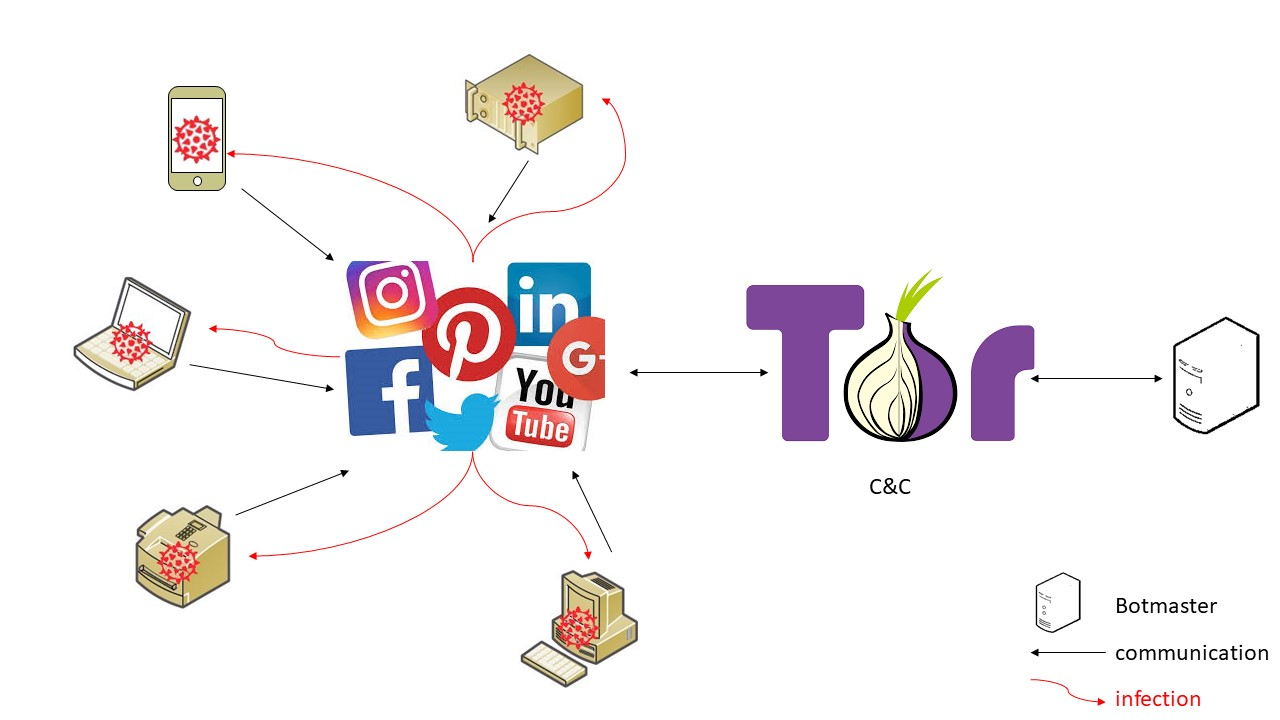
\includegraphics[width=0.75\textwidth]{reseau_aleatoire}
%	\label{fig:réseau_aléatoire}
%	\caption[Architecture aléatoire]{Architecture aléatoire}
%\end{figure}

\subsubsection{Définition}
Ce concept représente une variante de l'architecture centralisée et peut se retrouver dans une variété de malware connue sous le nom de RATs\footnote{Remote Access Trojan}.Ces chevaux de Troie fonctionnent sur un principe de client/serveur parfois mis en place avec des techniques de social engineering (exemple: un fichier d'installation récupéré sur un site douteux). Ils exécutent la partie client à l'insu de l'utilisateur pour se connecter au serveur.
\newline Cette architecture tire profit de l'exploitation de plate-formes existantes supportant le protocole HTTP comme Facebook, Twitter, Yahoo, Evernote, Google, etc. et de réseau permettant de camoufler les échanges comme TOR, Hornet, etc.

\subsubsection {Liste des protocoles utilisés par le botnet}
\begin{itemize}
	\item HTTP
	\item protocole propriétaire (exemple XMPP\footnote{Extensible Messaging and Presence Protocol de MSN Messenger})
	\item IRC
\end{itemize}

\subsubsection{Avantages}
\begin{itemize}
	\item Architecture déjà existante
	\item Réseau important en terme d'utilisateurs
	\item Utilisation des canaux existants (exemple: messagerie instantanée)
	\item utilisation des fonctionnalités du réseau (exemple :Le réseau anonymisation TOR)
	\item Difficulté de démanteler son propre réseau
\end{itemize}

\subsubsection{Inconvénients}
\begin{itemize}
	\item Vulnérabilité du botnet face aux mécanismes de défense
	\item Connexion en permanence
	\item bloqué par le filtrage de liens de la plate-forme
\end{itemize}

%--------------------------------------------------------------------
%ajouter un botnet
%glisser le .csv dans le dossier exemples de la section 2
%inclure la ligne \csvautotabular[respect all]{Section/2-Ssection/exemples/nom-du-botnet}
%--------------------------------------------------------------------


\subsubsection{exemples}


%\noindent
%\resizebox{\textwidth}{!}{
%\csvautotabular[respect all]{Section/2-Ssection/exemples/Cutwail.csv}
%}
%\resizebox{\textwidth}{!}{
%\csvautotabular[respect all]{Section/2-Ssection/exemples/Carna.csv}
%}




%Section-archi-centralise-Architecture_de_BOTNET


\subsection[Architecture  centralisée]{Architecture  centralisée}

%\begin{figure}[h]
%	\centering
%		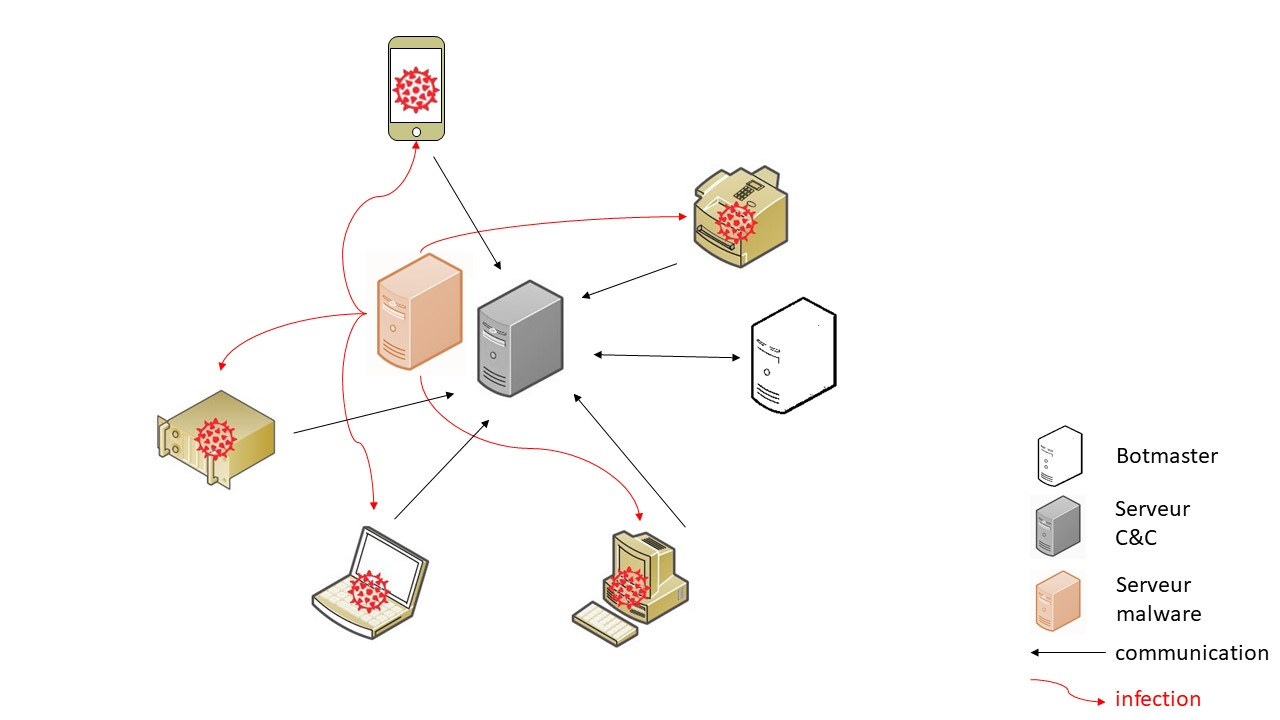
\includegraphics[width=0.75\textwidth]{archi_centralise}
%	\label{fig:archi_centralisée}
%	\caption[Architecture  centralisée]{Architecture  centralisée}
%\end{figure}


%\begin{figure}[h]
%	\centering
%		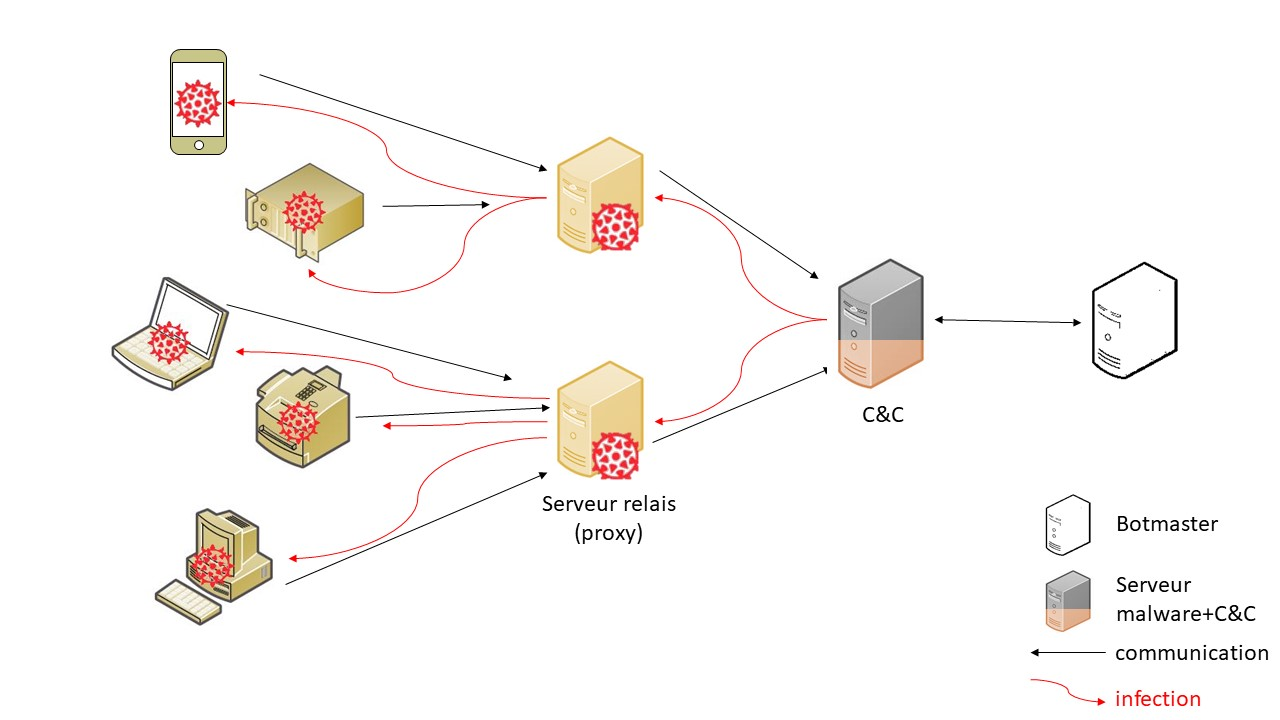
\includegraphics[width=0.75\textwidth]{archi_centralise_2}
%	\label{fig:Archi_centralisé_2}
%	
%	\caption[Architecture  centralisée répartie par utilisation d’une batterie de serveurs relais]{Architecture  centralisée répartie par utilisation d’une batterie de serveurs relais}
%\end{figure}

\subsubsection{Définition}
Un ou plusieurs nœuds de communication permettent aux bots d'échanger des données via un canal de communication.
Les nœuds représentent un serveur ou serveur relais avec comme fonction le C\&C.

\subsubsection{Liste des protocoles utilisés par le botnet}
\begin{itemize}
	\item IRC\footnote{Internet Relay Chat}
	\item HTTP\footnote{HyperText Transfer Protocol}
	\item IRC modifié
\end{itemize}

\subsubsection{Avantages}
\begin{itemize}
	\item Architecture  centraliséee
	\item Simplicité de mise en oeuvre (mIRC, ...)
	\item Utilisation des canaux IRC (topics, messages) pour l’envoi des commandes vers les botsPerformance (non gourmant en bande passante)
	\item Connexions régulières entre les bots et le C\&C (non-permanente)
	\item Recherche des ordres dans des forums, avec des mots clés ou même dans des images (stéganographie)
\end{itemize}

\subsubsection{Inconvénients}
\begin{itemize}
	\item Vulnérabilité du botnet (serveur central)
	\item Connexion en permanence
	\item Facile à détecter (filtrage du flux IRC)
\end{itemize}

%--------------------------------------------------------------------
%ajouter un botnet
%glisser le .csv dans le dossier exemples de la section 2
%inclure la ligne \csvautotabular[respect all]{Section/2-Ssection/exemples/nom-du-botnet}
%--------------------------------------------------------------------


%\subsubsection{exemples}
%\noindent
%\resizebox{\textwidth}{!}{
%\csvautotabular[respect all]{Section/2-Ssection/exemples/BEBLOH.csv}
%}
%\noindent
%\resizebox{\textwidth}{!}{
%\csvautotabular[respect all]{Section/2-Ssection/exemples/BOBAX-KRAKEN.csv}




%Section-archi-decentralise-Architecture_de_BOTNET


\subsection{Architecture décentraliséee}

%\begin{figure}[h]
%	\centering
%		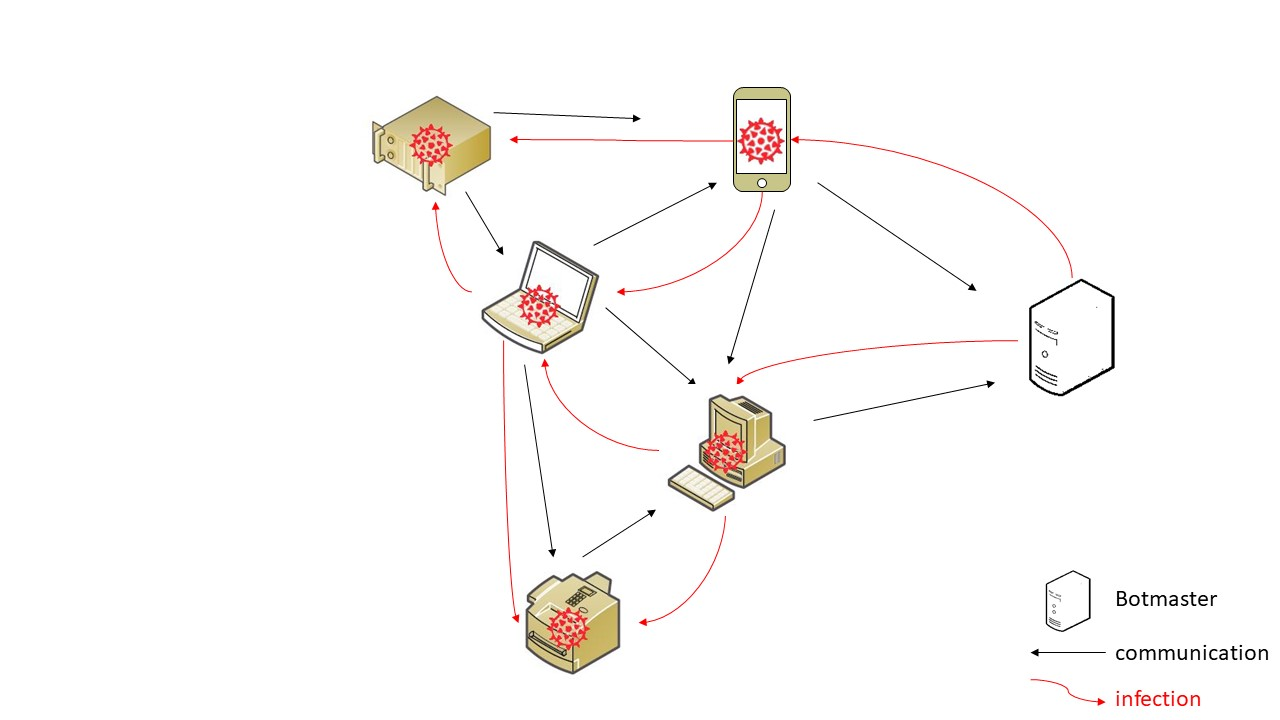
\includegraphics[width=0.75\textwidth]{P2P_non_structure}
%	\label{fig:P2P_non_structure}
%	\caption{P2P non structuré}
%\end{figure}
%\begin{figure}[h]
%	\centering
%		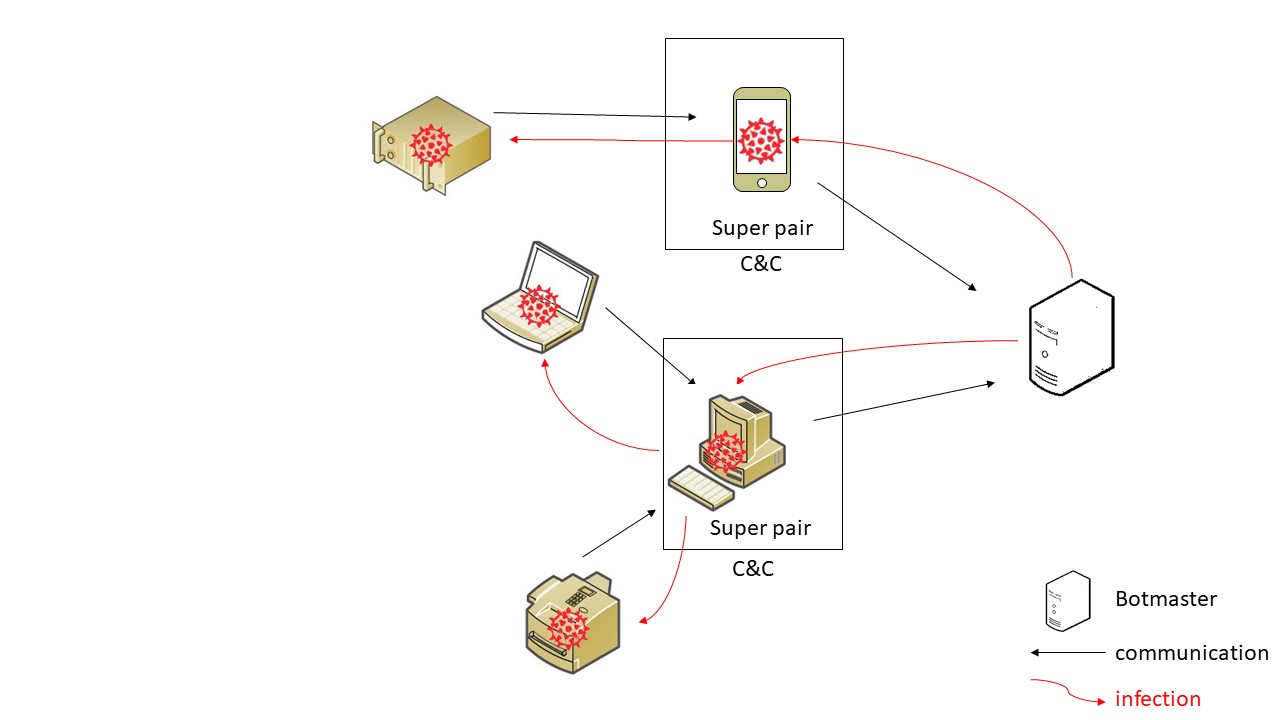
\includegraphics[width=0.75\textwidth]{P2P_avec_super_pairs}
%	\label{fig:P2P_avec_super_pairs}
%	\caption{P2P avec super-pairs}
%\end{figure}

\subsubsection{Définition}
\par En utilisant des réseaux peer-to-peer, on s’affranchit d'un point central de communication.Chaque bot, selon ses caractéristiques, apporte les ressources pour élaborer le système de C\&C.
Il existe plusieurs typologies de réseau overlay\footnote{réseau logique de recouvrement}:
\begin{itemize}
	\item \textbf{overlay P2P non-structuré} : les topologies sont aléatoires (loi de puissance, aléatoire uniforme,...)
  \item \textbf{overlay P2P par super-pairs} : tous les pairs du réseau ne sont pas égaux, certains d’entre eux étant automatiquement sélectionnés pour servir temporairement le rôle de serveur pour les recherches ou le contrôle du réseau (comme FastTrack ou Gnutella)
  \item \textbf{overlay P2P structuré} : une cartographie établissant le lien entre le contenu et son emplacement ; ce type de réseau implémente en général – mais pas systématiquement une table de hachage distribuée (DHT) ; on retrouve dans cette catégorie les protocoles P2P Chord, Tapestry et Kademlia (utilisé par le logiciel eMule).
\end{itemize}

\subsubsection{Liste des protocoles utilisés par le botnet}
\begin{itemize}
	\item TCP/IP
	\item UDP
\end{itemize}

\subsubsection{Avantages}
\begin{itemize}
	\item Architecture décentralisée
	\item Indépendant de l’architecture DNS
	\item difficile à repérer
	\item Connexions régulières entre les bots et le C\&C (non permanente)
	\item Le botmaster donne les informations comme un bot faisant partie du réseau
  \item L’information transite de voisin en voisin
	\item très difficile à neutraliser
\end{itemize}

\subsubsection{Inconvénients}
\begin{itemize}
	\item Pas de vision globale du réseau par un bot
	\item Connexion en permanence
	\item Facile à détecter (filtrage du flux IRC)
\end{itemize}

%--------------------------------------------------------------------
%ajouter un botnet
%glisser le .csv dans le dossier exemples de la section 2
%inclure la ligne \csvautotabular[respect all]{Section/2-Ssection/exemples/nom-du-botnet}
%--------------------------------------------------------------------

%\subsubsection{exemples}
%\noindent
%\resizebox{\textwidth}{!}{
%\csvautotabular[respect all]{Section/2-Ssection/exemples/Storm.csv}
%}
%\resizebox{\textwidth}{!}{
%\csvautotabular[respect all]{Section/2-Ssection/exemples/QAKBOT.csv}
%}

%Section-archi-hybride-Architecture_de_BOTNET
\subsection{Architecture hybride}

%\begin{figure}[h]
%	\centering
%		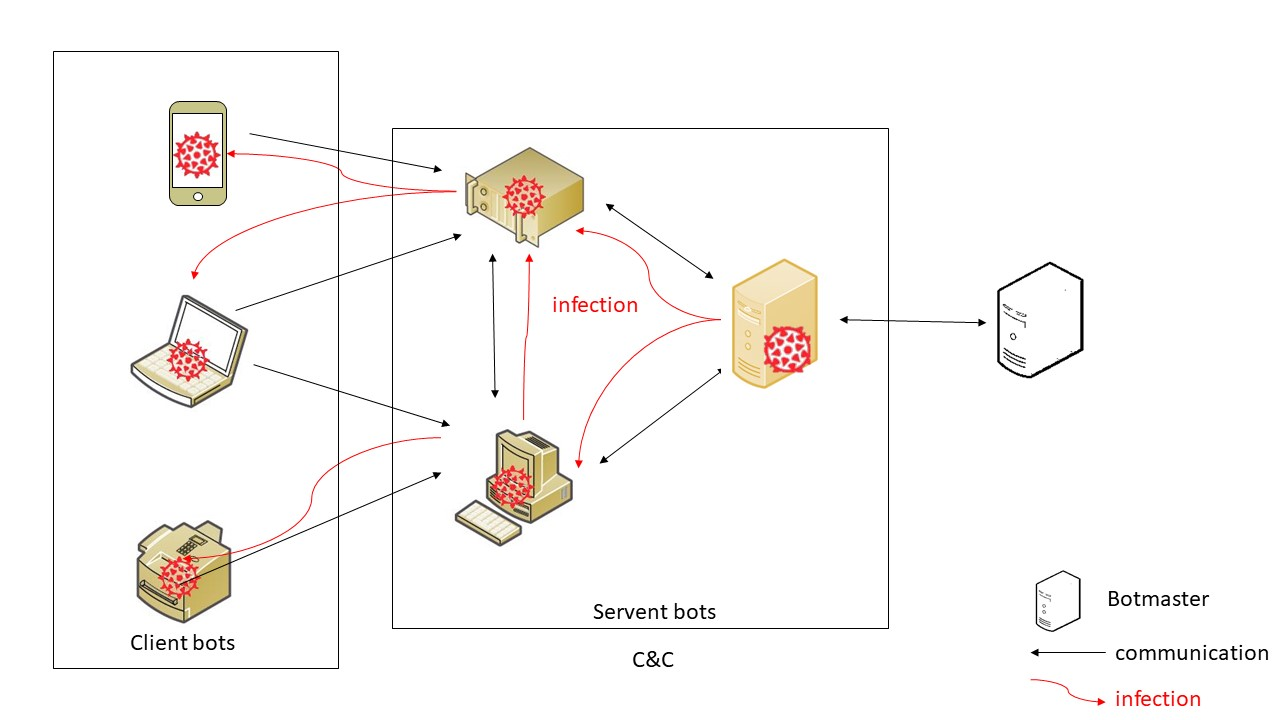
\includegraphics[width=0.75\textwidth]{structure_hybride_P2P}
%	\label{fig:structure_hybride_P2P}
%	\caption[Structure hybride P2P]{Structure hybride P2P}
%\end{figure}

\subsubsection{Définition}
Une architecture hybride intègre une solution de repli, comme à l'aide d'un DGA\footnote{Domain Generation Algorithm} ou de plusieurs niveaux successifs entre le P2P et le C\&C.Cette hiérarchie permet de masquer une partie des adresses IP utilisées afin de rendre plus complexe l'analyse du botnet.
L'association de bot clients et de bots servent\footnote{serv-\textbf{eur} et cli-\textbf{ent}} met en évidence l'organisation du réseau par le botmaster.
Ces niveaux intermédiaires permettent de solidifier l'architecture du réseau.

\subsubsection{Liste des protocoles utilisés par le botnet}
Reprenant les protocoles présentés dans les architectures précédentes, L'efficacité, la furtivité et la complexité des méthodes de communication ont pour objectif de nuire aux efforts de démantèlement.
Ainsi, les coopérations internationales entre acteurs institutionnels et
privés sont généralement nécessaires pour permettre de démanteler les botnets les plus sophistiqués.

\subsubsection{Avantages}
\begin{itemize}
	\item Nombre important de domaines
  \item masquage de l'adresse IP
\end{itemize}

\subsubsection{Iconvénients}
\begin{itemize}
	\item tributaire de la bande passante
\end{itemize}

%--------------------------------------------------------------------
%ajouter un botnet
%glisser le .csv dans le dossier exemples de la section 2
%inclure la ligne \csvautotabular[respect all]{Section/2-Ssection/exemples/nom-du-botnet}
%--------------------------------------------------------------------

\subsubsection{exemples}

%\noindent
%\resizebox{\textwidth}{!}{
%\csvautotabular[respect all]{Section/2-Ssection/exemples/Gameover-Zeus.csv}
%}
%\resizebox{\textwidth}{!}{
%\csvautotabular[respect all]{Section/2-Ssection/exemples/Mirai.csv}
%}

%$$$$$$$$$$$$$$$$$$$$$$$$$$$$$$$$$$$$$$$$$$$$$$$$

%Analyse-Architecture_de_BOTNET

\subsection{L'analyse} 
\subsubsection{L'analyse statique}
Réalisée en sandbox, sur une machine virtuelle ou une machine dédiée avec des outils pré-installés comme InetSim,FakeNet ou Mozzle, elle débute par une analyse statique pour identifier les éléments et la composition du malware.
L'examen du code et des fonctions appelées permettent d'évaluer les capacités du botnet.
\subsubsection{L'analyse dynamique} 
Cette étape est relativement utile pour la compréhension de la menace car elle présente la machine infectée sous plusieurs états à l'aide de snapshots\footnote{copie des données/modifications apportées à un système}.
Ces captures instantanées situent l'avancement de l'infection lors de l'attaque.
Il est souvent nécessaire en présence d'algorithme chiffré d'utiliser cette méthode pour désobfusquer le code et comprendre la structure du malware.


%Defense-et-blocage-Architecture_de_BOTNET

\subsection{La défense et le blocage}
Au même titre que la protection contre les malwares, les recommandations en terme de SSI\ulink{https://www.ssi.gouv.fr/administration/bonnes-pratiques/}{recommandations ANSSI}, applicables localement, doivent s'inscrire dans nos habitudes et augmentent ainsi la probabilité de bloquer l'étape initiale de l'infection (spam, navigation non-sécurisée,etc.).
\newline Les mises à jour logicielles et système sont essentielles pour bloquer l'exploitation de CVE\footnote{Common Vulnerabilities and Exposures} \ulink{https://www.cvedetails.com}{Common Vulnerabilities and Exposures}.
\newline Au niveau du FAI, les notifications en cas de connexions malveillantes et la surveillance des adresses IP sont un frein à l'extension du botnet.
\newline Enfin la détection d'un appel de fonctions anormales par l'antivirus, l'autorisation et l’identification des flux sortants par le firewall permettent le blocage de l'activité malveillante.
Les fonctionnalités recherchées de l'antivirus dans ce cadre sont un firewall bidirectionnel, une protection contre le phishing, la vérification de la certification, la lutte contre le tracking, la vérification du téléchargement, le blocage des pop-ups et pages WEB malveillantes,etc. 

%Demantelement-Architecture_de_BOTNET
\subsection{Le démantèlement}
Les méthodes de détection impliquent parfois des actions offensives visant à entraver le développement du botnet.
Il est cependant nécessaire d'avoir un support juridique et judiciaire pour mener à bien des actions adaptées au type et à la taille du botnet.
Celles-ci sont généralement menées en coopération avec les industriels (Microsoft,Level 3, Cisco,etc.) et la communauté scientifique.

%Detection-Architecture_de_BOTNET

\subsection{La détection}
Recherche d'anomalie, comparaison de signatures, pots-de-miel, toutes ces techniques basées sur l'activité du réseau reposent sur l'inspection des flux et des paquets.

\subsubsection{La détection passive}
L'identification et l'analyse passive des flux (adresses IP,port source et destination, étiquette MPLS\footnote{MultiProtocol Label Switching}, etc.) permettent de classifier les protocoles suspects et les serveurs de C\&C.
\newline BotFinder, par exemple, permet de décomposer un flux (durée moyenne des connexions, nombre d'octets transférés, etc.) et de le comparer à l'activité normale du réseau.
\newline L'observation des DNS\footnote{Domain Name Server} permet aussi d'identifier les domaines malveillants afin de caractériser le botnet suspecté.
BotGad, un système d'exploitation permettant d'analyser le trafic DNS sur un réseau local, utilise un algorithme basé sur l'apprentissage afin de définir la stratégie de groupe du botnet.
\newline EXPOSURE, un autre système d'exploitation déployé au sein de l'ISP\footnote{Internet Service Provider}, permet d'analyser à large échelle mais sur une durée de plusieurs mois le trafic DNS. Produisant une liste de domaines malveillants, il permet, par exemple, d'identifier un volume conséquent de requêtes pour un même domaine.
\newline Enfin le recours aux pots-de-miel et l'analyse des journaux d'activité sont les éléments de base d'une recherche d'activité liée aux botnets.
Suivant cette idée, le SIEM\footnote{Security Information and Event Management}, une solution de gestion de la sécurité, représente un outil précieux et novateur afin d'optimiser la veille du trafic et d'automatiser les processus de sécurité en cas de comportement anormal.

\subsubsection{La détection active}
Différentes techniques existent comme le sinkholing\footnote{également appelé serveur gouffre, gouffre Internet ou Blackhole DNS } redirigeant le trafic vers des serveurs afin de simuler le comportement du C\&C et de diminuer la puissance du réseau du botnet.
\newline L'infiltration, fonction de l'architecture du botnet, consiste à simuler le comportement d'un botnet contrôlé à l'aide de drones IRC ou de script afin de capturer le trafic et de remonter jusqu'au botmaster.
Le projet Pebbletrace reprend cette idée d’identification du botmaster en piégeant les équipements infectés avec une charge défensive afin de retourner le trafic contre le botnet.


%synthese
Les botnets font maintenant partie d'une économie souterraine sous forme de services payants.
Le harcèlement, le vol, les attaques par déni de service, etc figurent comme des produits de vente accessibles, moyennant finances, pour n'importe quel criminel.
\newline D'après l'ENISA\footnote{European Union Agency for Cybersecurity, anciennement European Network and Information Security Agency} les prix varient suivant la fiabilité, la durée et le type de service requis.
Par exemple une heure de DDoS est disponible pour 38\$.
Les différentes architectures permettent de mieux comprendre l'organisation du botnet et l'importance du C\&C.
\vspace{5mm}
\newline Les notions de veille technologique et de partage d'informations sur la menace sont essentielles du fait de l'implication du botnet dans les réseaux publiques et privés.
\newline Dans le cadre du renseignement lié aux menaces, les constructeurs de smartphone fournissent les informations (recherches, cibles des attaques, menaces associés aux mobiles, vulnérabilités des objets IoT) issues de leurs Threat Intelligence Center\footnote{Centre de renseignements liés aux menaces cyber}.
%ouverture
\vspace{5mm}
\newline Selon Nokia (\ulink{https://www.nokia.com/about-us/news/releases/2018/12/04/nokias-threat-intelligence-report-2019-warns-on-the-fast-growing-and-evolving-threat-of-malicious-software-targeting-internet-of-things-iot-devices/}{Nokia's Threat Intelligence Report}, l'activité des botnet sur l'IoT représente 78\% des événements de détection de malware en 2018.
\newline La menace omniprésente de ces objets connectés (santé, domotique, médias, électroménager,...) n'est aujourd'hui pas assez prise en considération par notre société de consommation.
Le manque de sécurité accrue de ces appareils fait apparaître ces objets connectés comme des acteurs potentiels constituant le réseau d'un botnet.
\newline L'arrivée prochaine de la 5G\footnote{prévisions en moyenne 100Mbit/S en download et 50 Mbit/s en upload} sera, dans ce domaine, un vecteur majeur pour la diffusion de l'infection du malware et le nombre d'attaques associés au botnet (exemple attaques DDoS).


%\begin{figure}[h!]
%\begin{center}
%	
\includegraphics[width =0.6\textwidth, keepaspectratio]{coverback}
%	\caption{Figure 1}\label{mon image}
%	\end{center}
%\end{figure}

\section{Malware}

\subsection{Malware industriel : citadel}

Les créateurs du malware Citadel ont adopté un modèle de développement Open Source qui leur permet de corriger collectivement les bugs et d'ajouter plus rapidement des fonctionnalités à leur logiciel malveillant. Citadel est basé sur ZeuS, l'un des plus anciens et des plus populaires Cheval de Troie mis au point pour pirater les services bancaires en ligne. Zeus a été abandonné par son créateur fin 2010, mais quelques mois plus tard, le code source de son malware a été diffusé sur le Net. Depuis la publication de son code source, Zeus a servi de base au développement d'autres Trojan comme Ice IX,  et Citadel. « Le 17 décembre 2011, pour la première fois, un laboratoire de recherche (Seculert) a mis en évidence l'existence d'un botnet Citadel, » a déclaré le spécialiste de la sécurité dans un blog. « Le taux d'adoption et le développement de ce malware est en pleine expansion. » Seculert dit avoir identifié plus de 20 réseaux de zombies utilisant des versions différentes du Cheval de Troie. « Chaque version comporte de nouveaux modules et de nouvelles fonctionnalités, certaines proposées par les clients de Citadel eux-mêmes, » a indiqué l'entreprise de sécurité. L'aspect le plus intéressant de ce malware est sans aucun doute le processus adopté pour son développement. Les modalités de développement adoptées pour Citadel ressemblent à celles des communautés supportant des projets Open Source. « L'organisation est calquée sur le développement des logiciels courants : les créateurs de Citadel fournissent à leurs clients un manuel utilisateur, des avis donnant des détails sur les mises à jour et même un contrat de licence.

%==========================
\chapter{Réagir et remédier}
\ulindex{incidents}

%-------------------------------------------------------------
%               FR CYBERDEF SECOPS COURSE
%                      INCIDENT MANAGEMENT
%
%                                    Introduction
%
%                              2020 eduf@ction
%-------------------------------------------------------------
%==================================================
\section{GERER les incidents}

La réponse aux incidents est une approche organisée pour traiter et gérer les conséquences d'une violation de la sécurité ou d'une cyberattaque, également appelée incident informatique ou incident de sécurité (informatique). L'objectif d'une réponse à incident est de gérer la situation de manière à limiter les dommages et à réduire le temps et les coûts de récupération des informations, et de reprise d'activité et de retour à la normale.

La réponse aux incidents de sécurité informatique est devenue un axe majeur de la gestion de la sécurité en entreprise. De nouveaux types d'incidents émergent régulièrement avec des manières d'agir et de réagir différents. Il est important de distinguer les incidents liés à des phénomènes accidentels à ceux liés à des atteintes intentionnelles. Nous distinguerons donc ici la notion d'incident de sécurité d'incident informatique, en nous concentrant sur le volet incident de sécurité considéré comme lié à des attaques informatiques.  
Les activités préventives basées sur les résultats des évaluations des risques peuvent réduire le nombre d'incidents de sécurité à impact, mais tous ces incidents ne peuvent pas être évités. Une capacité de réponse aux incidents de sécurité est donc nécessaire pour traiter rapidement les incidents, minimiser les impacts, réduire les pertes et destructions, couvrir les faiblesses qui ont été exploitées et restaurer les services numériques. 

Idéalement pour des attaques, les activités de réponse aux incidents sont menées par l'équipe de réponse aux incidents de sécurité informatique de l'organisation (\g{aCSIRT}) car elle nécessite des postures particulières.  L'équipe peut également comprendre des représentants des services juridique, des ressources humaines, de la communication, et des risques. L'équipe de réponse aux incidents suit normalement un plan de réponse aux incidents (\gls{aIRP}) de l'organisation, qui est un ensemble d'instructions écrites qui décrivent la réponse de l'organisation aux événements du réseau, aux incidents de sécurité et aux impacts confirmés. 

Cette réponse planifiée aux incidents est une entreprise complexe, l'établissement d'une capacité de réponse aux incidents réussie nécessite une planification et des ressources importante. La surveillance continue des attaques est essentielle en avant phase. Il est essentiel d'établir des procédures claires pour hiérarchiser le traitement des incidents, tout comme la mise en œuvre de méthodes efficaces de collecte, d'analyse et de communication des données. Il est également essentiel d'établir des relations et d'établir des moyens de communication appropriés avec d'autres groupes internes (par exemple, les ressources humaines, les services juridiques) et avec des groupes externes (par exemple, d'autres équipes de réponse aux incidents (CERT, CSIRT..), les forces de l'ordre).

L'établissement d'une capacité de réponse aux incidents doit comprendre les actions suivantes :

\begin{itemize}
  \item Création d'une politique et d'un plan de réponse aux incidents;
  \item  Élaboration de procédures pour effectuer le traitement et le signalement des incidents;
  \item Définir des lignes directrices pour communiquer avec des tiers sur les incidents;
   \item Sélection d'une structure d'équipe et d'un modèle de dotation;
  \item  Établir des relations et des voies de communication entre l'équipe d'intervention en cas d'incident et d'autres groupes, à la fois internes (par exemple, le service juridique) et externes (par exemple, les forces de l'ordre);
  \item Déterminer quels services l'équipe d'intervention devrait fournir en cas d'incident ;
  \item Recruter et former l'équipe d'intervention en cas d'incident.
\end{itemize}


Les organisations doivent généralement être prêtes à gérer tout incident, mais elles doivent se concentrer sur leur préparation à gérer les incidents qui utilisent des vecteurs d'attaque courants.
Les incidents peuvent se produire de nombreuses façons, il est donc impossible d'élaborer des instructions étape par étape pour gérer chaque incident. Cette publication définit plusieurs types d'incidents, basés sur des vecteurs d'attaque courants; ces catégories ne sont pas destinées à fournir une classification définitive des incidents, mais plutôt à être utilisées comme base pour définir des procédures de manipulation plus spécifiques. Différents types d'incidents méritent différentes stratégies d'intervention. 

Les vecteurs d'attaque les plus courants:

\begin{itemize}
  \item Support Media externe / amovible: attaque exécutée à partir d'un support amovible (par exemple, un lecteur flash, un CD) ou un périphérique;
  \item Attrition: attaque qui utilise des méthodes de force brute pour compromettre, dégrader ou détruire des systèmes, des réseaux ou des services;
  \item Web: attaque exécutée à partir d'un site Web ou d'une application Web;
  \item Courriel: une attaque exécutée via un message électronique ou une pièce jointe;
  \item Utilisation incorrecte: tout incident résultant d'une violation des politiques d'utilisation acceptables d'une organisation par un utilisateur autorisé, à l'exclusion des catégories ci-dessus;
  \item  Perte ou vol d'équipement: la perte ou le vol d'un appareil informatique ou d'un support utilisé par l'organisation, tel qu'un ordinateur portable ou un smartphone;
\end{itemize}


\subsection{Réponse à incident}
%--------------------------------------------------------------------------------

% https://searchsecurity.techtarget.com/definition/incident-response
La réponse sur incident de sécurité pose de nombreuses problèmes \g{d'opérationnalité} tant sur les aspects techniques que juridiques ou organisationnels. Dans ce chapitre, nous allons tenter d'aborder les différentes méthodologies et outils qui permettent de répondre aux enjeux de la réactivité en cas d'incident cyber. La réponse à incident, doit s'inscrire dans une organisation cohérente permettant de gérer l'ensemble de la chaîne de traitement d'un incident. On parle de \g{Gestion des incidents} (\textit{Incident Management}). Cette gestion des incidents est en outre à cheval entre les deux grands processus  de la SECOPS, la surveillance-détection et la  réponse à incident. Dans ce document nous nous focaliserons sur cette réponse à incident au sens du traitement d'un incident lié à une menace avérée ayant un impact sur les systèmes d'information, et non les évènements de sécurité qui ne réclament pas d'action immédiate. Ces derniers ne sont bien évidement pas à négliger.

Un événement est donc toute occurrence observable dans un système ou un réseau. Les événements incluent un utilisateur se connectant à un partage de fichiers, un serveur recevant une demande de page Web, un utilisateur envoyant un e-mail et un pare-feu bloquant une tentative de connexion. Les événements indésirables sont des événements ayant une conséquence négative, tels que les pannes du système, les inondations de paquets, l'utilisation non autorisée des privilèges système, l'accès non autorisé aux données sensibles et l'exécution de logiciels malveillants qui détruisent les données. Ce guide ne traite que des événements indésirables liés à la sécurité informatique, pas ceux causés par des catastrophes naturelles, des pannes de courant, etc.


Un incident de sécurité informatique est une violation ou une menace imminente de violation des politiques de sécurité informatique, des politiques d'utilisation acceptables ou des pratiques de sécurité standard ou simplement une menace active ayant un impact sur l'activité de l'entreprise, on peut citer des cas classiques comme :  Exemples d'incidents2:

\begin{itemize}
  \item Un attaquant pilote botnet pour générer un DDOS sur  un site WEB important de l'entreprise;
  \item Les utilisateurs sont amenés à ouvrir un document envoyé par e-mail contenant un malware ou utilisant une vulnérabilité pour exécuter un outil qui infecte leurs ordinateurs pour établir des connexions avec un hôte externe ou pour chiffrer des fichiers pour réclamer une rançon;
  \item Un attaquant obtient des données sensibles et menace que les détails soient rendus publics si l'organisation ne paie pas une somme d'argent désignée.
  \item Un utilisateur fournit ou expose des informations sensibles à des tiers via des services de partage de fichiers poste à poste, ou en utilisant des services non déclarés (Shadow IT)
\end{itemize}


%- - - - - - - - - - - - - - - - - - - - - - - - - - - - - - - - - - - - - - - - - - - - - - - - 
\subsection{Terminologie}

% FRAME beamer PRZ ------------------------------------
\mode<all>{\texframe
{La réponse à incident}
{quelques éléments de définition}
{%. . . . . . . . . . . . . . . . . . . . . . . . . . . . . . . . . . . . .
La réponse à incident est le processus qui permet de déployer les moyens nécessaires pour traiter un événement de sécurité classé comme incident de sécurité.
Un incident de sécurité peut être enregistré en provenance de systèmes de sécurité, de veille ou d'audit. Le besoin d'intervention peut être immédiat comme différé.
La réponse peut nécessiter des équipes de compétences larges comme expertes sur un domaine donné. L'intervention peut nécessiter des moyens techniques importants ou pas, et mettre en isolation tout ou partie d'un système d'information.
}} % end FRAME.........................................................




La \textbf{gouvernance} de la réponse aux incidents consiste à planifier à l'avance et  de disposer un plan d'opération avant qu'il ne soit nécessaire. Plutôt que d'être un processus axé sur l'informatique, il s'agit d'une fonction  globale qui permet à une organisation de prendre des décisions rapides avec des informations fiables dans un contexte où la continuité d'activité ou l'image de l'entreprise est menacée. Non seulement le personnel technique des services informatiques et de sécurité est impliqué, mais aussi des représentants d'autres aspects clés de l'entreprise. La réponse à incident  interpelle  dans son mode d'opération, la gestion des plans de continuité et de reprise d'activité, la gestion de crise,  l'interaction juridique et contractuelle  ainsi que la gestion des relations avec les services de l'état (CNIL, ANSSI, Police et Gendarmerie ...). 

Je vous propose quelques éléments de terminologie avec la correspondance anglo-saxonne afin de se repérer dans les usages et trouver de l'information pertinente lors de vos recherches sur Internet :


% FRAME beamer PRZ ------------------------------------
\mode<all>{\texframe
{La réponse à incident}
{Terminologie}
{%. . . . . . . . . . . . . . . . . . . . . . . . . . . . . . . . . . . . .
\begin{itemize}
		\item \edxdico{Investigations Numériques}{Digital Investigation};
		\item\edxdico{Analyse légale}{forensique (Inforensique)};
		\item \edxdico{CERT}{Computer Emergency Response Team};
		\item \edxdico{CSIRT}{Computer Security Incident Response Team};
		\item \edxdico{Gestion des Incidents}{Incident Management}.
\end{itemize}
}} % end FRAME.........................................................

\subsection{Définitions}

\begin{notebox}{Incident}
Un incident de sécurité, correspond donc à la conséquence d’un ou plusieurs évènements de sécurité ou un évènement de sécurité majeur. Pour un \textbf{événement}, il n'y a pas de conséquence alors que pour un \textbf{incident} il y a un impact sur l’un des critères de sécurité DICA (Disponibilité, Intégrité, Confidentialité, Auditabilité).
\end{notebox}

Cette distinction a toujours existé, en effet l'ISO/IEC 27001 l'a reprise de l'ISO TR 18044:2004 (aujourd'hui remplacée par l'ISO/IEC 27035) qui l'avait elle-même reprise de l'ISO TR 13335-2:1997. 


% FRAME beamer PRZ ------------------------------------
\mode<all>{\texframe
{La réponse à incident}
{Evènement de sécurité}
{%. . . . . . . . . . . . . . . . . . . . . . . . . . . . . . . . . . . . .
Concrètement, un événement peut donc être :

\begin{itemize}
  \item soit la découverte d’une vulnérabilité;
  \item  soit la constatation d’une non-conformité;
  \item soit une altération, une perte ou une atteinte à l’information;
  \item   soit une altération ou une perte d’un élément du système d’information, d’un élément de configuration du SI ou d’un actif non-IT;
  \item  soit un ensemble corrélé d'indicateurs avertissant d'un comportement non sollicité ou malveillant;.
\end{itemize}
}} % end FRAME.........................................................

Un événement peut donner lieu à un \textbf{traitement préventif} dans la mesure où aucun impact n'a été identifié, par exemple la découverte d’une vulnérabilité.
Un \textbf{incident donne quant à lui obligatoirement lieu} à un \g{traitement curatif } car un impact a été identifié.
Ce qui motive la requalification d’un événement en incident doit impérativement être basé sur une décision humaine en fonction d'une estimation de l'impact.
Néanmoins avant de s'engager dans la description des activités liées à la réponse à incident cybersécurité, je souhaitais évoquer les bonnes pratiques ITIL qui donnent des pistes sur l'organisation de la gestion d'incident. Il ne faut en effet pas considérer la réponse à attaque comme une activité que technique bien que l'urgence nécessite le plus souvent de passer outre les processus classiques de traçabilité.


\subsection{Sources Incidents}

Il existe différents types d'incidents de sécurité et des moyens de les classer. Ce qui peut être considéré comme un incident pour une organisation peut ne pas être aussi critique pour une autre. Tous les incidents ne proviennent pas de SIEM. En effet le déclenchement d'incident peut avoir différentes sources.
 %-------------------------------------------------------------------------
\mode<all>{\picframe{../Latex/Sources/EDU/Pictures/img-incident-cycle}{Les axes de la gestion des cyber-Incidents}{0.7}{lblincident-cycle}}
%-------------------------------------------------------------------------


% FRAME beamer PRZ ------------------------------------
\mode<all>{\texframe
{La réponse à incident}
{Incidents courants}
{%. . . . . . . . . . . . . . . . . . . . . . . . . . . . . . . . . . . . .
Voici quelques exemples d'incidents relativement courants:

\begin{itemize}
  \item Une attaque par déni de service distribué ( DDoS ) contre les services cloud critiques;
  \item  Infection par un logiciel malveillant ou un rançongiciel qui a chiffré des fichiers d'entreprise critiques sur le réseau de l'entreprise;
  \item Une tentative de phishing réussie qui a conduit à la divulgation d'informations personnelles identifiables des clients;
  \item Perte ou vol, d'un ordinateur portable non chiffré avec des informations sensibles;
  \item Découverte sur internet (Darkweb) de données sensibles appartenant à l'entreprise.
\end{itemize}
}} % end FRAME.........................................................



 %-------------------------------------------------------------------------
\mode<all>{\picframe{../Latex/Sources/EDU/Pictures/img-incident-sources}{Les axes de la gestion des cyber-Incidents}{0.8}{lblincident-sources}}
%-------------------------------------------------------------------------

%- - - - - - - - - - - - - - - - - - - - - - - - - - - - - - - - - - - - - - - - - - - - - - - - 
\subsection{Parcours}

% Source https://en.m.wikipedia.org/wiki/Computer_security_incident_management


% FRAME beamer PRZ ------------------------------------
\mode<all>{\texframe
{La réponse à incident}
{SANS Institute - Plan de réponse}
{%. . . . . . . . . . . . . . . . . . . . . . . . . . . . . . . . . . . . .
Selon le SANS Institute, la réponse est construite autour de six phases clés d'un plan de réponse aux incidents:

\begin{itemize}
  \item \textbf{Préparation}: préparer les utilisateurs et le personnel informatique à gérer les incidents potentiels en cas de survenance;
  \item \textbf{Identification}: déterminer si un événement peut être qualifié d'incident de sécurité.
  \item \textbf{Confinement}: limiter les dommages de l'incident et isoler les systèmes affectés pour éviter d'autres dommages;
  \item \textbf{Éradication}: rechercher la cause première de l'incident et suppression des systèmes affectés de l'environnement de production;
  \item \textbf{Récupération}: autoriser les systèmes affectés à réintégrer l'environnement de production et garantir qu'aucune menace ne subsiste.;
  \item \textbf{Leçons apprises}: remplir la documentation de l'incident, effectuer une analyse pour tirer des leçons de l'incident et potentiellement améliorer les efforts d'intervention futurs.
\end{itemize}
}} % end FRAME.........................................................


Nous allons toutefois explorer la  gestion de l'incident au quotidien sur la base de trois actions fondamentales qui dans l'ordre correspondent au niveau de maturité d'une entreprise en terme de réponse à incident :


% FRAME beamer PRZ ------------------------------------
\mode<all>{\texframe
{La réponse à incident}
{Evènement de sécurité}
{%. . . . . . . . . . . . . . . . . . . . . . . . . . . . . . . . . . . . .
\begin{itemize}
  \item \textbf{Réagir} : premier processus, si nous pouvons le nommer ainsi est  la réaction immédiate en cas d'incident. Une entreprise peu ou pas organisée commence par découvrir les techniques de réponse à incident par cette première action. Cette réaction peut être compléter par des mécanismes (juridiques) de \textbf{neutralisation} de la menace, ou par exemple le déploiement d'un EDR pendant la phase de crise.

  \item \textbf{Enquêter} : si la réaction pour réduire l'impact ou neutraliser l'attaque est au coeur de la réponse à incident, il est nécessaire de rapidement lancer l'analyse des causes et origines de l'incident. Ce domaine d'action qui regroupe l'analyse post-morten et le forensique.

  \item \textbf{Anticiper} : organiser ses mécanismes de réponse (moyens et compétences), intégrer le processus de réponse à incident Cyber dans les mécanisme ITIL de gestion des incidents, organiser une cellule de CSIRT.

\end{itemize}
}} % end FRAME.........................................................

%-------------------------------------------------------------------------
\mode<all>{\picframe{../Latex/Sources/EDU/Pictures/img-liovar-incidents}{Incidents}{0.6}{lblliovarincident}}
%-------------------------------------------------------------------------


Dans certains ouvrages, le cycle des gestions d’incidents informatiques  peut être  présenté  en sept phases : Préparation, Détection, Identification, Isolement, Éradication, Restauration et Activités Post-Incident. 

Il est important de différencier les phases de Détection et d’Identification des autres.  La première étape consiste à découvrir la présence d’une cyberattaque ce que j'ai présenté pour ma part dans la partie \g{Threat Detection}  alors que la deuxième est composée de l’ensemble des investigations et analyses forensiques permettant de déterminer le type d’attaque et son étendue, d’identifier l’ensemble des systèmes et comptes infectés, ainsi que de préparer un plan d’action pour répondre activement à la cyberattaque (Isolation, Éradication et Restauration). Ce sont ces phases que nous traiterons comme le processus de gestion des incidents.

%  					\begin{itemize}
%  							\item 	Mécanismes et processus
%  							\item 	compétences
%  							\item 		outils
%					\end{itemize}








%-------------------------------------------------------------
%               FR CYBERDEF SECOPS COURSE
%                      INCIDENT MANAGEMENT
%
%                                   Anticipation
%
%                              2020 eduf@ction
%-------------------------------------------------------------

%Sources Intressantes
%https://www.societybyte.swiss/2019/04/03/la-gestion-des-cyberattaques-au-sein-dune-grande-entreprise-quels-en-sont-les-defis/



%==================================================
\section{ANTICIPER}
%--------------------------------------------------------------------------------

\subsection{Les bons reflexes}

Anticiper la réponse à incident, c'est s'organiser pour assurer rapidement un certain nombre d'actions rapides :

\begin{itemize}
  \item Conduire une levée de doute rapide pour s'assurer qu'il ne s'agit pas de faux positifs.   \item Mobiliser une équipe d'investigation afin de déterminer la cause de l'incident, d'identifier les vecteurs d'infection et de propagation de l'attaquant,
  \item Qualifier les impacts immédiats et à venir, construire un plan de défense le cas échéant ;
  \item Mettre en sûreté des systèmes critiques (cœur de confiance serveur de sauvegarde, etc.) qui seront nécessaires pour assurer la survie métier en particulier en cas d'incident lié à un impact destructeur comme les rançons logiciel activer les plans de contournement et des procédures en mode dégradé 
  \item et enfin mobiliser surtout les bonnes compétences, notifier les agences et les régulateurs et déclencher le cas échéant les assurances Cyber.
\end{itemize}

Cela ne s'improvise pas, et nécessite d'avoir structuré sa réponse à incident.

%==================================================
% 											MANAGEMENT DES INCIDENTS
%--------------------------------------------------------------------------------
\subsection{Etablir un processus de management} 
%--------------------------------------------------------------------------------


% https://csrc.nist.gov/publications/detail/sp/800-61/rev-2/final

\subsubsection{Résilience}
 
 On ne peut pas parler de réponse à incident dans un contexte d'attaque informatique sans parler de résilience.
 
La cyber-résilience ou la résilience numérique est la capacité d’un système d’information à résister à une panne ou une cyberattaque et à revenir à son état initial après l’incident, ou bien comme la faculté d’une structure quelconque à retrouver ses propriétés initiales après une altération significative. La notion peut s’appliquer aussi bien à un système physique ou un système d'information, qu’à un individu ou une organisation. 

Elle se traduit pour cette organisation par sa capacité de continuer à fonctionner et de résister à des agressions internes comme externes, volontaires ou non.

 Le niveau de résilience se mesure  avec des critères tels que la structure de l’organisation mise en place, les ressources humaines consacrées au fonctionnement du système, la redondance et le durcissement des systèmes et des équipements, les procédures en place, des compétences acquises à travers une formation et un entraînement dédiés, la connaissance fine de l’état de fonctionnement du système et la capacité à diagnostiquer une défaillance potentielle.
 
Sur le cyber-espace, la cyber-résilience implique donc de se préparer et de prendre  les mesures adaptées pour assurer le rétablissement d’un système. Par  ailleurs, dans le monde cyber dans l'entreprise l’incertitude peut régner dans l'usage :
\begin{itemize}
  \item  sur la sécurité des systèmes (virus déployés dont les effets ne sont pas maîtrisés), 
   \item l’intégrité du système n’est plus garantie, 
  \item l’activité du système peut être dégradée (données corrompues ou altérées) ou inopérante (communications inactives), 
  \item les risques de propagation des menaces sont augmentés si les interconnexions entre systèmes restent ouvertes, 
    
\end{itemize}

 Cette résilience peut  nécessiter des bascules vers des modes dégradés, avec l'isolation ou l'arrêt de certains sous-systèmes. Ce type de décision nécessite un circuit de décision rapide et court.

C'est dans un cadre de cette continuité d'activité que se situent la majorité des référentiels de management de l'incident de de sécurité.

\begin{notebox}{Résilience et continuité d'activité}
La capacité d’un système  à résister à une panne ou une cyberattaque et à revenir à son état initial après l’incident sera indifféremment appelé dans c\ecours résilience ou continuité d'activité. 
\end{notebox}


\subsection{L'intégration dans la gestion des incidents ITIL}

ITIL (\g{Information Technology Infrastructure Library} pour \g{Bibliothèque pour l'infrastructure des technologies de l'information}) est un ensemble d'ouvrages recensant les bonnes pratiques (\g{best practices}) du management du système d'information. 

La Gestion des incidents vue du côté d'ITIL  inclut tout événement qui perturbe, ou pourrait perturber, un service. Ceci inclut les événements communiqués directement par les utilisateurs, via le Centre de services, une interface web ou autrement.
Ce processus appartient au sens ITIL à l'étape Service Operation (SO) du cycle de vie d'un SI.

Même si les incidents et les demandes de service sont rapportés au Centre de services, cela ne veut pas dire qu'ils sont de même type. Les demandes de service ne représentent pas une perturbation de service comme le sont les incidents. Voir le processus Exécution des requêtes pour plus d'informations sur le processus qui gère le cycle de vie. 

Les objectifs du processus de Gestion des incidents sont :

\begin{itemize}
  \item Veiller à ce que des méthodes et des procédures normalisées soient utilisées pour répondre, analyser, documenter, gérer et suivre efficacement les incidents.
  \item  Augmenter la visibilité et la communication des incidents à l'entreprise et aux groupes de soutien du SI.
  \item  Améliorer la perception des utilisateurs par rapport aux TI via une approche professionnelle dans la communication et la résolution rapide des incidents lorsqu'ils se produisent.
  \item Harmoniser les activités et les priorités de gestion des incidents avec ceux de l'entreprise.
  \item Maintenir la satisfaction de l'utilisateur avec la qualité des services du SI.
\end{itemize}

Généralement, cette gestion d'incident s'inscrit dans une chaîne d'outillage avec des processus permettant de définir l'état ou le statut de l'incident.

\begin{itemize}
  \item \textbf{Nouveau} : un incident est soumis, mais n'a pas été assigné à un groupe ou une ressource pour résolution.
  \item \textbf{Assigné} : un incident est assigné à un groupe ou une ressource pour résolution.
  \item \textbf{En traitement }: l'incident est en cours d'investigation pour résolution.
  \item \textbf{Résolu} : une résolution a été mise en place.
  \item \textbf{Fermé} : la résolution a été confirmée par l'utilisateur comme quoi le service normal est rétabli.
\end{itemize}


% FRAME beamer PRZ ------------------------------------
\mode<all>{\texframe
{La réponse à incident}
{ITIL}
{%. . . . . . . . . . . . . . . . . . . . . . . . . . . . . . . . . . . . .
On ne peut toutefois pas oublier, que la gestion de la sécurité dans une entreprise mature, doit s'intégrer aux processus IT de l'entreprise et de remarquer que certaines activités de sécurité peuvent aussi s'intégrer dans un respect du référentiel ITIL.

\begin{itemize}
  \item Le centre de services (service desk) cf le niveau 1 d'un \g{Security Operation Center};
  \item La gestion des incidents (incident management) ;
  \item La gestion des problèmes (problem management) ;
  \item La gestion des changements (change management) voir  les mécanismes de couverture de vulnérabilités (patch management par exemple);
  \item La gestion des mises en production (release management) ;
  \item La gestion des configurations (configuration management).
\end{itemize}
}} % end FRAME.........................................................

Dans ces processus le cycle de vie de l'incident suit un cycle connu et reconnu : 

\begin{itemize}
  \item \textbf{Identification} : détecter ou rendre compte d’un incident ;
  \item \textbf{Enregistrement} : les incidents sont enregistrés dans le système de gestion des incidents ;
  \item \textbf{Classement}  : les incidents sont classés par priorité ;
  \item \textbf{Priorisation} : l’incident est classé par ordre de priorité, sur la base de son impact et de son urgence, pour une meilleure utilisation des ressources et du temps disponible par l’équipe de support ;
  \item \textbf{Escalade}  : l’équipe de support doit-elle obtenir de l’aide de la part d’un autre service ? Si oui, on engage une procédure de demande de service sinon, la résolution de l'incident s’effectue au niveau du support initial.
  \item \textbf{Diagnostic}  : révélation du symptôme complet de l’incident ;
  \item \textbf{Résolution et rétablissement } : une fois que la solution est trouvée et que la correction est apportée alors l’incident est résolu. La solution peut alors être ajoutée à la base des erreurs connues dans l'optique de résoudre plus rapidement un incident similaire dans le futur.
  \item \textbf{Clôture de l’incident}  : l’enregistrement de l’incident dans le système de gestion du management est clôturé en appliquant le statut « terminé » à celui-ci.
\end{itemize}


Les standards de gestion d’incidents (NIST 800-61 et ISO/IEC 27035) recommandent d’isoler les systèmes infectés directement après leur détection ce qui n'est pas toujours facile en contexte opérationnel. Cependant,  avec des APT, il doit être supposé que de nombreux systèmes informatiques peuvent avoir été compromis.  Ainsi, un confinement trop précoce sans analyse concrète de cette présence aura pour conséquence unique d’informer le cyber-criminel qu'il est potentiellement découvert. Le cyber-attaquant pourra donc réagir et prendre des contre-mesures telles qu’installer de nouveaux logiciels malveillants, détruire les traces numériques liées à son attaque (méthodes anti-forensiques) ou encore endommager l’environnement. Il faut donc dans la mesure du possible identifier intégralement la menace avant d’isoler les systèmes infectés et d’éradiquer les souches malveillantes.

 \subsection{La gestion des incidents avec l'ISO 27035}
 
 %https://pecb.com/en/education-and-certification-for-individuals/iso-iec-27035
 
 
 % FRAME beamer PRZ ------------------------------------
\mode<all>{\texframe
{La réponse à incident}
{avec l'ISO 27035}
{%. . . . . . . . . . . . . . . . . . . . . . . . . . . . . . . . . . . . .
 La mise en place d'un processus de gestion d’incidents, qu'il soit totalement intégré à la DSI via ITIL, ou des processus ISO9001 est complexe en entreprise mais les enjeux sont toujours identiques :
\begin{itemize}
  \item  Améliorer la sécurité de l’information;
  \item  Réduire les impacts sur le business;
  \item  Renforcer la prévention d’incident;
  \item  Assurer le recevabilité des preuves;
  \item  Mettre à jour l’appréciation des risques;
  \item  Prévention et sensibilisation.
\end{itemize}
}} % end FRAME.........................................................

  C'est ce que l'on retrouve dans l'ISO 27035, une norme de l'ISO qui structure  une organisation sur la réponse à incident autour d'une \textbf{politique} de gestion des incidents de sécurité.

Ce document de politique définit les éléments structurants. Il doit être pragmatique et adapté aux enjeux et à la taille de l’entité. Une bonne appropriation de cette  politique par les salariés est indispensable. 

La norme donne un guide  des incontournables de ce document :

\begin{itemize}
  \item Organisation générale (rôles et responsabilités, processus, équipes internes et externes, service de l'état, régulateurs ou agences nationales,... );
  \item Grandes définitions  (en particulier événement, incident, alerte et vulnérabilité);
  \item Sources (techniques, informationnelles et humaines) de remontée d’événements;
  \item Catégorisation et priorisation des incidents suivant des critères à préciser;
  \item Analyse post-mortem et analyse des retours d’expérience;
  \item Activation et fonctionnement de la cellule de réponse aux incidents (CSIRT - Cybersecurity Incident Response Team) comprenant les modalités de notification des incidents majeurs et d’activation de la cellule de crise.
  \item Sensibilisation des collaborateurs et formations dédiées.
\end{itemize}

Les phases de qualification et de décision reposent sur des expertises techniques très diverses en fonction des incidents.

Se lancer dans la construction d'un processus de gestion des incidents en interne ou pour un client en mode service, il est important d'être conscient des expertises nécessaire pour opérer :

Les \textbf{expertises techniques} liées à la \textbf{\g{surveillance détection}} qui s’appuient sur les solutions et équipements disponibles (IPS/IDS : intrusion detection / Prevention System, Security Information and Event Management : SIEM, logs locaux, analyseurs réseaux, supervision…), les clients,  partenaires et fournisseurs (CERT : Computer Emergency Response Team privés ou étatiques, opérateurs...).

Les expertises dépendent des caractéristiques techniques et fonctionnelles \textbf{des systèmes d’information} (technologies, logiciels, architectures, services cloud...). Le niveau de compétences des équipes internes ou externes qui assurent la maintenance conditionne la qualification  d’un événement dit incident. 

Des \textbf{expertises  plus orientées vers la réaction }pour traiter la réaction nécessitent des expertises pointues en sécurité (analyse du mode de propagation d’un code malveillant, analyse « forensique » d’un poste de travail  compromis…).

Le \textbf{niveau de capacité de support technique }ou de gestion de crise (Helpdesk) détermine le temps et la qualité de la réaction à l’incident et sa capacité de limiter les impacts. Les mauvaises décisions prises dans l’urgence pendant un incident sont souvent dûes à un manque d’expertise ou d’organisation dans la phase d'organisation de ces plans de réaction à incidents. Ces mauvaises décisions peuvent amplifier les impacts de l’incident voire faire basculer l’entité en crise.

Le  champ d’application de la norme est une approche planifiée et structurée :
\begin{itemize}
  \item De la détection, de l'analyse et du reporting des incidents de sécurité,
  \item De la réponse et du management des incidents de sécurité,
  \item De la détection, de l’analyse et du management des vulnérabilités de la sécurité de l’information,
  \item De l’amélioration continue de la sécurité de l’information et de la gestion d’incident, dans le cadre plus global du management de « l’incidentologie » et des vulnérabilités.
\end{itemize}


\subsection{Et avec la NIST 800-61}


Ce référentiel du NIST dénommé \g{Computer Security Incident Handling Guide} donne des recommendations interessante. Contrairement au normes ISO, l'intérêt des documents de NIST c'est qu'ils sont accessibles et concrets. \ulink{https://csrc.nist.gov/publications/detail/sp/800-61/rev-2/final}{GUIDE 800-61}

Entre ISO 27035 et NIST 800-61, Les deux normes fondent la gestion des incidents sur une approche cyclique assez comparable : 

Cycle de gestion des incidents dans NIST SP 800-61:

\begin{itemize}
  \item Préparation
  \item Détection et analyse
  \item Confinement, éradication et récupération
  \item Activité post-incident
\end{itemize}

Cycle de gestion des incidents dans ISO / IEC 27035:

\begin{itemize}
  \item Planifier et préparer
  \item Détection et signalement
  \item Évaluation et décision
  \item Réponses
  \item Leçons apprises
\end{itemize}

Les deux normes fournissent des recommandations détaillées sur l'équipe d'intervention en cas d'incident et les politiques et procédures de gestion des incidents. À mon avis, ces deux éléments sont essentiels pour une gestion efficace des incidents - pas les outils techniques. Donc, si vous commencez à développer des capacités de gestion des incidents dans votre organisation, concentrez-vous d'abord sur ces deux. Des procédures opérationnelles standard constamment améliorées aideront votre équipe à être efficace. Ils peuvent également aider à automatiser une partie des tâches.
Le NIST 800-61 propose une liste de contrôle de gestion des incidents, avec 9 phases simple à appréhender. Cette liste de contrôle est le premier stade de ce qui doit être maitrisé, et les personnes en charge de réponses aux incidents doit savoir comment exécuter les étapes contenues dans cette liste.
L'ISO / CEI 27035  se concentre davantage sur une organisation elle-même que les bonnes pratiques et le partage. 
C'est la combinaison des deux qui permet de se préparer correctement.
Je conseille aussi la lecture d'un document assez ancien (décembre 2006) mais intéressant pour organiser une petite équipe issu de l'ENISA \ulink{https://www.enisa.europa.eu/publications/csirt-setting-up-guide-in-french}{Guide de création d'un CSIRT pas à pas}

\subsection{Continuité d'activité  avec l'ISO 22301}

Autour de la gestion de la résilience, il existe un cadre normatif qui permet d'organiser les plans de continuité d'activité qui sont le pendant opérationnel  de la DSI de la gestion de l'incident de cybersécurité.
 La vocation des plans de continuité d’activité (Business Continuity Plans) est donc de répondre à des situations critiques, souvent  rares mais pouvant avoir des impacts graves pour l'entreprise.  Ces plans prennent en compte (inondation, incendie, accident industriel), on  intègre de plus en plus souvent des risques de conflit social, des attaques cyber de grande ampleur, des ruptures de service d’un prestataire  ou sous-traitant. La démarche pour concevoir son système de management de la continuité d’activité est l’objet de la norme ISO 22301. Une étape initiale consiste à analyser les impacts métiers (Business Impact Analysis) pour identifier les activités critiques et les besoins de reprise. La norme ISO 22317 fournit un cadre et des bonnes pratiques pour réaliser cette analyse.
 La norme ISO 22301 est intitulée « Sécurité sociétale — Systèmes de management de la continuité d'activité — Exigences ». Elle constitue un outil des organisations « pour anticiper et gérer la continuité de leurs activités » et « délivre des lignes directrices pour la mise en place d’un système de management spécifique et efficace  ». Elle a été publiée dans sa première version en 2012, puis révisée en 2019. Cette norme remplace des standards qui étaient jusque-là nationaux, comme celui par exemple britannique (BS-25999).
 
 
 En effet, lorsque toutes les stratégies de défense ont échoué et que la crise survient il est important de définir une cadre de résilience :    Comment l'entreprise peut-elle continuer à fonctionner, rétablir ses activités le plus rapidement possible et essayer de minimiser son impact ?
 
 C’est pour répondre à ces questions que  cette norme ISO 22301 a été construite.  Aujourd’hui encore, de nombreuses PME qui subissent une cyberattaque incapacifiante ne survivent pas . C’est  souvent  par un manque de en place d'une gestion de la continuité d’activité. La cyber résilience  encore un parent pauvre de la cybersécurité, non pas le manque travaux, mais simplement pas la non prise de conscience du risque de rupture totale de l'activité par des attaques informatiques.

% TODO  relecture

 La norme ISO 22301 se fixe comme objectif  de spécifier les exigences pour planifier, établir, mettre en place et en œuvre, contrôler, réviser, maintenir et améliorer de manière continue un système de management documenté afin de se protéger des incidents perturbateurs, réduire leur probabilité de survenance, s'y préparer, y répondre et de s'en rétablir lorsqu'ils surviennent. 

En résumé, elle aide les organisations « à se montrer mieux préparées et plus solides face à des interruptions de toutes sortes »  grâce notamment à la création d’un système de management de la continuité d’activité. Ce système de management de la continuité permettra également de s’assurer que les objectifs de la continuité soient alignés avec ceux de l’entreprise et de la direction .

Cette norme a été rédigée de façon générique pour englober le plus de situations possibles et pouvoir être appliquée dans des organisations de tous types et de toutes tailles . Les exigences spécifiées dans la norme le sont de manière « relativement brève et concise »  afin de pouvoir servir de base pour la certification. Pour avoir un peu plus de détaille, vous pouvez consulter la norme ISO 22313 donne les bonnes pratiques de la Continuité d’activité.



%-------------------------------------------------------------
%               FR CYBERDEF SECOPS COURSE
%                      INCIDENT MANAGEMENT
%
%                                      Reaction
%
%                              2020 eduf@ction
%-------------------------------------------------------------

\section{REAGIR}


%========================================================
% 											MANAGEMENT DES INCIDENTS
%-----------------------------------------------------------------------------------------
\subsection{La gestion de l'incident au quotidien} 
%--------------------------------------------------------------------------------

%- 1 - - - - - - - - - - - - - - - - - - - - - - - - - - - - - - - - - - - - - - - - - - - - - - 




\subsubsection{De l'alerte à l'incident}



Comme nous avons vu dans le chapitre sur la détection des attaques certains événements peuvent conduire à des alertes. Le terme alerte est ici synonyme d'alarme.  Ces alertes  doivent être analysées par des  analystes (Ingénieur SOC par exemple) pour caractériser si un événement ayant atteint à un niveau d'alerte doit être traité comme un incident de sécurité. L'alerte positionne les équipes dans un état de vigilance toutefois l'enregistrement d'un événement en incident engage les processus de réponse à  incident.
La question majeure est de savoir qui  mobiliser pour gérer l'incident. A l'image d'une alarme incendie, l'analyse de l'évènement qui à lever cette alarme doit être rapidement effectuée afin de valider l'événement comme devant être pris en charge par un processus dédié. 
Ce processus de vérification, est important pour éviter des FAUX POSITIF qui risquent de mobiliser des équipes de manière inadaptée.

Tout incident qui n'est pas correctement confiné et traité peut, et généralement, dégénérer en un problème plus important qui peut finalement conduire à une violation de données dommageable, à des dépenses importantes ou à l'effondrement du système. Une réponse rapide à un incident aidera une organisation à minimiser les pertes, à atténuer les vulnérabilités exploitées, à restaurer les services et les processus et à réduire les risques que posent les incidents futurs.
 
%TODO Insérer un schéma de traitement de l'incident

%- 1 - - - - - - - - - - - - - - - - - - - - - - - - - - - - - - - - - - - - - - - - - - - - - - 
\subsubsection{L'incident}

La problématique de la réaction à un incident dit \g{cyber} c'est que ce type d'incident  peut mettre en doute la confiance que l'on peut avoir dans son propre système système d'information. Comme ce SI risque d'être utiliser dans les mécanismes pour opérer la réaction, il est aussi important de gérer les critères de confiance et d'usage en mode dégradé.
Dans un premier dans nous allons donc partir de principe que le système d'information dispose de mécanisme permettant d'avoir confiance dans les systèmes qui opèrent pendant la réponse à incident.
Nous allons aborder la réaction à incident suivant les 3 volets  :
\begin{itemize}
  \item Remédier et reconfigurer pour limiter l’impact;
  \item  Enquêter sur l’incident;
  \item Neutraliser les sources de menaces;
\end{itemize}


Il est à noter que la norme donne des éléments d'organisation mais manque d'aspect pratique avec par exemple des fiches reflexes.

\subsubsection{Priorisation de l'évènement}
 Comme un événement est un changement observable du comportement normal d'un système, d'un environnement, d'un processus, d'un flux de travail, il est important de classifier ce changement dans un mécanisme de priorisation.  Il existe trois types de classification de base:
 
\begin{itemize}
  \item  \textbf{Normal}: un événement normal n'affecte pas les composants critiques ni ne nécessite de contrôle des modifications avant la mise en œuvre d'une résolution. Les événements normaux ne nécessitent pas la participation du personnel supérieur ou la notification de la direction de l'événement.
\textbf{Escalade} - un événement escaladé affecte les systèmes de production critiques ou nécessite la mise en œuvre d'une résolution qui doit suivre un processus de contrôle des modifications. Les événements escaladés nécessitent la participation du personnel supérieur et la notification des parties prenantes de l'événement.
\textbf{Urgence} - une urgence est un événement qui peut :
\begin{itemize}
  \item avoir un impact sur la santé ou la sécurité humaine;
  \item enfreindre les contrôles primaires des systèmes critiques ou sensibles de l'entreprise;
  \item affecter matériellement les performances des composants ou en raison de l'impact sur les systèmes de composants empêcher les activités qui protègent ou peuvent affecter la santé ou la sécurité des individus;
  \item être considéré comme une urgence par la politique de sécurité de l'entreprise .
\end{itemize}

\end{itemize}

%-------------------------------------------------------------------------
\mode<all>{\picframe{../Latex/Sources/EDU/SRC1/Pictures/img-mtbf}{Incidents}{0.8}{lblmtbf}}
%-------------------------------------------------------------------------


\subsection{Remédiation}

% Ajouter des éléments sur la 22301

Une question qui se pose lors d’une reprise d’activité est la confiance que nous avons dans le système. La difficultés après une attaque informatique ou une compromission, ou tout simplement une suspicion c’est la simple question de savoir si nous savons enlever toute la source de l’attaque. Reste-t-il des résidus.

\subsection{Aspect juridique de la réaction}

\utodo


%-------------------------------------------------------------
%               FR CYBERDEF SECOPS COURSE
%                      INCIDENT MANAGEMENT
%
%                                    Investigation
%
%                              2020 eduf@ction
%-------------------------------------------------------------

%========================================================
% 											ENQUETER
%-----------------------------------------------------------------------------------------
%==================================================
\section{ENQUETER}
%--------------------------------------------------------------------------------
%- - - - - - - - - - - - - - - - - - - - - - - - - - - - - - - - - - - - - - - - - - - - - - - - 
\subsection{Analyse de l'attaque}
Les enquêtes sur les intrusions visent à vérifier les modes d’attaque à l’œuvre dans les cyber-incidents, à déterminer les activités réseau postérieures aux événements, et à détecter les points terminaux et les comptes utilisateurs additionnels qui ont été compromis. Il est essentiel à la tenue d’une enquête sur une intrusion de tenter de comprendre l’étendue potentielle d’un incident.

\subsection{Evaluation détaillée des dommages}

Les évaluations des dommages consistent pour l’essentiel à identifier les données qui ont été infiltrées ou exposées, ainsi qu’à tenter de comprendre les motivations des cyber-adversaires et la suite possible des événements. Les évaluations peuvent mettre en lumière des enjeux qu’il importe de soulever et renseigner votre entreprise sur les conséquences éventuelles de la perte, de la fuite ou de l’exfiltration de données.


%\subsection{Se préparer et s'entrainer}


\subsection{forensique}

%source : https://www.algosecure.fr/conseil/investigation-forensique


\subsubsection{Cadre juridique}

L'analyse forensique est une science qui s'intéresse à la recherche de preuves sur des supports numériques pour comprendre un comportement, remédier à un incident et aider à prendre des décisions éclairées. Ces preuves sont des traces, des artéfacts numériques qui fournissent des informations qui, mises bout-à-bout, permettent de dégager un scénario factuel d'évènements et d'apporter des réponses aux questions que peut se poser le demandeur. L'analyse forensique est encore appelée investigation numérique, digital forensiques, inforensique ou informatique légale.


Dans une affaire judiciaire impliquant des supports numériques perquisitionnés pour des enquêtes, le juge peut faire appel à un expert judiciaire pour "faire parler" ces supports, pour l'aider dans sa prise de décision. L'expert judiciaire est une personne physique ou morale, professionnelle dans un domaine technique particulier, spécialement habilitée à exercer son expertise dans des dossiers judiciaires sur sollicitation d'un juge. Son avis ne s'impose pas au juge, qui reste libre dans l'appréciation des éléments fournis.


\subsubsection{Cadre non-juridique}

C'est ce que l'on retrouve le plus souvent avec les entreprises dans un contexte de réponse à incident à la suite d'une attaque du système d'information. Le cas plus fréquent est par exemple l'infection par un ransomware du parc d'une entreprise.

Dans ce type de situation aussi, il y a des sujets sur lesquels se focalisent les analystes en fonction des souhaits du client. Il peut s'agir de trouver qui a fait quoi, comment et quand, et à l'aide de ces éléments, comprendre comment contenir l'incident et surtout comment remédier à la situation au plus vite pour que l'activité reprenne sereinement, si possible.

Tout comme dans le cadre juridique, tout élément trouvé dans les investigations et qui est pénalement répréhensible est à communiquer au commanditaire. Il en est de même de tout écart par rapport à la charte informatique de l'entreprise.

\subsubsection{Outillage}

Il existe de nombreux outillages pour assister un analyste forensique dans la collecte, les analyses, l'interprétation, le stockage et la notarisation.

Les techniques de forensique sont en particulier  :

\begin{itemize}
  \item La recherche d'information dans les systèmes de fichiers, les bases de données, les réseaux, les systèmes d'exploitation. Ces techniques font appel à des connaissances sur les formats de données, les techniques de stockage et de codage de l'information. 
  \item L'analyse de ces informations, pour y trouver des traces d'actions, d'intentions ou de phénomènes indiquant un évènement recherché. 
\end{itemize}

Je  vous engage à aller voir du côté du SANS, avec \ulink{https://digital-forensiques.sans.org}{SIFT Workstation}

%\mode<all>{\picframe{../Latex/Sources/EDU/Pictures/img-incidents}{Incidents}{0.8}{lbl_incident}}



%-------------------------------------------------------------
%               FR CYBERDEF SECOPS COURSE
%                      INCIDENT MANAGEMENT
%
%                    Technics & Methods Annexes
%
%                              2020 eduf@ction
%-------------------------------------------------------



%==================================================
\section{Méthodes et techniques connexes}
%--------------------------------------------------------------------------------

\subsection{Sécurité Offensive vs Défensive}

\begin{techworkbox}{Offensive Security}
Un sujet intéressant pour \fichetech.\end{techworkbox}

La sécurité offensive est une approche de la sécurité qui vise à identifier et à exploiter les vulnérabilités et les faiblesses d'un système de sécurité dans le but de le compromettre. Elle est souvent utilisée par les entreprises et les organisations pour évaluer la robustesse de leurs systèmes de sécurité et pour identifier les faiblesses qui pourraient être exploitées par des attaquants malveillants.

\begin{itemize}
  \item Tests d'intrusion : Les tests d'intrusion consistent à élaborer un scénario d'attaque contre un système  dans le but de réaliser un objectif malveillant. Ces tests sont  réalisés par des équipes de sécurité (audit, redteam) qui utilisent des outils et des techniques similaires à celles des attaquants malveillants.
  \item Recherche de vulnérabilités : La recherche de vulnérabilités consiste à identifier les faiblesses et les points faibles d'un système et en particulier des systèmes de sécurité dans le but de d'inclure ces vulnérabilités dans une chaine d'attaque.
\end{itemize}

La sécurité offensive est un peu controversée, car elle implique de simuler en profondeur des attaques malveillantes contre les systèmes et les systèmes de sécurité eux-mêmes. Cependant, elle est considérée comme un moyen efficace d'identifier et de corriger les vulnérabilités avant qu'elles ne soient exploitées par des attaquants malveillants.

\subsection{Threats Hunting}


\begin{techworkbox}{Chasse et ATP}
Un sujet intéressant pour \fichetech.\end{techworkbox}

Le Threat Hunting est une technique qui consiste à rechercher activement des menaces cachées au sein d'un système. Il s'agit d'une approche proactive de la sécurité qui vise à identifier les menaces qui ont réussi à passer inaperçues des outils de sécurité traditionnels et à les éliminer avant qu'elles ne causent des dommages.

Il implique généralement l'utilisation de différentes techniques et outils pour analyser les données de sécurité et rechercher des anomalies ou des comportements suspects qui pourraient indiquer la présence d'une menace. Les équipes de Threat Hunting travaillent souvent en collaboration avec les équipes de sécurité de l'information et de l'analyse de données pour identifier et éliminer les menaces cachées.

Le Threat Hunting fait partie des expertises de plus en plus demandées ces dernières années en raison de l'augmentation des attaques de malware avancées et des menaces ciblées, qui peuvent passer inaperçues des outils de sécurité traditionnels. Il est considéré comme un moyen efficace de renforcer la sécurité d'un système et de protéger contre les menaces qui pourraient autrement échapper aux défenses.

Ces métiers vont au delà de la simple "chasse" aux menaces discrètes et s'élargie vers les techniques mises en place pour gérer les interactions entre l'attaquant et les équipes de défense comme par exemple provoquer une continuité de l'attaque avec des objectifs qui peuvent aller du maintien de l'attaque pour découvrir les scénarios pensés par l'attaquant.
%
%Exemple se mettre en proxy et modifier les fichiers ex-filtrées pour les corrompre et faire en sort que l'attaquant reste plus longtemps.
%%introduction sur la surveillance opérationnelle du quotidien. les outils de « visibilités » permettant de voir, percevoir ... et anticiper.
%Réagir, gestion de crise, à quel moment géré t’on la crise.

\subsection{HoneyPots}

\begin{techworkbox}{HoneyPots}
Un sujet intéressant pour \fichetech.\end{techworkbox}

Les honeypots sont des systèmes de sécurité particulier. Ils visent à attirer et à identifier les attaquants  en simulant des cibles vulnérables ou attractives au sein d'un réseau ou d'un système d'information d'entreprise. Ils sont conçus pour ressembler aux systèmes existants ou à des données sensibles plausibles. Toutefois, ils sont isolés du système sensibles et ne contiennent pas d'informations ou de données sensibles pour l'entreprise. Ils sont équipées pour permettre de facilement maintenir le contact avec l'attaquant pour le pousser à dévoiler ses techniques et objectifs.

Lorsqu'un attaquant pénètre un honeypot, il lui est laissé la latitude de conduire son attaque, ses actions sont enregistrées, ce qui permet aux équipes de sécurité de comprendre comment des attaques sont menées et de développer des stratégies pour se protéger contre elles. Les honeypots peuvent également être utilisés pour détourner l'attention des attaquants et les empêcher de cibler des cibles réelles.

Il existe différents types de honeypots, tels que les honeypots de réseau, les honeypots de système et les honeypots de données. Ils sont utilisés en combinaison avec d'autres technique de sécurité, tels que les pare-feux et les systèmes de détection...
Ce sont des techniques utilisées soit par les équipes de détection et de réponse soit par les équipes de protection. En fonction de l'usage les méthodes et les concepts d'usage peuvent être différents.


\subsection{Hackback}

\begin{techworkbox}{Hackback}
Un sujet intéressant pour \fichetech. 
\end{techworkbox}

Le hackback est une réponse à une attaque qui consiste à attaquer un système informatique qui a été utilisé pour mener une attaque contre un autre système. Il s'agit d'une approche controversée de la sécurité qui implique de prendre l'initiative et de mener une attaque contre un attaquant malveillant plutôt que de se contenter de se défendre contre lui.

Le hackback est souvent utilisé pour collecter des informations sur l'attaque initiale et sur l'attaquant, qui peuvent être utilisées pour mieux se protéger contre les futures attaques. Cependant, il est également controversé en raison des risques qu'il pose, notamment en termes de dommages potentiels causés aux systèmes ciblés et de la possibilité de violer les lois et les réglementations en matière de sécurité de l'information.

Il est important de noter que le hackback est  considéré comme étant à la limite de la légalité dans la majorité pays et qu'il peut entraîner des poursuites judiciaires si utilisé de manière inappropriée. La réponse externe d'une entreprise est généralement judiciaire. 

En France, en particulier, l'article 21 du chapitre IV "Dispositions relatives à la protection des infrastructures vitales contre la cybermenace" stipule bien que l'État, et seul l'État, peut "répondre à une attaque informatique qui vise les systèmes d’information affectant le potentiel de guerre ou économique, la sécurité ou la capacité de survie de la Nation.
Par ailleurs ce droit à la réponse active ne s'improvise pas. Car avant d'estimer avoir une réponse active à réaliser, encore faut-il être certain de l'identité de son assaillant numérique, ce qui n'est pas encore spécialement facile, si ce n'est même extrêmement complexe.



%-------------------------------------------------------------
%               FR CYBERDEF SECOPS COURSE
%                      INCIDENT MANAGEMENT
%
%                                    CERT & CSIRT
%
%                              2020 eduf@ction
%-------------------------------------------------------------

\section{CERT et CSIRT}

Idéalement, les activités de réponse aux incidents sont menées par l' équipe de réponse aux incidents de sécurité informatique de l'organisation (CSIRT), un groupe qui a été précédemment sélectionné pour inclure la sécurité de l'information et le personnel informatique général . L'équipe peut également comprendre des représentants des services juridique, des ressources humaines et de la communication. L'équipe de réponse aux incidents suit le plan de réponse aux incidents (Cyber Incident Plan) de l'organisation, qui est un ensemble d'instructions écrites qui décrivent la réponse de l'organisation aux événements du réseau, aux incidents de sécurité et aux violations confirmées.

\subsubsection{Un peu d'histoire}
Un peu d'histoire, dans les années 80, au coeur du réseau IP les plus célèbre ARPANET, un étudiant de CORNELL UNIVERSITY implanta, sur le réseau, un ver  qui se propageait, se répliquait et exploitait les failles de sécurité UNIX de l’époque. Afin d’exterminer ce ver internet, une équipe d’analyse, en compagnie d’experts MIT, a été créée pour identifier et corriger les failles d’une part, et d’autre part développer des solutions d’éradication. A la suite de cet incident, le DARPA (Defense Advanced Research Projects Agency), maitrise d’ouvrage d’ARPANET, décida la mise en place d’une structure dédiée, le CERT coordination Center, pour résoudre tous types d’incidents sécurité. Le terme CERT est le plus utilisé et le plus connu mais il s’agit d’une marque américaine qui appartient à l’université Carnegie Mellon. Les CSIRT peuvent demander l’autorisation d’utiliser le nom de « CERT ». En 2019, environ 80 CSIRT sont affiliés et autorisés à utiliser cette marque CERT.

Ces CSIRTs peuvent être internes à l'entreprise ou externes de type publique ou commercial.

Dans bien des entreprises, il y a des moments où il est indispensable de faire intervenir des équipes experts externes généralement nécessaires pour faire face à une crise évoluant rapidement. Ces équipes fournissent une assistance d'expertise en fonction de l’étendue et de la gravité de l’incident et de la charge nécessaire à sa remédiation.

Ces équipes de type CSIRT peuvent rapidement apporter les ressources et l’expertise adapté au contexte de l'incident.

 Mais il y a beaucoup à faire par retirer tous les bénéfices de ce type de services. Et cela commence par une compréhension claire de la manière dont fonctionne le processus de réponse aux incidents, et ce que l’on attend d’une équipe externe dans une telle situation.
 
 % Parler de la reconstrucgtion d'AD) 
 
 Un CSIRT est généralement une équipe de sécurité opérationnelle, composée d’experts de différents domaines (malwares, test d’intrusion, veille, lutte contre la cybercriminalité, forensiques...). Elle est chargée de prévenir et de réagir en cas d’incidents de sécurité informatique.
\begin{itemize}
  \item En \textbf{prévention}, elle assure notamment une veille sécurité (les nouvelles attaques, les nouveaux logiciels malveillants, les dernières vulnérabilités) pour « connaître » l’état de la menace et évaluer les propres vulnérabilités de son organisation.
  \item En \textbf{réaction}, elle analyse et traite les incidents de sécurité en aidant à leur résolution.
\end{itemize}

Le travail de fond d'un CSIRT est de centraliser la réponse à incident toutefois il sert de relais vers l’intérieur de l’organisation (pour prévenir les menaces en informant et sensibilisant) et surtout vers l’extérieur à destination des autres CSIRT et CERT mondiaux et de la communauté cybersécurité.
 
  \subsubsection{Les missions d’un CSIRT,}
 Les missions d’un CSIRT sont nombreuses, mais il est intéressants de prendre les 5 principales définies par le CERTA (CERT de l'Administration Française).

\begin{itemize}
  \item Centralisation des demandes d’assistance suite aux incidents de sécurité (attaques) sur les réseaux et les systèmes d’informations : réception des demandes, analyse des symptômes et éventuelle corrélation des incidents ;
  \item Traitement des alertes et réaction aux attaques informatiques : analyse technique, échange d’informations avec d’autres CSIRT, contribution à des études techniques spécifiques ;
  \item Etablissement et maintenance d’une base de données des vulnérabilités ;
  \item Prévention par diffusion d’informations sur les précautions à prendre pour minimiser les risques d’incident ou au pire leurs conséquences ;
  \item Coordination éventuelle avec les autres entités (hors du domaine d’action) : centres de compétence réseaux, opérateurs et fournisseurs d’accès à Internet, CSIRT nationaux et internationaux.
\end{itemize}

Il existe plusieurs types de CSIRT :

\begin{itemize}
  \item  Le CSIRT interne (d’entreprise ou d’une administration / université / Etat...) que l'on trouve dans de grandes entreprises bancaires comme par exemple (Le monde bancaire ayant été précurseurs dans l'utilisation de CERT). Le CSIRT a alors un rôle d’«alerte» et de « cyber pompier », prêt à intervenir pour aider et conseiller l’ensemble du groupe, ses filiales voire ses clients en cas d’incident de sécurité.
  \item  Les CSIRT «commerciaux». Ce sont des équipes d’experts appartenant à des prestataires de services qui  proposent des offres de veille, des réponses à incidents à leurs clients, cela peut être  considéré  un CSIRT externalisé et mutualisé.
\end{itemize}
 
 \subsection{Faire intervenir un CSIRT commercial}
 
 \subsubsection{Phase d'analyse}

La première chose à laquelle souhaite accéder un CSIRT est un présentation de situation la plus clair et concise  que possible.

 Les organisations qui sont la cible d’une attaque par logiciel malveillant à plusieurs couches, ou d’une intrusion réseau, n’ont souvent pas une idée complète de l’origine ou de l’étendue du problème. Pourtant, il est vital de pouvoir fournir autant de détails que possible. « Normalement, lorsqu’un client entre en contact avec un spécialiste de la réponse à incident, la première chose que l’on veut savoir, est ce qui est en train de se passer », relève ainsi Bob Shaker, directeur des opérations stratégiques, préparation cyber et réponse, chez Symantec.

Un spécialiste de la réponse à incident va vouloir des informations sur ce qui conduit son client à penser qu’il a été compromis, quand et comment il l’a découvert, et encore s’il l’a fait grâce à une source interne ou externe, des autorités locales, par exemple, ou encore un émetteur de cartes bancaires.

Durant la phase d’établissement de l’étendue du problème, il est vital de disposer de personnes internes à l’organisation sachant quelles informations il est possible de fournir au prestataire, qu’il s’agisse de journaux d’activité ou de tout autre élément de preuve.

Le prestataire va utiliser l’information qui lui est fournie pour évaluer l’étendue des dégâts et déterminer le type de ressources , y compris les experts à dépêcher sur place.

\subsubsection{La phase de contractualisation}

Une fois que le prestataire a eu l’opportunité d’évaluer la situation, il pourra fournir une estimation de ce dont il aura besoin pour son intervention. Le contrat proposer doit généralement contenir des explications détaillées des services qui seront apportés, précisant au passage s’il aidera effectivement à remédier à l’incident, ou s’il ne fera que fournir les informations permettant à son client d’assurer seul la remédiation.

Dans cette phase, il est important de bien comprendre quelle documentation, accès et savoirs seront nécessaires au prestataire.  Les entreprises utilisant des applications et des services en mode Cloud sont parfois limitées dans le choix des tiers d’investigation qu’elles peuvent solliciter. Il est donc important d’examiner ces points avant de signer le contrat.

En outre, il est vital d’identifier les compétences que peut apporter le prestataire, ainsi que ses ressources technologiques, ses outils ou encore ses renseignements sur les menaces.

Signer pour un engagement de longue durée avec un prestataire, avant le premier incident, peut s’avérer profitable : ainsi, il n’est pas nécessaire de consacrer un temps critique en plein incident aux détails du processus de contractualisation, ou d’expliquer ses processus internes de réponse aux incident au milieu d’une crise. 

\subsubsection{Enquêter sur l’incident}

Le CSIRT aura besoin de toute l’information possible : logs systèmes et réseau, diagrammes de topologie réseau, images systèmes, rapports d’analyse du trafic réseau, etc.

Souvent, il est tentant de céder à la panique et d’arrêter les systèmes dans la précipitation. Mais pour Shaker, c’est une mauvaise idée :  la première chose importante est de ne pas éteindre les systèmes. Une fois qu’un système est éteint, une quantité considérable d’éléments de preuve peuvent être effacés, en particulier tout ce qui réside en mémoire vive.

Les équipes d’investigation utilisent les informations fournies par les entreprises clients, ainsi que celles qu’elles collectent elles-mêmes sur leurs points de terminaison et d’autres sources, via des outils propriétaires, pour identifier des indicateurs de compromission.

C’est après cela que le prestataire est généralement en mesure d’informer son client sur ce qui s’est passé, sur la manière dont l’intrusion est susceptible d’avoir commencé, ou comment le logiciel malveillant a été introduit sur le réseau, et sur quoi faire pour contenir l’incident.

\subsubsection{Contrôle et remédiation}

L’équipe responsable de la remédiation travaille souvent en tandem avec l’équipe chargée de l’investigation, selon Aldridge. « Nous avons deux flux de travail. Le premier est lié à l’enquête et vise à identifier quels systèmes, comptes et données ont été compromis ; le second touche à la remédiation ». Et dès que la première équipe trouve des éléments relatifs à l’incident, elle les transmet à la seconde qui travaille avec le client à la mise en œuvre des mesures correctrices.


\subsection{Création de son équipe CSIRT}

Quelles sont les motivations pour créer un CSIRT dans son entreprise : 

\begin{itemize}
  \item Une augmentation exponentielle du nombre d’incidents sécurité;
  \item Une augmentation du nombre et type d’organisations affectées par des incidents sécurité;
  \item Un focus de la part des entreprises sur le besoin de politiques sécurité dans le cadre de leur management du risque
  \item Nouvelles lois et régulations impactant les entreprises en terme de protection des données;
  \item Réaliser que les administrateurs systèmes et réseaux ne peuvent pas protéger l’entreprise à eux seuls.
\end{itemize}

Un CSIRT est composé de plusieurs experts dans différents domaines de la sécurité (intrusions, forensiques, malwares, crytpo, etc..) qui préviennent mais surtout réagissent en cas d’incident. Ces experts sont en constante mise à jour des nouveaux vecteurs d’attaques (nouveaux malwares, nouvelles vulnérabilités), tout ceci afin de traiter les incidents de la manière la plus aboutie qui soit. Une véritable équipe CSIRT dans une entreprise à un coût non négligeable, il convient d'en étudier les modalités de de fonctionnement et de couverture.


\begin{techworkbox}{CSIRT}
La création d'un CSIRT dans son entreprise, n'est pas chose facile, c'est un vrai sujet de RSSI dans le sens ou des choix sont a faire tant sur les compétences, les moyens, les procédures de travail. C'est un vrai sujet de mémoire pour \fichetech.
\end{techworkbox}

%-------------------------------------------------------------
%               FR CYBERDEF SECOPS COURSE
%                      INCIDENT MANAGEMENT
%
%                          CRISIS MANAGEMENT
%
%                              2020 eduf@ction
%-------------------------------------------------------------

%==================================================
\subsection{Gestion de crises}
%--------------------------------------------------------------------------------


Les cyberattaques sont généralement pilotées par les équipes IT, toutefois la majorité des crises associées à des incidents cyber interpellent toutes les activités de l'entreprise.   
%Or, et l’histoire récente l’a prouvé (NotPetya, GandCrab, Emotet, Clop…), elles impactent en réalité tous les corps de métier ainsi que la réputation et l’image de la structure ciblée. Toute crise cyber est nécessairement transverse et doit être gérée par des acteurs qui n’ont pas l’habitude de se coordonner. Il leur faut alors trouver un langage commun et poursuivre les mêmes intérêts. Ainsi, dans le cadre d’une gestion de crise cyber, aux équipes IT s’ajoutent presque toujours les équipes communication et juridiques, les ressources humaines, et les métiers concernés par l’évènement.
%
%
%L’une des spécificités de la crise cyber est qu’elle peut être le résultat de la détection tardive d’une cyberattaque ayant pris naissance plusieurs mois auparavant. L’attaquant a progressivement pu disposer ses charges et les activer au moment opportun (congés ou veille de week-end par exemple).  L’une des qualités de l’organisation de crise est alors sa capacité de réaction face à l’évènement. Elle doit être capable de mettre en œuvre des mesures d’urgence visant à limiter les impacts, éviter le sur-accident et ainsi adopter une posture de défense. Elle peut également déployer des mesures conservatoires lui permettant de préserver ses actifs vitaux (Active Directory, sauvegardes…).
%Autre spécificité : lors d’une crise cyber, il demeure impossible, ou imprudent, de se fier aux moyens de communication habituels (Skype, mails…) car ceux-ci peuvent être hors service ou compromis.
%
%De ce fait, toute l’organisation du travail et des échanges doit être revue. Les impacts sont également forts sur les plans de continuité métiers. Télétravail et autres sites de replis utilisateurs n’ont plus beaucoup de sens. De nouvelles manières de faire que les parties prenantes du dispositif de gestion de crise doivent connaître avant son déclenchement.

\subsection{Anticiper les crises}

L’objectif de l’anticipation est de réduire le risque de survenue et de préparer en amont tout ce qui peut l’être. Cela permet de limiter au maximum les impacts négatifs et d’éviter le risque de sur-accident. Cela se met en place avec les mécanismes de PCA/PRA organisés autour par exemple de la norme ISO 22301.

%Ainsi, il est préconisé de réaliser en amont des mises en situation avec les équipes concernées. Elles pourront ainsi déterminer les mesures d’urgence, celles conservatoires et/ou celles de mises en quarantaine qu’elles pourraient actionner en temps voulu afin de réduire l’impact d’une cyberattaque.
%
%La préparation aide aussi à anticiper la tension que peut provoquer une crise, qu’elle soit cyber ou non. Le stress et la fatigue sont réels et parfois décuplés par l’incompréhension. Durant les premières heures, il est souvent difficile de savoir ce qu’il se passe exactement et d’identifier la/les source(s) de l’attaque et son scénario.
%
%La capacité des salariés à garder la tête froide, travailler ensemble et prendre les bonnes décisions rapidement réside dans le fait d’avoir appris en amont les bons gestes à adopter et d’être capables d’appliquer une méthode simple et efficace ; l’improvisation n’étant pas une option.


\chapter{A retenir}
\ulindex{synthèse}

%-------------------------------------------------------------
%               FR CYBERDEF SECOPS COURSE
%              $Chapitre : Threat Management
%                         $theme : Synthèse
%              $File : chap-synthesis-divers .tex
%                             2020 eduf@ction
%-------------------------------------------------------------
\uchap{Synthèse du cours}
%-------------------------------------------------------------


%************************************************
\section{Une synthèse des  fondamentaux}
%************************************************
Comme nous l'avons vu dans cette dernière partie,  la sécurité opérationnelle en Cyberdefense est un ensemble d'actions  élémentaires dont l'objectif est  de maintenir le niveau de continuité d'activité de l'entreprise en assurant la découvertes des vulnérabilités et leur remédiation , la détection des attaques et la mise en vigilance des activités de l'entreprise, et la réaction à incident pouvant conduire à la gestion de crise.

A titre de synthèse des éléments présentés dans les chapitres précédents, je vous propose une synthèse très macroscopique des éléments à retenir.

Les actions des sécurité opérationnelle sont structurées autour d'axes  fondamentaux opérés par des métiers différents avec des compétences diverses. Dans une entreprise de faible maturité, la réaction aux incidents est le premier corpus d'action de cyberdéfense. Que ce dernier soit organisé ou pas, l'entreprise fasse à un incident perçu et considéré comme grave pour l'activité économique devra ré-agir et agir.

Dans l'ordre logique de leur rencontre, les 3 grandes fonctions de cyberdéfense de cette sécurité opérationnelle sont  :

% BEGIN PRZ .........................................................
\begin{frame}
\frametitle<presentation>{Sécurité opérationnelle}
\framesubtitle<presentation>{les 3 grandes fonctions }
%.............................................................................
\begin{itemize}
  \item \textbf{Répondre} au plus tôt aux incidents de sécurité afin de limiter l'impact des attaques (Equipe et compétences en réponse à incident, in-forensique, analyse post-mortem, qualification PRIS de l'ANSSI).
  \item \textbf{Détecter} au plus tôt les tentatives d'attaques et les attaques en cours afin d'y répondre de manière adaptée en corrigeant si nécessaire les fragilités ayant été utilisées ; (Analystes en cybersécurité, SOC, outillage Logs, SIEM, Référentiel PDIS de l'ANSSI)
  \item \textbf{Rechercher} des fragilités connues, et  détecter des vulnérabilités intrinsèques  et les corriger avant qu'un attaquant ne les utilisent. (Auditeurs, Pentesteurs, base de vulnérabilités, référentiel PASSI de l'ANSSI)
\end{itemize}
%.............................................................................
\end{frame}
% END PRZ..............................................................



% BEGIN PRZ .........................................................
\begin{frame}
\frametitle<presentation>{Sécurité opérationnelle}
%.............................................................................
\upicture{Latex/Sources/EDU/Pictures/img-synthese-matur}{maturité et actions prioritaires}{01}{lblsynthese}
%.............................................................................
\end{frame}
% END PRZ..............................................................




% BEGIN PRZ .........................................................
\begin{frame}
\frametitle<presentation>{3 fonctions = 3 processus SECOPS}
%.............................................................................


\upicture{Latex/Sources/EDU/Pictures/img-chapvar}{Eléments Secops}{01}{lblchapvar}



%.............................................................................
\end{frame}
% END PRZ..............................................................


%************************************************
\section{La réponse aux incidents}
%************************************************

La réponse à incident est souvent la première activité qui est interpellée dans une entreprise. C'est aux équipes informatiques ou le cas échéant à un prestataire de service qu'incombe dans un premier temps le traitement de l'attaque. Généralement cette attaque est activité, et a concrètement déjà impacté le fonctionnement d'une partie de l'entreprise, ou si cela n'est pas directement le cas, le risque est élevé pour un impact non négligeable. 

Les équipes informatiques doivent dont au plus tôt circonscrire l'attaque, déterminer les niveaux d'impact, les risques de propagation, et communiquer à l'environnement managerial les premiers impacts connus ou fortement probables.  Par la suite le processus de réponse à incident pourra dérouler ses mécanismes, pour peu qu'il soit organisé et alerte.

A l'image d'un sinistre par le feux, les premières actions sauver ce qui doit l'être ou peu l'être dans le contexte de l'action ( sécuriser les actifs) , sécuriser l'environnement pour le feu de se propage pas (limiter l'impact), éteindre le feu (circonscrire et bloquer l'attaque). Par la suite, il sera peut être nécessaire d'analyser les causes de l'incendie et d'identifier si le sinistre est intentionnel ou accidentel. Ves analyses sont plutôt du métier de l'enquêteur, sui se trouve le plus souvent du côté des forces de polices que des pompiers.

% BEGIN PRZ .........................................................
\begin{frame}
\frametitle<presentation>{Réponse à incidents}
\framesubtitle<presentation>{Etapes}
%.............................................................................
Les étapes du cycle de vie de la gestion d'incidents sont :

\begin{itemize}
  \item \textbf{Caractériser} rapidement pour identifier les impacts (tout en continuant les investigations);
  \item \textbf{Répondre au plus tôt} pour limiter l'impact (tout en suivant les actions de remédiation et leurs effets);
  \item \textbf{Apprendre} de l'attaque (Analyse Malware, forensique, corriger les failles, corriger les postures et mécanismes de réaction) ;
  \item Mettre en place de nouvelles \g{contre-mesures}, et rapidement adapter les processus de détection;
  \item \textbf{Orienter ses capteurs } vers les menaces pour identifier si possible l'attaquant, et se préparer à d'autres actions de sa part;
  \item \textbf{Neutraliser} les sources menaces avec les services spécialisés de l'état.
\end{itemize}
%.............................................................................
\end{frame}
% END PRZ..............................................................

Il est important de pouvoir répondre aux incidents rapidement, avec efficacité avec une certaine forme de mode réflexe. Toutefois mettre en péril son entreprise à chaque attaque ou incident de sécurité et fonctionner en mode pompier n'est peut être pas la meilleure  solution pour maintenir les équipes IT dans un fonctionnement normal et nominal. En effet tous les incidents, évènements ne sont pas du même niveau de gravité, et certain nécessite un analyse préalable afin de déterminer les forces à mettre en oeuvre pour couvrir l'incident. Il est peut être intéressant de regarder comment mettre. en oeuvre ces cyber-\g{vigiles} équipés de capteurs qui leur permettront de détecter et caractériser des alarmes et par la suite de préparer des interventions qui pourront aller jusqu'à l'activation d'équipes spécialisées.


%************************************************
\section{La détection des attaques}
%************************************************

La détection de l'attaque est au coeur du quotidien d'un ingénieur SECOPS, toutefois la veille sur la menace dont l'attaque est la concrétisation doit rester au coeur des préoccupation de la gestion des risques. C'est entre ce deux processus que se dessinne les scénario que l'on cherche à détecter. L'adage qui dit que l'on ne trouve que ce que l'on cherche, semble encore beaucoup fonctionner.  L'anticipation grace au renseignement acquis par des outils de veille associée à des mécanismes de remontées d'alertes de menaces peut permet de mettre les équipes SOC dans un état de vigilance (Etat d'alerte). L'ensemble de ces processus  est dénommé \ubg{Threat Management}.

Dans une activité normale, il y a généralement de nombreux évènements qui permettent de déterminer les écarts  de fonctionnement de l'IT de l'entreprise (Nouvelles applications, déviances comportementales, nouveaux utilisateurs, ...). Des équipes de surveillance et de détection d'incident sont à organiser pour assurer cette tache de veille continu, de caractérisation des alarmes et de déclenchement des alertes\ubg{Threat Detection} Elles doivent :

% BEGIN PRZ .........................................................
\begin{frame}
\frametitle<presentation>{Détection d'attaques}
\framesubtitle<presentation>{les actions}
%.............................................................................
\begin{itemize}
  \item Disposer des outils permettant de \textbf{voir ce qui se passe} dans l'environnement numérique de l'entreprise (Interne sur son SI, externe sur ses partenaires, clients et fournisseurs), mais aussi surveiller l'écosystème technologique et l'environnement de menaces. ( Log Management pour son SI, et Veille sur l'externe); Ces outils doivent être alimenter d'informations, renseignements provenant de sources de \ubg{Threat Intelligence}
  \item Disposer des moyens  pour \textbf{détecter} dans les flots de données, d'informations, d'évènements les corrélations qui permettent de détecter la concrétisation d'une menace : une attaque (SIEM);
  \item Mettre en oeuvre les \textbf{mesures} d'analyse des évènements et de \textbf{remontée} des alertes au bon niveau de décision;
  \item Disposer d'une équipe apte à \textbf{décider} ce qui doit passer mettre l'entreprise en alerte et engager une réponse à incident;
  \item Disposer d'un ensemble de \textbf{compétences}, pour assurer la mise en place de nouveaux mécanismes, de \textbf{nouvelles règles }de détection face aux nouvelles menaces ou aux menaces spécifiques (SOC, expertises menaces).
\end{itemize}
%.............................................................................
\end{frame}
% END PRZ..............................................................

%************************************************
\section{La couverture des fragilités}
%************************************************

Couvrir ou corriger ses vulnérabilités est certainement l'activité la plus visible de la gestion de sécurité opérationnelle. Elle fait appellent à toutes la panoplie des tests de sécurité dont l'objectif est de découvrir des fragilités Humaines, Organisationnelle, ou Technique qui permettent d'attaquer des actifs dans l'entreprise.
Cette couverture des vulnérabilités s'organise autour d'un processus appelé \ubg{Vulnerability Management}

% BEGIN PRZ .........................................................
\begin{frame}
\frametitle<presentation>{Vulnerability Management}
\framesubtitle<presentation>{3 activités de la couverture des fragilités}
%.............................................................................
\begin{itemize}
  \item Pentest, Bug Bounty, Fuzzing et autres techniques offrent un panel de métier dans le domaine de recherche et l'analyse des failles. La maturité des chaines de développement dans le domaine du logiciel est encore suffisamment faible pour que l'on continue à trouver des défauts de programmation connues conduisant à des  vulnérabilités  logicielles.
  \item La complexité des systèmes d'information induit aussi une complexité à maitriser le déploiement de politiques de sécurité sur l'ensemble du périmètre induisant des défauts de configuration laissant ouvertes des portes pour des attaques. 
  \item La pression du DEVOPS devant rendre opérationnel des codes dont la conception et la vérification ne sont pas optimums, ne facilite pas le déploiement de systèmes robustes.
\end{itemize}
%.............................................................................
\end{frame}
% END PRZ..............................................................

Le processus de gestion des vulnérabilités   \ubg{Vulnerability Detection}  s'organise donc autour de 2 axes \ucite{wang2009ovm} :

% BEGIN PRZ .........................................................
\begin{frame}
\frametitle<presentation>{Fragilités}
\framesubtitle<presentation>{2 axes}
%.............................................................................
\begin{itemize}
  \item La \textbf{détection} de vulnérabilités dans ses actifs basés :
	\begin{itemize}
		  \item sur des catalogues de vulnérabilités connues sur des actifs  utilisants des codes externes (Codes Open-source, Progiciels ... ); 
 		 \item  sur la mauvaise configuration de ses actifs dans le contexte de l'entreprise et sur des catalogues de mauvaises configurations.;
		  \item  sur la non conformité aux politiques de sécurité de l'entreprise induisant des failles systémiques.
		\end{itemize}
 \item La \textbf{recherche} des vulnérabilités utilisant :
\begin{itemize}
		\item	des techniques de rétro-conception pour rechercher des failles d'implémentation;
		\item	des techniques d'analyse de code (Basées ou non sur des outils d'analyse de code statique) pour rechercher des erreurs de conception ou de programmation.
		\item	des services de veille \ubg{Vulnerability Intelligence} pour accéder à ce que d'autres font en matière de recherche de vulnérabilités (CERT en particulier)
\end{itemize}
\end{itemize}
%.............................................................................
\end{frame}
% END PRZ..............................................................





% BEGIN PRZ .........................................................
\begin{frame}
\frametitle<presentation>{Corriger une vulnérabilité}
%.............................................................................
\upicture{Latex/Sources/EDU/Pictures/img-vul-patchtime}{patch management en sécurité}{0.8}{lblpatch}
%.............................................................................
\end{frame}
% END PRZ..............................................................



%************************************************
\section{La veille et l'anticiaption}
%************************************************

La veille reste centrale dans la sécurité opérationnelle et permet d'alimenter les processus de SECOPS :

% BEGIN PRZ .........................................................
\begin{frame}
\frametitle<presentation>{Veiller et Surveiller}
\framesubtitle<presentation>{Menaces et vulnérabilités}
%.............................................................................
\begin{itemize}
  \item\textbf{ La veille sur les vulnérabilités} permet de connaitre les vulnérabilités apparaissant dans les logiciels ou codes connus que l'entreprise utilise (en ses murs, dans le cloud, ou chez des partenaires, fournisseurs ...) pour peu bien entendu que l'entreprise possède une cartographie exhaustive de ses logiciels. Sinon, elle aura à effectuer des audits ponctuels ou continus pour cartographier et corriger ces failles (en mettant à jour les logiciels ou en trouvant un mécanisme de couverture)
  \item  \textbf{La veille sur les menaces} permet de disposer d'éléments pour alimenter les mécanismes de détection, il peut s'agir :
\begin{itemize}
  \item  d'adresses mail, d'adresses IP, de nom de domaines malveillants;
  \item  d'IOC indice de compromission sorte de signature comportemental d'un code malveillant;
  \item de scénario complexe de nouvelle attaques;
  \item de vulnérabilités \g{ZERODAY} c'est à dire n'ayant pas encore de \g{correctifs} disponibles.
\end{itemize}
\end{itemize}
%.............................................................................
\end{frame}
% END PRZ..............................................................

La mise en place de mécanismes de veille ciblée sur l'entreprise se rapproche des techniques de renseignement dans l'espace militaire.

% BEGIN PRZ .........................................................
\begin{frame}
\frametitle<presentation>{Veiller et Surveiller}
\framesubtitle<presentation>{l'environnement de l'entreprise (darkweb)}
%.............................................................................
\begin{itemize}
  \item On y trouve la\textbf{ détection de compromission} ou de fuites de données en particulier la détection de couple Utilisateurs/Mots de passe sur la base d'adresse mail de l'entreprise, des bases de données clients piratées ....;
  \item  Le\textbf{ \g{targeting}}, c'est à dire la détection d'éléments ou d'information permettant d'alerter l'entreprise qu'une attaque se prépare contre elle ou contre les entreprises du secteur. On y trouve en particulier la lutte AntiDDOS, ou il es possible avec un renseignement suffisamment actifs de détecter avec un certains temps d'avance que des adresses IP, ou des noms de domaines particuliers vont être ciblées par des \g{\uindex{BOTs}}.
\end{itemize}
%.............................................................................
\end{frame}
% END PRZ..............................................................


% BEGIN PRZ .........................................................
\begin{frame}
\frametitle<presentation>{En quelques mots }
%.............................................................................
\upicture{Latex/Sources/EDU/Pictures/img-synthesis}{4 	axes à retenir}{0.8}{lblsynthesis}
%.............................................................................
\end{frame}
% END PRZ..............................................................


De manière générale après avoir engager les politiques sur la prévention et la protection, l'entreprise doit investir dans la détection et la réaction. 
\begin{itemize}
  \item Détecter pour identifier le plus en amont possible une tentative d’attaque, un comportement anormal sur ses réseaux ou une exfiltration de données. 
  \item  Répondre, en étant préparé à réagir en cas d’incident de sécurité (attaque virale, DDoS, phishing...) à travers un véritable processus de gestion et de réponse à incident qui va être piloté et mis en œuvre par un équipe de type CSIRT.
\end{itemize}

De nombreuses entreprises ne disposent pas encore systématiquement de ce type de compétences en interne; souvent par manque de moyens. Certaines d’entre elles préfèrent faire appel à des CSIRT «commerciaux». Mais certains CSIRT internes font également appel à ces CSIRT commerciaux pour certaines parties des activités spécifiques (la veille vulnérabilités, par exemple).






